%===============================================================================================%
% BASIC SETUP
%===============================================================================================%
\documentclass[11pt,headlines=2,numbers=noenddot]{scrreprt}
\usepackage[utf8]{inputenc} 
\usepackage[T1]{fontenc}
\usepackage{palatino}               %Use Palatino for text
\usepackage{mathpazo}               %Use Palatino for math
\usepackage[ngerman]{babel}
\usepackage[babel,german=quotes]{csquotes}
\usepackage[headsepline,footsepline]{scrpage2}
\usepackage{blindtext}
\usepackage{textcomp}
%===============================================================================================%
% LAYOUT
%===============================================================================================%
\usepackage[left=25mm,right=20mm,top=25mm,bottom=20mm,headsep=10mm,footskip=8mm]{geometry}
\setlength{\parindent}{0cm}
\renewcommand*{\chapterheadstartvskip}{\vspace*{0mm}}
\usepackage[onehalfspacing]{setspace}
\usepackage{chngcntr}
\counterwithout{footnote}{chapter}
\usepackage{layouts}
\usepackage{parskip}
%===============================================================================================%
% MATH
%===============================================================================================%
\usepackage{amsmath,amssymb}
\usepackage[locale = US]{siunitx}
\newcommand{\bvec}[1]{\boldsymbol{#1}}  %Vectors as bold symbols, without arrow
%===============================================================================================%
% GRAPHICS
%===============================================================================================%
\usepackage{float}
\usepackage{graphicx}
\graphicspath{{graphics/}}
\usepackage[labelfont=bf,figurename={Abbildung},center]{caption} %,margin=0.2cm,skip=10pt
\usepackage[labelformat=simple,labelsep=colon]{subcaption}  %Caption for subfigure environment
\usepackage[ngerman,noabbrev]{cleveref}
\newcommand{\bref}[1]{(\ref{#1})}
%===============================================================================================%
% BIBLIOGRAPHY
%===============================================================================================%
\usepackage[backend=biber,style=authoryear,dashed=false,doi=false,isbn=false,url=false]{biblatex}
\addbibresource{library.bib}
\setlength\bibitemsep{1.5\itemsep} %Linespread between bibliography entries
\DefineBibliographyStrings{ngerman}{andothers = {{et\,al\adddot}}}
\makeindex
%===============================================================================================%
% TABLES
%===============================================================================================%
\usepackage{array,tabularx,booktabs}
\newcolumntype{L}[1]{>{\raggedright\arraybackslash}m{#1}}
\newcolumntype{C}[1]{>{\centering\arraybackslash}m{#1}}
\newcolumntype{R}[1]{>{\raggedleft\arraybackslash}m{#1}}
\newcommand*{\HL}[1]{\multicolumn{1}{l}{#1}}
\newcommand*{\HC}[1]{\multicolumn{1}{c}{#1}}
\newcommand*{\HR}[1]{\multicolumn{1}{r}{#1}}
\def\cw{1.25cm} % column width for S1-S6
%===============================================================================================%
% TikZ
%===============================================================================================%
\usepackage{tikz,tikz-3dplot}
\usetikzlibrary{arrows,calc,arrows.spaced}
%===============================================================================================%
%===============================================================================================%
% DOCUMENT
%===============================================================================================%
\begin{document}
%-----------------------------------------------------------------------------------------------%
% Titlepage
%-----------------------------------------------------------------------------------------------%
\clearpage
\thispagestyle{empty}
\title{Positionsgenauigkeit nanoskaliger Hexapod-Kinematiken\\}
\date{2017}
\author{Martin Scharf}

\begin{figure}[t]
\begin{minipage}[t]{0.2\textwidth}
    \centering
    
\includegraphics[height=16mm]{graphics/logos/IFT.pdf}
\end{minipage}
\hfill
\begin{minipage}[t]{0.3\textwidth}
    \centering
    
\includegraphics[height=16mm]{logos/TUG.pdf}
\end{minipage}
\vspace{1cm}
\end{figure}

\begin{center}
{\LARGE\makeatletter\textbf{\@title} \makeatother}
\end{center}

\vspace{1cm}
\begin{center}
	{\LARGE \textsc{Masterarbeit}}
\end{center}

\vspace{0.5cm}
		
\begin{center}
{
	\large ausgeführt zum Zweck der Erlangung des akademischen Grades eines\\
	Master of Science (MSc)\\
	\vspace{0.5cm}
	der Studienrichtung Maschinenbau\\
	unter der Leitung von\\
	\vspace{1cm}
	\textbf{Univ.-Prof. Dipl.-Ing. Dr.techn. Franz Haas}\\
	betreut von \textbf{Univ.-Prof. Dipl.-Ing. Dr.techn. Franz Haas}\\
	\textbf{Institut für Fertigungstechnik}\\
    \vspace{1cm}
    eingereicht an der Technischen Universität Graz\\
    Fakultät für Maschinenbau und Wirtschaftswissenschaften\\
    von\\
    \vspace{1cm}
    \makeatletter\textbf{\@author} \makeatother\\
    \textbf{0930236}\\
    \vspace{1cm}
    Graz, \today
}
\end{center}
\pagestyle{plain}
%-----------------------------------------------------------------------------------------------%
% Abstract and Declaration
%-----------------------------------------------------------------------------------------------%
%\chapter*{Kurzfassung}
%\pagenumbering{Roman}
%blub
%\newpage

\vfill

\section*{Statutory Declaration}

I declare that I have authored this thesis independently, that I have
not used other than the declared sources/resources, and that I have
explicitly marked all material which has been quoted either literally
or by content from the used sources.

\vfill

%% definition of the block tat contains date and signature
\newcommand{\mysignatureblock}[3]{%
  %% Sorry, this is a "bit" of a hack. Maybe someone knows a more elegant method?
  \begin{tabular}{llp{2em}l} 
  #1 & \hspace{5cm}        & & \hspace{6cm} \\\cline{2-2}\cline{4-4}
     &                     & & \\[-3mm]
     & {\footnotesize #2}  & & {\footnotesize #3}
  \end{tabular}
}

\mysignatureblock{Graz,}{Date}{Signature}

\vfill
\vfill

\section*{Eidesstattliche Erklärung\footnote{%
\foreignlanguage{ngerman}{Beschluss der Curricula-Kommission für Bachelor-, Master- und 
Diplomstudien vom 10.11.2008; 
Genehmigung des Senates am 1.12.2008}}}

\foreignlanguage{ngerman}{%
Ich erkläre an Eides statt, dass ich die
vorliegende Arbeit selbstständig verfasst, andere als die angegebenen
Quellen/Hilfsmittel nicht benutzt, und die den benutzten Quellen
wörtlich und inhaltlich entnommenen Stellen als solche kenntlich
gemacht habe.}

\vfill

\mysignatureblock{Graz,}{Datum}{Unterschrift}

\setcounter{footnote}{0}

%-----------------------------------------------------------------------------------------------%
% List of Symbols
%-----------------------------------------------------------------------------------------------%
%\newpage
%%%%Formelzeichenverzeichnis
\addsec*{Formelzeichen und Abkürzungen}
\markright{Formelzeichen und Abkürzungen}
\pagestyle{scrheadings}
%\begin{tabular}{l@{\hspace{20mm}} l@{\hspace{20mm}} l}
\begin{tabular}{p{40mm} p{30mm} p{73mm}}
\bfseries Formelzeichen & \bfseries Einheit & \bfseries Bezeichnung\\
$A$&mm\textsuperscript{2}&Querschnittsfläche\\
$A_{D}$&mm\textsuperscript{2}&Drosselquerschnittsfläche\\
$A_{i}$&kN&Amplitude\\
$A_{K}$&mm\textsuperscript{2}&Kolbenquerschnittsfläche\\
$A_{min}$&mm\textsuperscript{2}&minimale Querschnittsfläche\\
$A\textsubscript{eff}$&mm\textsuperscript{2}&effektive Fläche\\
$A_{eff}$&mm\textsuperscript{2}&effektive Fläche\\
$b$&mm&Abströmbreite\\
$c_F$&mm N\textsuperscript{-1}&Federsteifigkeit\\
$d$&mm&Kolbendurchmesser Steuergeometrie\\
$d_K$&mm&Kolbennenndurchmesser\\
$E_{Oel}$&bar&Kompressionsmodul Hydrauliköl\\
$f$&Hz&Frequenz\\
$F$&N&Kraft\\
$F_{F}$&N&Federkraft\\
$F_{G}$&N&Gesamtkraft\\
$h$&µm&Lagerspalthöhe\\
$\Delta{h}$&µm&Änderung Lagerspalthöhe\\
$K$&-&Korrekturfaktor\\
$l$&mm&Abströmlänge\\
$l_K$&mm&Länge der Steuergeometrie\\
$m$&kg&Masse\\
$p_{P}$&bar&Pumpendruck\\
$p_{T}$&bar&Taschendruck\\
$p_{U}$&bar&Umgebungsdruck\\
$\Delta{p}$&bar&Druckdifferenz\\
$\Delta{p1}$&bar&Druckdifferenz zwischen Pumpendruck und Umgebungsdruck\\
$\Delta{p2}$&bar&Druckdifferenz zwischen Pumpendruck und Taschendruck\\
$Q$&m\textsuperscript{3}\,s\textsuperscript{-1}&Volumenstrom\\
$Q_T$&m\textsuperscript{3}\,s\textsuperscript{-1}&Taschenvolumenstrom\\
$Ra$&µm&Mittenrauwert\\
$r$&mm&Kolbenradius Steuergeometrie\\
$T_{Oel}$&°C&Öltemperatur\\
$t$&s&Zeit\\
$V$&m³&Volumen\\
$V_0$&m³&Ausgangsvolumen\\
$\Delta{V}$&m³&Volumenänderung\\
$W$&Js\textsuperscript{-1}&Elektrische Leistung\\
\end{tabular}
\newpage
\begin{tabular}{p{40mm} p{30mm} p{73mm}}
%\bfseries Formelzeichen & \bfseries Einheit & \bfseries Bezeichnung\\
$x$&mm&Abstand Kolbenreferenzpunkt zu Steuerkante\\
$\eta$&mPas&dynamische Viskosität\\
$\varepsilon$&m&Sandkörnungsrauhigkeit\\
$\nu$&mm\textsuperscript{2}\,s\textsuperscript{-1}&kinematische Viskosität\\
\vspace{1 cm}
\end{tabular}
%\clearpage
%\addsec*{Abkürzungen}
%\markright{Abkürzungen}

\pagestyle{scrheadings}
\begin{tabular}{p{40mm} p{110mm}}
\bfseries Abkürzung & \bfseries Bezeichnung\\
CAD&Computer Aided Design\\
CNC&Computerized Numerical Control\\
CPU&Central Prozessing Unit\\
DBV&Druckbegrenzungsventil\\
DMV&Druckminderventil\\
GHz&Gigahertz\\
ISO VG 46, HLP46&Mineralisches Standard Hydrauliköl mit Hochdruckzusatz und einer kinematischen Viskosität von 46 mm\textsuperscript{2}\,s\textsuperscript{-1} bei 40\,°C\\
Mio.&Million\\
MP&Messpunkt\\
PM&Progressivmengenregler\\
usw&und so weiter\\
VM&Versuchsmatrix\\
\end{tabular}
%\thispagestyle{scrheadings}

%-----------------------------------------------------------------------------------------------%
% Table of Contents
%-----------------------------------------------------------------------------------------------%
\automark[chapter]{chapter}
\newpage
\tableofcontents
\thispagestyle{scrheadings}
%-----------------------------------------------------------------------------------------------%
% Implementation of Contents
%-----------------------------------------------------------------------------------------------%
\newpage
\pagenumbering{arabic}
\pagestyle{scrheadings}
%-----------------------------------------------------------------------------------------------%
\chapter{Einleitung}
\section{Hintergrund}

In vielen technischen Anwendungen bedarf es mechanischer Vorrichtungen zur Ausrichtung von Objekten bezüglich einer fixen Referenz, vielfach in mehreren Freiheitsgraden. Die räumliche Bewegung eines Starrkörpers kann in maximal sechs Freiheitsgraden erfolgen. Der Körper lässt sich entlang dreier orthogonaler Achsen verschieben sowie um jene drei Achsen drehen. Entsprechend lässt sich die Pose dieses Körpers, also dessen Position und Orientierung, durch einen Satz von sechs unabhängigen Parametern beschreiben. Für gewöhnlich setzen sich diese aus den drei Elementen seines Ortsvektors und den drei Raumwinkeln zusammen. Mechanische Systeme 

Viele technische Anwendungen erfordern die Ausrichtung von Objekten zu einer fixen Referenz, vielfach in mehreren Freiheitsgraden. Ein Starrkörper kann in maximal sechs Freiheitsgraden bewegt werden, drei durch Translation entlang orthogonaler Achsen und drei durch Rotation um eben diese Achsen (Abbildung \ref{fig:intro_freiheitsgrade}. Entsprechend kann die Pose eines Starrkörpers, also dessen Position und Orientierung, durch einen Satz von sechs unabhängigen Parametern beschrieben werden. Üblicherweiße setzen sich diese aus Ortsvektor und Winkellage zusammen. Erfolgt die Bewegung in mehreren Freiheitsgraden durch ein mechanisches System, kann von einem Robotersystem gesprochen werden. Der von dieser Kinematik bewegte Starrkörper wird in der Robotertechnik üblicherweiße als End-Effektor bezeichnet.\footcite[Vgl.][1]{Merlet2006}

\begin{figure}[H]
    \centering
    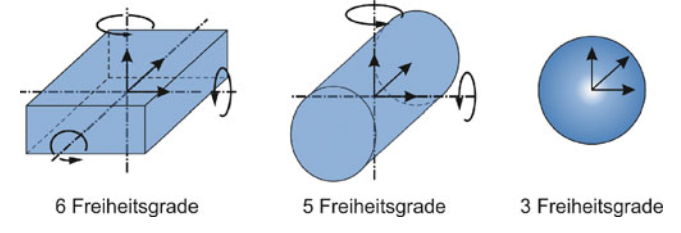
\includegraphics[width=0.8\textwidth]{graphics/intro/intro_freiheitsgrade}
    \caption[Freiheitsgrade diverser Starrkörper]{Freiheitsgrade diverser Starrkörper, \\Quelle: Eigene Abbildung (nach Keferstein Fertigungsmesstechnik)}
    \label{fig:intro_freiheitsgrade}
\end{figure}

Die Qualität eines Robotersystems wird insbesondere daran gemessenen, wie gut eine gewünschte Pose abgebildet werden kann, das heißt wie sehr die sechs Parameter der Ist-Pose mit jenen der Soll-Pose übereinstimmen. Wichtige Kenngrößen für die Bewertung dieser Fähigkeit sind Genauigkeit, Präzision und Auflösung. Abbildung \ref{fig:intro_genauigkeit} stellt den Zusammenhang dieser Größen am bekannten Zielscheibenmodell dar.

\begin{figure}[H]
    \centering
    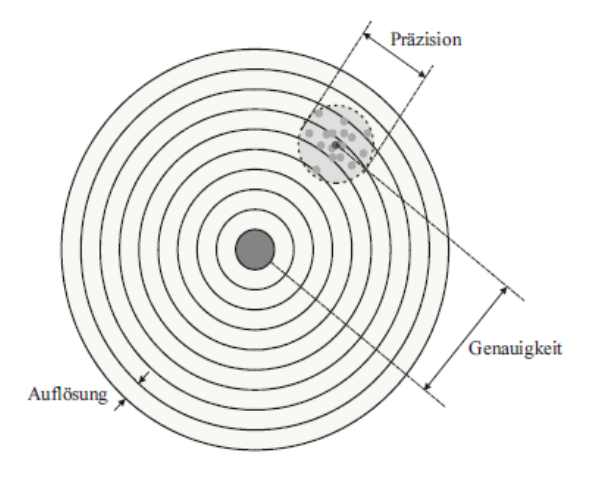
\includegraphics[width=0.7\textwidth]{graphics/intro/intro_genauigkeit}
    \caption[Folie]{Genauigkeit gegenüber Präzision und Auflösung, Quelle: Eigene Abbildung (nach Testo Messunsicherheitsfibel)}
    \label{fig:intro_genauigkeit}
\end{figure}

Die Auflösung, dargestellt als Abstand zwischen den konzentrischen Kreisen der Zielscheibe, entspricht dem kleinsten vom Regler des Robotersystems erfassbaren Bewegungsinkrements, also dessen kleinster Schrittweite. Enstsprechend werden hohe Auflösungen wiederum durch Verwendung  hochauflösender Stell- und Messglieder erreicht. Unter Präzision (auch Wiederholgenauigkeit) wird die Güte der Reproduzierbarkeit bei wiederholtem Einnehmen derselben Pose verstanden. Sie ist ein Maß für die Streuung der Einzelpose und damit eine statistische Abweichung. Die Präzision eines Robotersystems wird hauptsächlich durch dessen Auflösung bestimmt. Die Genauigkeit (auch Absolutgenauigkeit) eines Robotersystems beschreibt den Grad an Übereinstimmung zwischen tatsächlicher Pose und richtiger Pose des End-Effektors. Ein Robotersystem ist genau wenn es sowohl eine hohe Präzision als auch eine hohe Richtigkeit hat. Entsprechend ist hohe Präzision notwendig aber noch nicht hinreichend für hohe Genauigkeit. Ein Mangel an Richtigkeit, sofern bekannt und von systematischer Natur kann durch Kalibrierung verringert werden. (siehe Abbildung \ref{fig:intro_verbesserung_genauigkeit})

\begin{figure}[H]
    \centering
    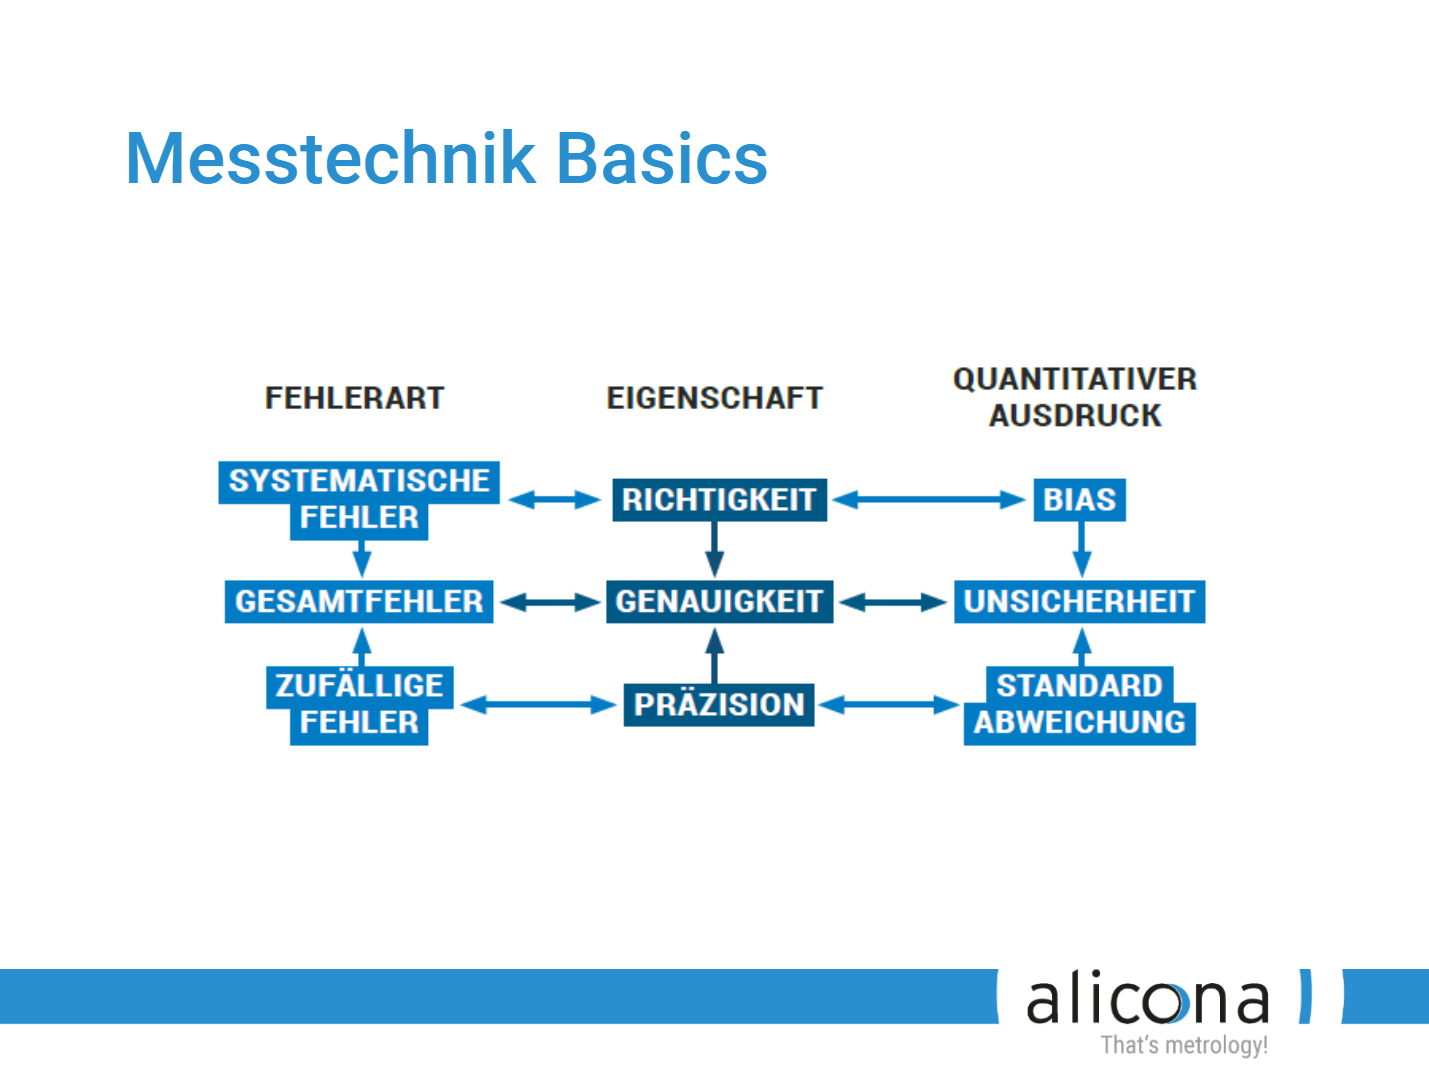
\includegraphics[width=1\textwidth,trim={5cm 8cm 5cm 9cm},clip]{graphics/intro/intro_alicona_basics}
    \caption[Folie]{Genauigkeit, Präzision, Richtigkeit, Quelle: Eigene Abbildung (nach Alicona Präsentation "optische oberflöchen - messtechnik")}
    \label{fig:intro_verbesserung_genauigkeit}
\end{figure}

\begin{figure}[H]
    \centering
    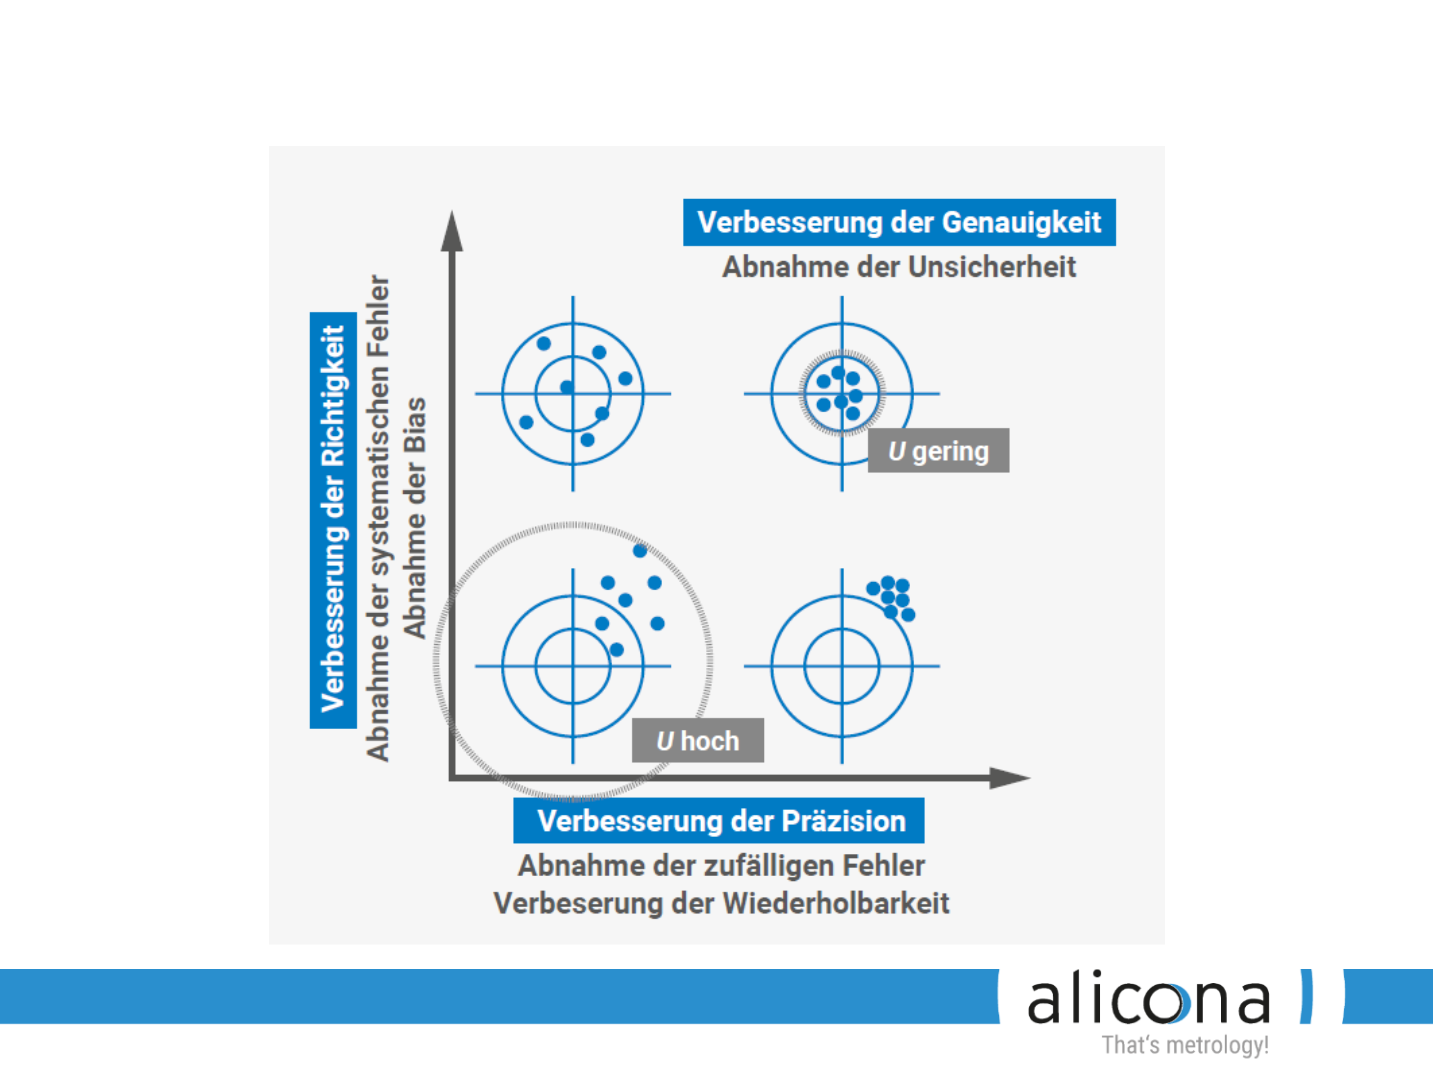
\includegraphics[width=0.7\textwidth,trim={8cm 4cm 8cm 4cm},clip]{graphics/intro/intro_verbesserung_der_genauigkeit}
    \caption[Folie]{Verbesserung der Genauigkeit, Quelle: Eigene Abbildung (nach Alicona Präsentation "optische oberflöchen - messtechnik")}
    \label{fig:intro_verbesserung_genauigkeit}
\end{figure}

Typischerweise haben Robotersysteme vergleichsweise hohe Präzision, aber nur geringe Genauigkeit. Dies ist hauptsächlich darauf zurückzuführen, dass bei den meisten Kinematiken die Pose des End-Effektors nicht oder nur unter großem Aufwand erfasst werden kann. Entsprechend werden Positionsabweichungen nicht am End-Effektor sondern fernab an den angetriebenen Gelenken durch eindimensionale Längen- oder Winkelmessgeräte erfasst. Die einschlägige Literatur unterscheidet zwischen Regelstrategien auf Basis von \emph{joint-space} und \emph{task-space}, also ob die entsprechenden Positionsabweichungen an den Gelenken oder am End-Effektor bestimmt werden. Besonders bei Kinematiken mit sechs Freiheitsgraden gilt die Istwert-Erfassung auf Basis von \emph{task-space} als äußerst schwierig.\footcite[Vgl.][671]{Ting2013} 

Die \emph{joint-space}-Strategie hat den entscheidenden Nachteil, dass viele auf die Genauigkeit des Robotersystems Einfluss nehmende Faktoren unzureichend bis gar nicht berücksichtigt werden können. Zu diesen Faktoren zählen Fertigungsgenauigkeiten der mechanischen Struktur, Nachgiebigkeiten auf Grund von Krafteinwirkungen, thermisch bedingte Verformungen sowie Spiel, Reibungseffekte und andere. Entsprechend werden Robotersysteme bewusst hinsichtlich hoher Struktursteifigkeit und Spielfreiheit konzipiert um diese nicht erfassbaren Einflüsse möglichst konstruktiv zu minimieren. Kinematiken mit mangelhafter Struktursteifigkeit können ausschließlich durch direkte Messung im Sinne der \emph{task-space}-Strategie hohe Genauigkeiten erzielen.\footcite[Vgl.][20-21]{Spong2004}

\begin{em}
The accuracy of a manipulator is a measure of how close the manipulator can come to
a given point within its workspace. Repeatability is a measure of how close a manipulator can return to a previously taught point. Most present day manipulators are highly
repeatable but not very accurate. The primary method of sensing positioning errors in
most cases is with position encoders located at the joints, either on the shaft of the motor
that actuates the joint or on the joint itself. There is typically no direct measurement of
the end-effector position and orientation. One must rely on the assumed geometry of the
manipulator and its rigidity to infer (i.e., to calculate) the end-effector position from the
measured joint angles. Accuracy is affected therefore by computational errors, machining
accuracy in the construction of the manipulator, flexibility effects such as the bending of
the links under gravitational and other loads, gear backlash, and a host of other static and
dynamic effects. It is primarily for this reason that robots are designed with extremely
high rigidity. Without high rigidity, accuracy can only be improved by some sort of direct sensing of the end-effector position, such as with vision.Once a point is taught to the manipulator, however, say with a teach pendant, the above
effects are taken into account and the proper encoder values necessary to return to the given
point are stored by the controlling computer. Repeatability therefore is affected primarily by
the controller resolution. Controller resolution means the smallest increment of motion
that the controller can sense. The resolution is computed as the total distance traveled by
the tip divided by 2n, where n is the number of bits of encoder accuracy. In this context,
linear axes, that is, prismatic joints, typically have higher resolution than revolute joints,
since the straight line distance traversed by the tip of a linear axis between two points is
less than the corresponding arclength traced by the tip of a rotational link.
In addition, as we will see in later chapters, rotational axes usually result in a large
amount of kinematic and dynamic coupling among the links with a resultant accumulation
of errors and a more difficult control problem. \footcite[Vgl.][20-21]{Spong2004}
\end{em}

\begin{em}
Let us examine more closely the current technology behind robot mechanisms. The links are moved by actuators, which typically are electrically driven
(e.g., by DC or AC motors, stepper motors, or shape memory alloys) but can
also be driven by pneumatic or hydraulic cylinders. In the case of rotating electric motors, these would ideally be lightweight, operate at relatively low rotational speeds (e.g., in the range of hundreds of RPM), and be able to generate
large forces and torques. Since most currently available motors operate at low
torques and at up to thousands of RPM, speed reduction and torque amplification are required. Examples of such transmissions or transformers include
gears, cable drives, belts and pulleys, and chains and sprockets. These speedreduction devices should have zero or low slippage and backlash (defined as
the amount of rotation available at the output of the speed-reduction device
without motion at the input). Brakes may also be attached to stop the robot
quickly or to maintain a stationary posture.
Robots are also equipped with sensors to measure the motion at the joints.
For both revolute and prismatic joints, encoders, potentiometers, or resolvers
measure the displacement and sometimes tachometers are used to measure velocity. Forces and torques at the joints or at the end-effector of the robot can be
measured using various types of force torque sensors. \footcite[Vgl.][1-2]{Lynch2017} 
\end{em}

\section{Parallelkinematische Maschinen und Hexapoden}

\begin{figure}[H]
    \centering
    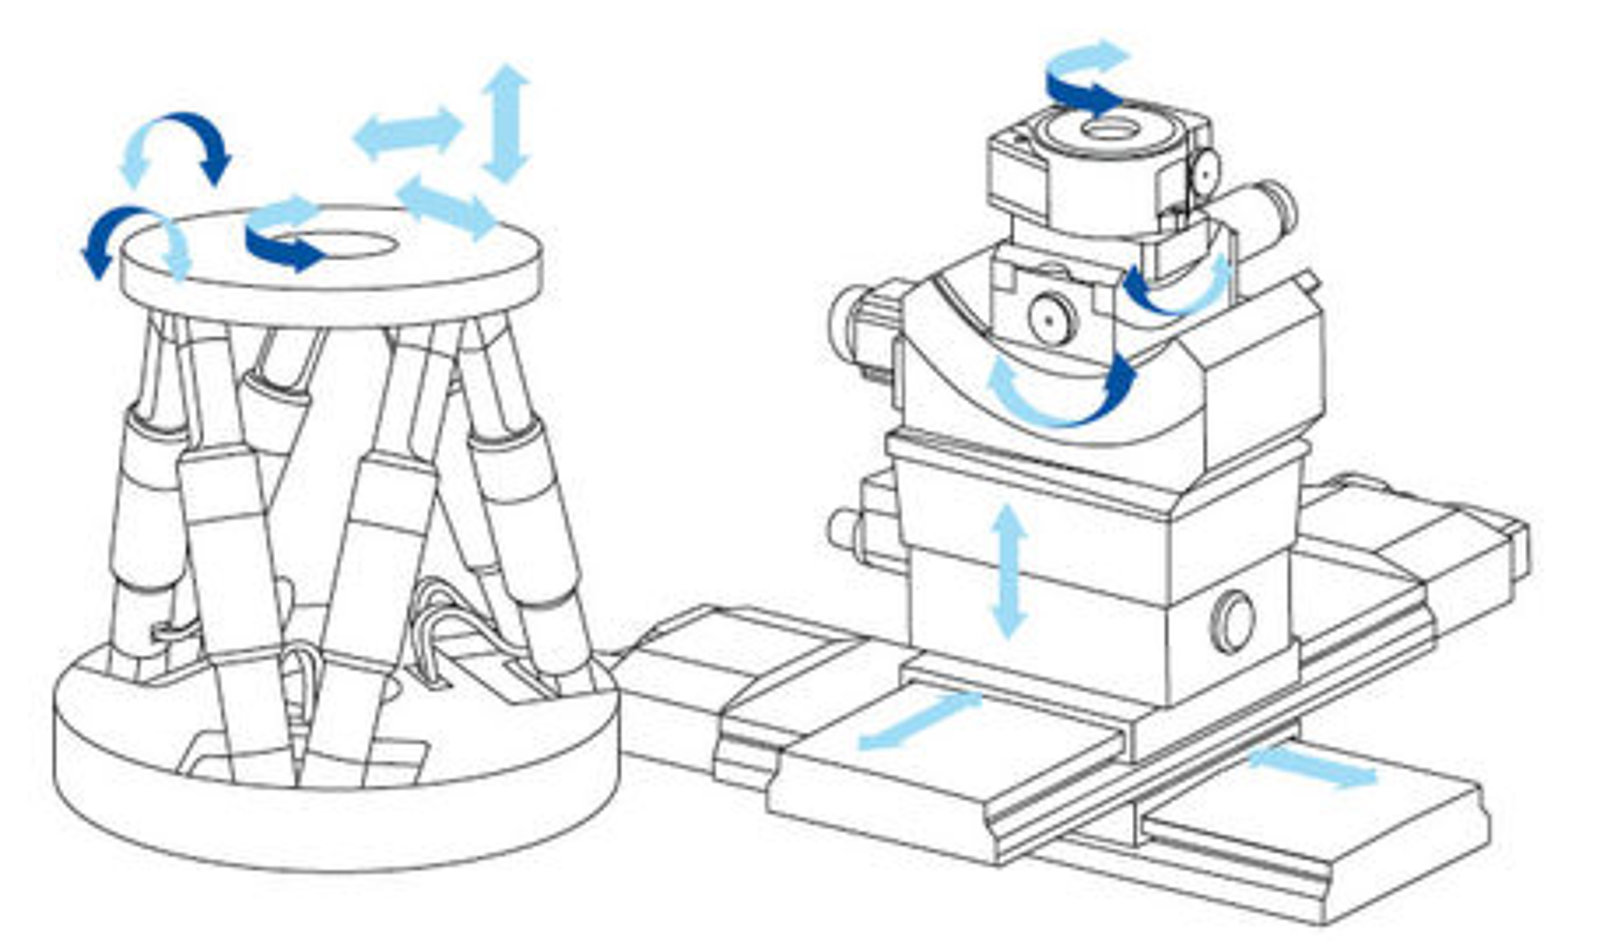
\includegraphics[width=0.7\textwidth]{graphics/intro/intro_pkm_advantages.jpg}
    \caption[Folie]{Parallel- vs Seriellkinematiken, \\Quelle: Physik Instrumente)}
    \label{fig:intro_verbesserung_genauigkeit}
\end{figure}

Hexapod-Kinematiken sind Mechanismen mit geschlossenen kinematischen Ketten welche in verschiedensten technischen Anwendungen zur Manipulation von Objekten eingesetzt werden. Diese Robotersyteme gehören zur Gruppe der Parallelkinematischen Maschinen (PKM) und zeichnen sich im Besonderen durch gute Werte hinsichtlich Traglastverhalten, Struktursteifigkeit und Genauigkeit bzw. Präzision aus. Dementsprechend haben sich Hexapod-Kinematiken in Bereichen durchgesetzt in denen eine oder mehrere dieser Eigenschaften gefordert sind, wie beispielsweise für Flugsimulatoren und Weltraumteleskope aber auch zur Feinpositionierung in der Nanotechnologie und im Prüf- und Messwesen. 

Hexapod-Kinematiken aus den zuletzt genannten Bereichen sind Präzisionsmaschinen und sind Gegenstand der Untersuchungen dieser Arbeit.

Während Hexapoden für die Nanotechnik Genauigkeiten bis in den einstelligen Nanometer-Bereich aufweisen, unterliegen sie jenen für das Prüf- und Messfeld in der Größe ihrer Verstellwege, also ihres Arbeitsraums. Bedingt ist diese Kluft durch grundsätzlich gänzlich unterschiedlich Ausführungen der Gelenke und Linearantriebe. So sind nanometergenaue Kinematiken zwangsläufig mit Festkörpergelenken und Piezoverstellern ausgeführt, wo im Gegensatz jene der anderen Gruppe auf wälz- oder gleitgeführte Gelenke und elektromotorische Antriebe mit Spindeln setzen. Durch die immer höheren Anforderungen noch genauer Messen zu können besteht der Bedarf an Positioniervorrichtungen die bei gleichzeitig großen Arbeitsräumen noch im Sub-Mikrometer-Bereich positionieren können. Diese Hybrid-Maschinen sollen in weiterer Folge als nanoskalige Hexapod-Kinematiken bezeichnet werden und sind Gegenstand der Untersuchungen dieser Arbeit.


%%%%%%%%%%
\begin{em}
Mechanical systems that allow a rigid body (here called an end-effector)
to move with respect to a fixed base, play a very important role in numerous applications. A rigid body in space can move in various ways, in
translation or rotary motion. These are called its degrees of freedom. The
total number of degrees of freedom of a rigid body in space cannot exceed 6 (for example three translatory motions along mutually orthogonal
axes, and three rotary motions around these axis). The position and the
orientation of the end-effector (here called its pose) can be described by
its generalized coordinates; these are usually the coordinates of a specific
point of the end-effector and the angles that define its orientation, but may
be any other set of parameters that allows one to define uniquely the pose
of the end-effector. As soon as it is possible to control several degrees of
freedom of the end-effector via a mechanical system, this system can be
called a robot.\footcite[Vgl.][1]{Merlet2006}
\end{em}

\begin{em}
The low transportable load and poor accuracy are both inherent in the
mechanical architecture of existing manipulators, and in particular of the
serial disposition of the links. Each of them has to support the weight of the
segments following it in addition to the load: they are therefore all subject
to large flexure torques, which means they must be stiffened, and thus
become heavier. Positioning accuracy obviously depends on the flexural
deformations that are not measured by the robot internal sensors. Moreover
the links magnify errors: a small measurement error in the internal sensors
of the first one or two links will quickly lead to a large error in the position
of the end-effector. For example, for a one meter long arm made up of just
one revolute joint, a measurement error of 0.06 degrees leads to an error
of 1 mm in the position of the end-effector. The presence of a drive with a
reduction gear also induces a backlash which leads to inaccuracy. The violation of the assumed geometric constraints between the axes of
the links also constitutes an important source of positioning errors. A slight
perpendicularity error between the first two axes of a spherical manipulator
will lead to errors in all vertical motions that, given the amplitude of the
motions, must be taken into account. Note that the successive positions of
the links, together with the necessity of stiffening them, imply that the moving parts of the robot will have a significant mass. As a consequence, during
high velocity motions, the manipulator experiences inertia, centrifugal and
Coriolis forces that make the control of the robot complex.
Serial robots operate under the action of two kind of forces: inertia and
friction. These forces have different scales: inertia forces essentially vary
with the square of the lengths of the links; friction forces are relatively unaffected by such dimensions. This means that one cannot design a micro
serial robot simply by scaling down a larger version; under such scaling,
the inertia forces are reduced while the friction forces remain relatively unchanged. We conclude that serial robots are inappropriate for tasks requiring either the manipulation of heavy loads, or a good positioning accuracy,
or to work at different scales.\footcite[Vgl.][4]{Merlet2006}
\end{em}

\begin{em}
Mechanical systems that allow a rigid body (here called an end-effector)
to move with respect to a fixed base, play a very important role in numerous applications. A rigid body in space can move in various ways, in
translation or rotary motion. These are called its degrees of freedom. The
total number of degrees of freedom of a rigid body in space cannot exceed 6 (for example three translatory motions along mutually orthogonal
axes, and three rotary motions around these axis). The position and the
orientation of the end-effector (here called its pose) can be described by
its generalized coordinates; these are usually the coordinates of a specific
point of the end-effector and the angles that define its orientation, but may
be any other set of parameters that allows one to define uniquely the pose
of the end-effector. As soon as it is possible to control several degrees of
freedom of the end-effector via a mechanical system, this system can be
called a robot.\footcite[Vgl.][1]{Merlet2006}
\end{em}

\begin{em}
Currently, most existing manipulators present a decidedly anthropomorphic
character, usually strongly resembling a human arm. They are constituted
of a succession of rigid bodies, each of them being linked to its predecessor
and its successor by a one-degree-of-freedom joint, for example allowing
the rotation of a rigid body around an axis , or the translatory motion of a
rigid body. This architecture will be called a serial robot with analogy to
electrical systems. An example of a serial mechanism is the spherical robot,
where a succession of segments goes from the base to the end-effector, each
segment being linked to its successor by a revolute joint. If each of the n
joints is actuated, it will usually be possible to control n degrees of freedom of the end-effector.\footcite[Vgl.][1-2]{Merlet2006}
\end{em}

Parallelkinematiken haben eigentlich keine Baugruppen, die im geometrischen Sinne parallel zueinander sind. Woher der Begriff kommt, verdeutlicht Abb. 1.1. Bei einer konventionellen seriellen Struktur sind alle Bewegungsachsen nacheinander angeordnet. Die erste Schwenkachse trägt z. B. die zweite Schwenkachse; diese wiederum trägt die translatorische Achse. Jede weitere Achse ergänzt den Mechanismus um einen weiteren Freiheitsgrad. Dabei handelt es sich um eine offene kinematische Kette; jeder Antrieb wird mit den Massen der nachfolgenden Glieder und Antriebe
belastet. Die steigenden Anforderungen an die dynamischen Eigenschaften von Maschinen führen daher in ein Dilemma: Werden leistungsfähigere Antriebe in Kombination mit zusätzlichen Versteifungen verwendet, erhö-
hen sich die zu bewegenden Massen. Dies erfordert wiederum eine Steigerung der Antriebsleistung, die mit weiterer Massevergrößerung verbunden ist usw. werden. Es entstehen so genannte geschlossene kinematische Ketten, wodurch u. a. eine Parallelschaltung der Steifigkeiten der einzelnen Ketten erreicht wird. Bei rein paralleler Bauweise enthält jede Kette genau einen Antrieb, so dass die Anzahl der Gelenkketten mit dem Freiheitsgrad der Struktur übereinstimmt. Mechanismen, die innerhalb einer Gelenkkette über mehrere Antriebe verfügen, bezeichnet man als hybride Parallelkinematiken. Im Gegensatz dazu greifen bei einer Parallelkinematik alle Bewegungsachsen direkt oder dicht an der zu bewegenden Arbeitsplattform an. Um eine gewünschte Bewegung auszuführen, müssen alle Antriebe bewegt werden. Es entstehen so genannte geschlossene kinematische Ketten, wodurch u. a. eine Parallelschaltung der Steifigkeiten der einzelnen Ketten erreicht wird. Bei rein paralleler Bauweise enthält jede Kette genau einen Antrieb, so dass die Anzahl der Gelenkketten mit dem Freiheitsgrad der Struktur übereinstimmt. Mechanismen, die innerhalb einer Gelenkkette über mehrere Antriebe verfügen, bezeichnet man als hybride Parallelkinematiken. 
\footcite[Vgl.][1-2]{Neugebauer2006}

Parallelkinematiken weisen im Vergleich zu seriellen Kinematiken eine
ganze Reihe von Vorteilen auf. Besonders hervorzuheben sind die geringen zu bewegenden Massen sowie die günstigen dynamischen Eigenschaften. Bei entsprechender Wahl der Gelenke werden die Glieder überwiegend auf Druck oder Zug beansprucht. Im Vergleich zu Industrierobotern ist besonders die hohe Wiederholgenauigkeit hervorzuheben. Natürlich gibt es auch Nachteile, so z. B. der im Verhältnis zum Bauraum relativ kleine Arbeitsraum, die teilweise geringen Schwenkwinkel und die durch Koordinatentransformation aufwändige Steuerung. Ein weiterer Nachteil gegenüber Präzisions-Werkzeugmaschinen sind die noch zu geringen absoluten Positioniergenauigkeiten. Auch Entwicklung und Optimierung angepasster Maschinenelemente wie Kardan- und Kugelgelenke bieten noch Handlungsbedarf. \footcite[Vgl.][2]{Neugebauer2006}

Einige Jahre später wurde ein parallelkinematischer Mechanismus entwickelt, der Berühmtheit erlangte und tausendfach nachgebaut wurde: die auf dem (damals schon längst bekannten) Hexapod\-Prinzip basierende Reifenprüfeinrichtung des Engländers Eric Gough, der für die DUNLOP RUBBER CO. in Birmingham arbeitete. Ziel der Entwicklung war, die Eigenschaften von Flugzeugreifen unter verschiedensten Belastungsbedingungen testen zu können, Abb. 1.4. \footcite[Vgl.][4]{Neugebauer2006}

\begin{em}
A parallel manipulator is one in which the links form a closed chain. More specifically, a
parallel manipulator has two or more independent kinematic chains connecting the base to
the end-effector. Figure 1.19 shows the ABB IRB 940 Tricept robot, which has a parallel
configuration. The closed chain kinematics of parallel robots can result in greater structural
rigidity, and hence greater accuracy, than open chain robots.\footcite[Vgl.][18]{Spong2004}
\end{em}

\begin{em}
Parallel robots, also sometimes called hexapods or Parallel Kinematic Machines (PKM), are closed-loop mechanisms presenting very good performances in terms of accuracy, rigidity and ability to manipulate large loads.
They are been used in a large number of applications ranging from astronomy to flight simulators, and are becoming increasingly popular in the
machine-tool industry.\footcite[Vgl.][XV]{Merlet2006}
\end{em}
%%%%%%%%%%

\section{Problemstellung}

\section{Ziel der Arbeit}

\section{Aufbau der Arbeit}

\section{Paper-Zitate}

\subsection{Ting: Measurement and calibration for Stewart micromanipulation system}
Micro-positioning technique becomes very important for
precision engineering in various application areas such as semiconductor, biomedical science, optics and microscopy. Several
popular micro-positioning platforms, for example, the scanners of STM, AFM, 6-dof hexagonal structures have been used
widely. Since the demand of high precision, the unavoidable
errors come from the mechanism manufacture and from the
assembly are critical factors.\footcite[Vgl.][226]{Ting2007}

Piezoelectric actuator is of good response, high stiffness,
nanometer output, less EMI effect, etc. It is quite suitably used
for micro-positioning platform. However, the hysteresis effect,
which reduces the response, is an obvious and serious problem in
high precision engineering.\footcite[Vgl.][226]{Ting2007}

Via the inverse kinematics between the
joint and the end-effector and the interpolation method on the
assumption of small variation, an error compensation model is
developed to calibrate the platform output with good accuracy
of about 1 m in position and 10 degree in orientation.\footcite[Vgl.][266]{Ting2007}

A 6-dof Stewart type micro-positioning platform driven by
stack type piezoelectric actuators, and employed universal joints
is shown in Fig. 1. Each actuator canreach themaximum longitudinal displacement of 160 m with the input voltage up to 150 V. \footcite[Vgl.][226]{Ting2007}

According to the inverse hysteresis
model in Section 4, the error is in the range of 0.1 m. However,
in fact, the measurement on the end-effector shows large error
existing, which is mainly caused by manufacture and assembly
errors. Thus, error compensation method is applied to deal with
the problem.\footcite[Vgl.][232]{Ting2007}

\subsection{Ting: Composite controller design for a 6DOF Stewart nanoscale platform}
In many applications of semiconductor, bioengineering, optics
and so on, demand of high precision reaches nanoscale. A few of
nanoscale platforms have been designed for those applications
[1–5]. In general, piezoelectric actuator is used for the driving
resource because of its good characteristics of precise movement
and miniature resolution.Unavoidable errors creep in during
mechanism manufacture and from assembly and nonlinearity of
the piezoelectric actuator, which makes difficulties for precision
control.\footcite[Vgl.][671]{Ting2013}

An attempt of
improving the target of nanoscale, flexural joints are used to
connect the legs with the upper (movable) and lower (fixed)
platforms to form a new 6DOF Stewart-type platform as presented in Fig. 1. \footcite[Vgl.][671]{Ting2013}

For serial or parallel robots, most of
the robot control methods are designed on the basis of joint space.
Although task-space control can control on the end-effector (the target), the difficulty on task-space measurement on-line makes
it impractical. Using forward kinematics to compute the pose of
the end-effector by means of the measured joint variables is likely
workable in parallel robot. However, the solution is not unique and
determination of numerous possible solutions is quite complex
and unreliable [11]. Measure of the pose of the end-effector
is demanding. In this study, a sensor holder is built to install
sensors located below the upper platform. Associated with the
developed measurement method, the pose of the end-effector can
be measured directly, thus the on-line task-space control purpose
is achieved. Structure compliance of the platform and external
load variation in insertion task application is concerned. Lyapunov
function is used to determine a robust control rule with bounded
model error along with a PID control. By use of relay feedback test
method and genetic algorithm, optimal gains of PID are searched. \footcite[Vgl.][671]{Ting2013}

A new measurement method is developed to directly measure
the end-effector of the 6DOF nanoscale platform. As illustrated in
Fig. 1, a sensor holder is designed and mounted on the base in the
hollow space of the platform [12]. Entire configuration of the sensor
employment is illustrated in Fig. 5. A nanoscale sensor (Lion Precision, Probe Model: C6-D, Driver Model: DMT22) is used, which
provides resolution: 2.2 nm for large stroke in a range of 50 m and resolution: 0.4 nm for fine stroke in a range of 10 m. As illustrated in Fig. 5, in the XY plane, sensor #1 is employed along the y
axis and sensor #2 is employed along the x axis and sensor #3 is
employed with a distance D away from sensor #2 and in the direction parallel to the y axis. Similarly, in the YZ and ZX plane, sensor
#4 is located at the center; sensors #5 and #6 are employed with a
distance D away from the center and along the y and x axes respectively. Thus, sensors #2 and #3 are in charge of measurement in
the X direction, and sensor #1 for the Y direction, and sensor #4,
#5, #6 for the Z direction. Also, a light cuboid is mounted on the
upper platform with the assigned measure points (S1, S2, S3, S4, S5,
S6) shown in Fig. 6 for the corresponding sensors (#1, #2, #3, #4,
#5, #6). By use of the measured data, the parameters ( dx, dy, dz, drx, dry, drzz) of the moving platform are obtained and listed in
Table 2. The computation procedures are described as below. \footcite[Vgl.][673-674]{Ting2013}

Note that there are two types of measurement error need concern. One is the surface of the measurement sensors, for example
sensors #2 and #3 at measure points (S2, S3), should be in parallel with the surface of the movable platform; the other one is the
computation error of rotating angle due to multiple rotations. The
former one can be calibrated by using the pair of sensors to measure the surface of the movable platform. That is, in case the surfaces
are not parallel, the measured distance to the movable platform is
different. The difference can be found in advance for error compensation. The latter one is defined by geometric relationship and
proved to be very small and negligible. However, the error can be
computed during manipulation for error compensation. \footcite[Vgl.][674]{Ting2013}

It is seen that in free-space manipulation, the average error norm of translation and orientation in the manipulation
period for feedforward, feedback, and composite is (284 nm,
96 nrad), (56 nm, 29 nrad), (17 nm, 5 nrad) respectively, and the maximum error norm is (540 nm, 195 nrad), (126 nm, 29 nrad),
(46 nm, 20 nrad) respectively. The composite controller is superior
to the others.\footcite[Vgl.][680-683]{Ting2013}

It is obviously seen that the composite controller
outperforms the other two methods. Especially, through the measured pose of the end-effector, the contact force is then computed
(18) with the already known stiffness Kr = diag{0.114, 0.104, 0.086,
138.839, 185.135, 166.67}. As seen, the tracking error is drastically reduced while the equivalent contact force is included in
(19). \footcite[Vgl.][683]{Ting2013}

The results show that all
methods reach nanoscale class of precision. Without using expensive sensors, the feedforward controller alone is able to overcome
the hysteresis effect and nearly achieve the nanoscale target especially with no external load. In case the precision scale is acceptable,
it is a cost-effective design for the application purposes of free space
motion. As expected, the proposed composite controller performs
much better than the feedforward and feedback controller alone.
Further experiments for more complex application encountered
with external force or torque from various directions will be tackled
in the near future.\footcite[Vgl.][683]{Ting2013}

\subsection{Shi: Kinematic modeling and calibration of a flexure based hexapod nanopositioner}
Flexure or compliant mechanisms [1] composed of flexure
hinges and leaf springs have the advantage of no backlash and
ultrahigh precision. They have been widely used in precision
nanopositioners or naomanipulators which play an important
role in emerging nanotechnology [2]. Compliant parallel platform
mechanisms combine the advantages of flexure mechanisms and
parallel platforms, and have received particular attention from nanotechnologists [3–7]. However, modeling and controller design has
been a challenging task due to their inherent structural complexity and difficulties in measuring the six-degree-of-freedom (6DOF)
positioning accuracy.
Kinematic calibration is the mapping of the output movement
relative to the input to the actuators by means of physical experiments. It is one of the key steps in the development of a controller.\footcite[Vgl.][117]{Shi2013} 

In conclusion, we have presented a two-phase platform calibration method for a hexapod nanopositioner. First, a kinematic
model is derived for the nanopositioner platform. Next, a new
calibration set for the platform is determined using an interferometer and an autocollimator to measure the displacements
in six degrees of freedom. Kinematic-model-based calibration
is used to get more accurate results. The results show that
the maximum of rotational error is 0.0024◦ and the maximum
of translational error is 3.34 m. In future work, a controller
would be developed based on the calibrated Jacobian matrix.
Furthermore, this calibration method can be applied to a smallscale hexapod platform realized using microelectromechanical
systems.\footcite[Vgl.][124]{Shi2013}



%-----------------------------------------------------------------------------------------------%
%\chapter{Dummy}
%\section{Figure}
\blindtext[1]
\begin{figure}[H]
    \centering
    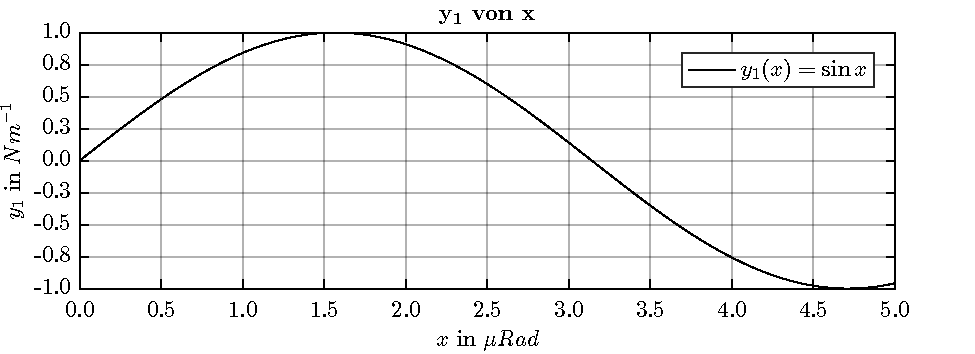
\includegraphics{graphics/dummy/fig_y1.pdf}
    \caption{Caption}
    \label{fig:my_label}
\end{figure}
%\blindtext[1]
\begin{figure}[H]
    \centering
    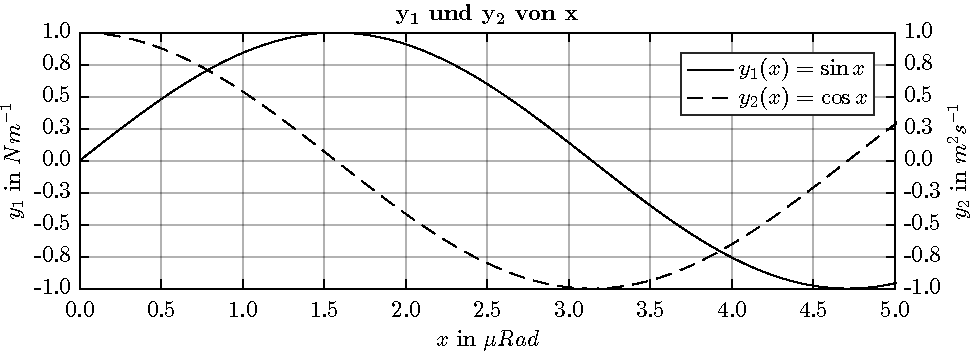
\includegraphics{graphics/dummy/fig_y2.pdf}
    \caption{Caption}
    \label{fig:my_label}
\end{figure}
\blindtext[1]
\begin{figure}[H]
    \centering
    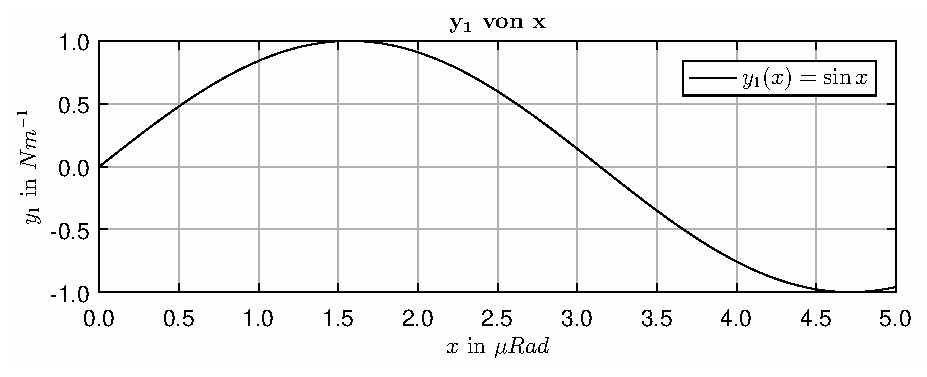
\includegraphics{graphics/dummy/fig_y1.eps}
    \caption{Caption}
    \label{fig:my_label}
\end{figure}
\section{Table}
\input{chapters/dummy/table.tex}
%-----------------------------------------------------------------------------------------------%
\chapter{Grundlagen}
%---------------------------------------------------------------------------------------------%
\section{Aufbau von Hexapoden}
\label{sec:aufbau}
\section{Parallelkinematische Maschinen Neugebauer}

\begin{itemize}
    \item kinematische Struktur
    \item Systematisierung anhand der Ordnungskriterien „Freiheitsgrad“, „Anzahl der Führungsketten“ und „Anzahl der Antriebe“ verwendet
\end{itemize}

\subsection{Struktursystematik}
Parallelkinematische Mechanismen sind – aus getriebetechnischer Sicht betrachtet – ungleichmäßig übersetzende Mechanismen. Hinsichtlich ihrer Funktion kann man zwischen Übertragungsgetrieben und Führungsgetrieben unterscheiden. Erstere dienen der Übertragung mechanischer Leistung, bei Letzteren wird ein Getriebeglied so geführt, dass es bestimmte Lagen einnimmt, bzw. dass seine Punkte bestimmte Bahnen, sog. Führungsbahnen, beschreiben [145, 146]. Eine aus energetischer Sicht untergeordnete Rolle spielt bei Führungsgetrieben deren Übertragungsfunktion. Mechanismen mit parallelen Strukturen werden den Führungsgetrieben zugeordnet. Da Getriebe nach ihren charakteristischen Bestandteilen eingeteilt werden können, gehören die hier interessierenden Mechanismen zu den Koppelgetrieben. Die eben betrachteten Kriterien geben den parallelkinematischen Mechanismen einen eindeutigen Platz innerhalb der Ordnung aller Getriebe. Parallelkinematiken sind Führungsgetriebe, bei denen die Arbeitsplattform über mindestens zwei angetriebene Führungsketten mit dem Gestell verbunden ist. \footcite[Vgl.][14]{Neugebauer2006}

\subsection{Grundstrukturen}

\begin{figure}[H]
    \centering
    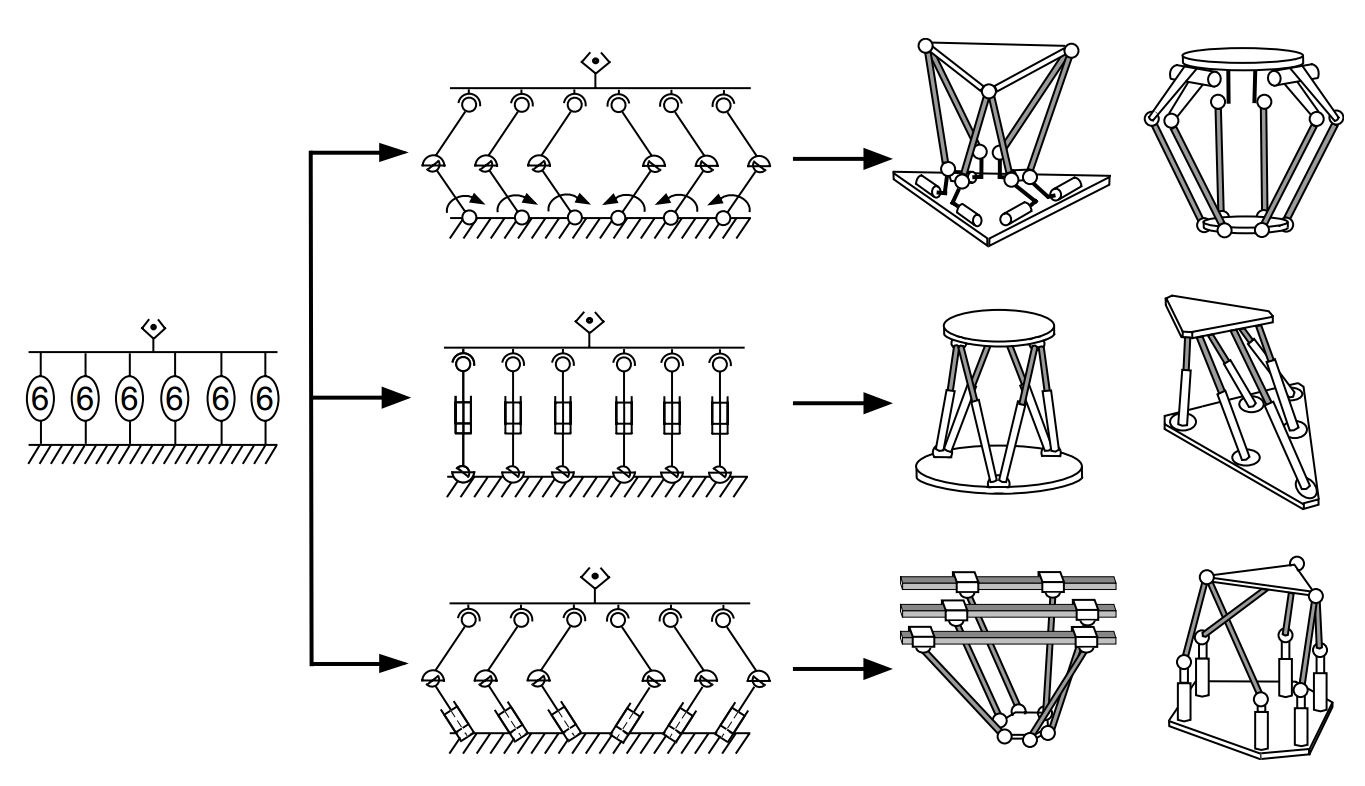
\includegraphics[width=\textwidth]{basics/aufbau/strukturentwicklung}
    \caption[Entwicklung einer Parallelkinematik]{Entwicklung einer Parallelkinematik: vom kinematischen Schema über das kinematische Prinzip zur kinematischen Struktur; Quelle: Neugebauer (2006), Parallelkinematische Maschinen}
    \label{fig:stab1}
\end{figure}

\begin{itemize}
    \item Alle Führungsketten haben genau einen Antrieb mit dem Freiheitsgrad Eins.
    \item Mindestens eine Führungskette hat mehr als einen Antrieb mit dem Freiheitsgrad Eins.
    \item Mindestens eine Führungskette hat keinen Antrieb.
\end{itemize}

Ausgehend von den Gleichungen (2.1) und (2.2) zur Bestimmung des Freiheitsgrades von Mechanismen werden die Mechanismen so abstrahiert, dass nur noch die Anzahl der Führungsketten FK und deren Freiheitsgrad F in die Berechnung eingehen. Der Freiheitsgrad F der Führungsketten wird berechnet aus dem Freiheitsgrad der Führungsketten gemäß Gln. (2.1) und (2.2) plus dem Gelenkfreiheitsgrad des Verbindungsgelenks zwischen Führungskette und Arbeitsplattform. Bei räumlichen Getrieben mit ebenen Teilgetrieben werden letztere gesondert behandelt. Sie werden als Ersatzgelenk mit dem entsprechenden Gelenkfreiheitsgrad in der Freiheitsgradberechnung des räumlichen Getriebes berücksichtigt.

\begin{figure}[H]
    \centering
    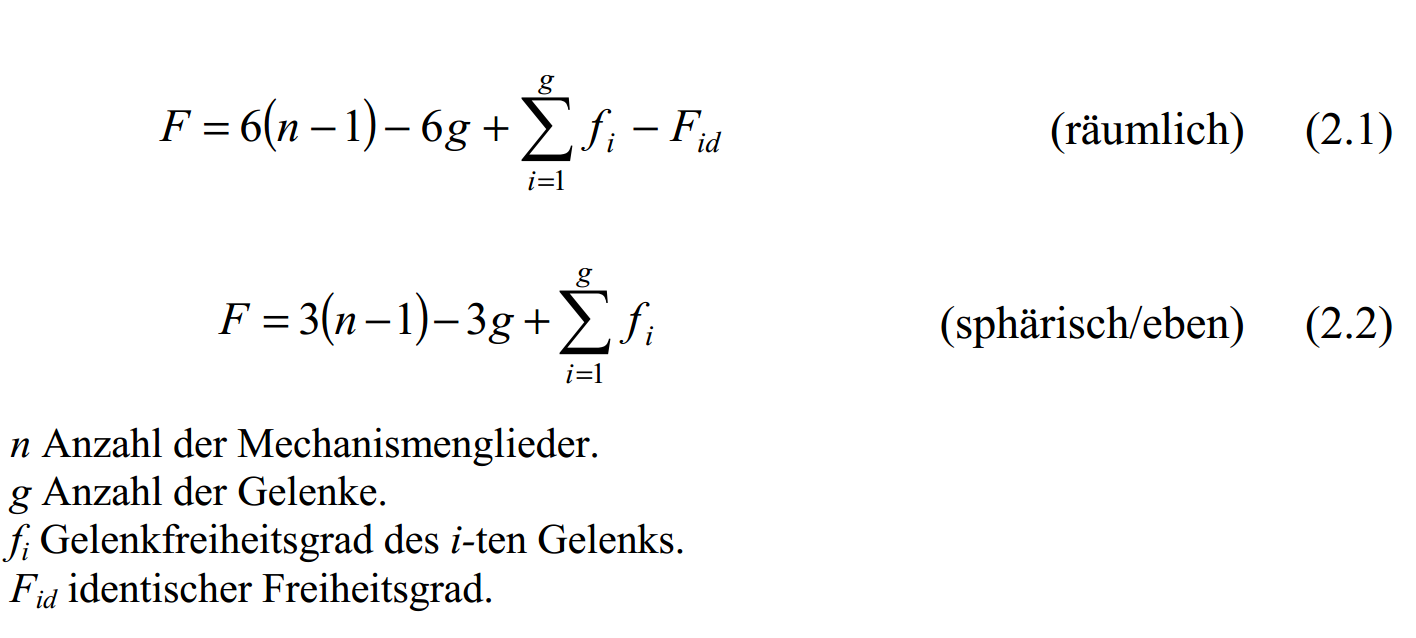
\includegraphics[width=\textwidth]{basics/aufbau/fk_gleichungen}
\end{figure}

Hinzuzufügen ist, dass Führungsketten mit F = 6 mindestens einen Antrieb haben müssen, da sie sonst für den Mechanismus ohne kinematische Bedeutung sind. \footcite[Vgl.][17]{Neugebauer2006}

\begin{figure}[H]
    \centering
    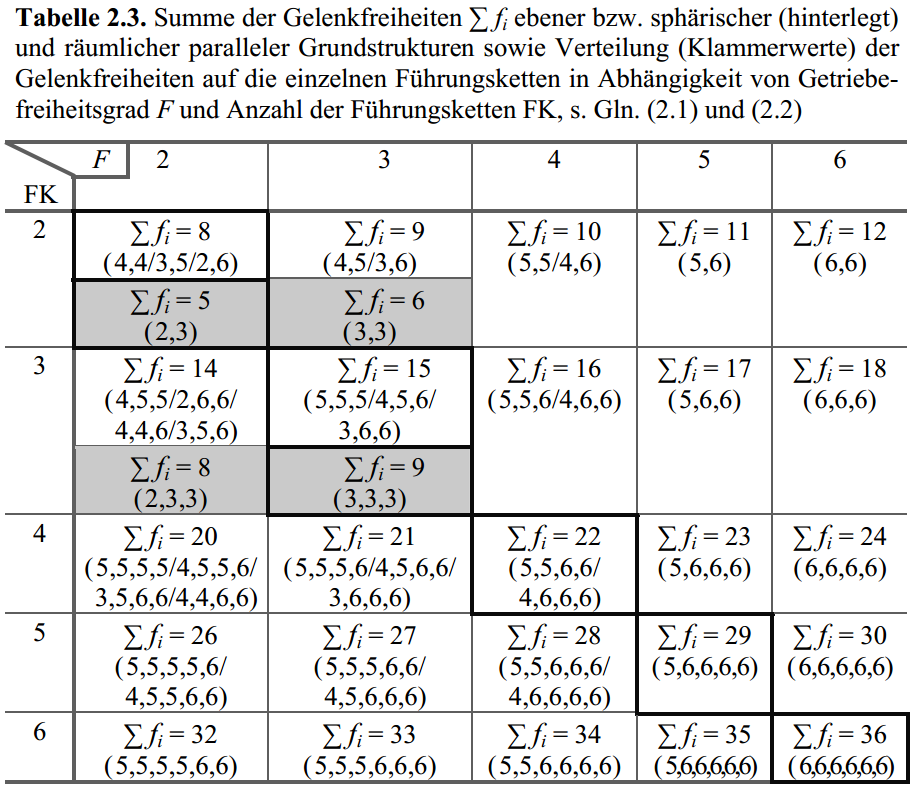
\includegraphics[width=\textwidth]{basics/aufbau/tab_gelenkfreiheiten}
\end{figure}

Parallele Strukturen, in denen jede Führungskette genau einen Antrieb mit dem Freiheitsgrad Eins enthält, werden „vollparallel“ genannt und entsprechen in Tabelle 2.3. allen Schemata entlang der Diagonalen. 

Für die Grundformen der häufig in Parallelkinematiken zur Anwendung kommenden Gelenke werden im Weiteren Bezeichnungen verwendet, die im Wesentlichen auf die z. B. in [30] und [145, 146] vorgestellten zurückgehen:

\begin{itemize}
    \item Drehgelenk (D)
    \item Drehschubgelenk (DS)
    \item Kardangelenk (DD)
    \item Kugelgelenk ($D_3$)
    \item Schubgelenk (S)
\end{itemize}

\begin{figure}[H]
    \centering
    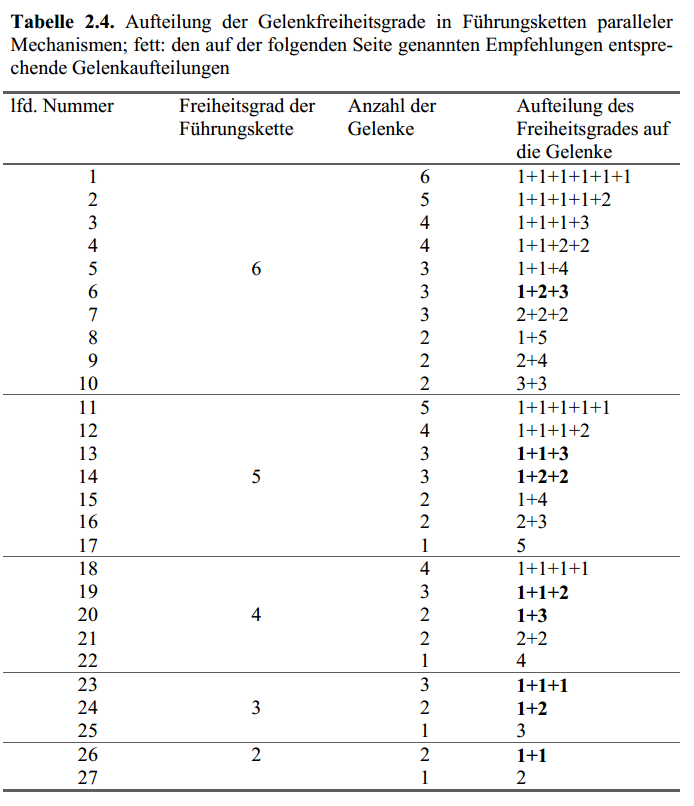
\includegraphics[width=\textwidth]{basics/aufbau/fk_empfehlungen}
\end{figure}

Für die Gestaltung der Führungsketten, d. h. die konkrete Verteilung der Gelenkfreiheiten, sind beliebige Varianten denkbar. Entsprechend Tabelle 2.4. kommen Führungsketten, deren Freiheitsgrad die Bedingung 2 kleiner gleich F kleiner gleich 6 erfüllt, in Betracht. Nachfolgend sind alle Möglichkeiten der Verteilung der Gelenkfreiheiten innerhalb der Führungsketten aufgeführt. Die Reihenfolge kann variiert werden. Der nächste Entwicklungsschritt ist die Zuordnung konkreter Gelenke zu den Gelenkfreiheiten. Dabei ist zu beachten, dass in der bisher vorgestellten Systematik auch solche Grundstrukturen erfasst sind, die einerseits aufgrund einer ungünstigen Gelenkanordnung nicht lauffähig oder andererseits einer zu großen Anzahl von Gelenken wegen praktisch irrelevant sind. Um aber dennoch dem Konstrukteur mit der Entwicklungssystematik ein handhabbares und hilfreiches Werkzeug verfügbar zu machen, müssen diese Grundstrukturen von den praktisch zweckmäßigen und nutzbaren unterschieden werden. Insoweit können folgende einschränkende Forderungen an die konstruktive Ausführung von Führungsketten als Empfehlung geltend gemacht werden:

\begin{itemize}
    \item Aufgrund der Forderung nach linearer Unabhängigkeit der Gelenkachsen dürfen im ebenen Fall maximal zwei und im räumlichen Fall maximal drei Schubgelenke in einer Gelenkkette vorhanden sein.
    \item Die Antriebe müssen gestellnah angeordnet werden, um die zu bewegende Maschinenmasse weitestgehend zu reduzieren. Als Antriebsgelenke sollen Gelenke mit dem Freiheitsgrad Eins verwendet werden.
    \item Die einzelnen Gelenkketten sollten gleichartig aufgebaut sein, um den konstruktiven Aufwand und die Fertigungskosten zu minimieren.
    \item Bei passiven Gelenken sind Drehgelenke gegenüber Schubgelenken aufgrund des geringeren konstruktiven Aufwands zu bevorzugen. Außerdem ist bei passiven Schubgelenken die Klemmgefahr zu beachten. Es sollten nur Gelenke mit einem Gelenkfreiheitsgrad kleiner Vier zum Einsatz kommen.
    \item Eine Führungskette sollte einschließlich der Anschlussgelenke an Plattform und Gestell nur drei Gelenke enthalten, da sonst die Steifigkeit zu gering ist und Fehler durch seriellen Aufbau der Maßketten (Summenfehler) auftreten.
\end{itemize}

Bei mehrfach angetriebenen Führungsketten sind Lösungsmöglichkeiten auf Basis ebener Teilstrukturen zu bevorzugen (Möglichkeit, alle Antriebe gestellnah anzuordnen, bzw. kein serieller Aufbau). Die Antriebe sind so anzuordnen, dass jede Führungskette mindestens eine Freiheit der Plattform bindet. Bezogen auf Führungsketten mit F = 6 bedeutet dies, dass sie mindestens einen Antrieb enthalten müssen. Prinzipiell ist zwischen zwangführenden und nicht-zwangführenden Führungsketten zu unterscheiden. Letztere schränken die Bewegung des Endeffektors nicht ein. Im ebenen Fall sind dafür drei und im räumlichen Fall sechs Gelenkfreiheiten notwendig.

\begin{itemize}
    \item Gelenke $f_i = 2$ Drehschubgelenk; Kardangelenk
    \item Gelenke $f_i = 3$ Kugelgelenk
\end{itemize}
%---------------------------------------------------------------------------------------------%
%---------------------------------------------------------------------------------------------%
\section{Koordinatentransformation}
\label{sec:transformation}
%---------------------------------------------------------------------------------------------%
% Chapter: Koordinatentransformation
%---------------------------------------------------------------------------------------------%
Für die kinematische Modellierung von Hexapoden ist die korrekte Beschreibung ihrer Transformationsgleichungen von elementarer Bedeutung. Folglich sollen in diesem Abschnitt die Grundlagen der Koordinatentransformation in Ebene und Raum wiederholt werden. \\

%Mit den erarbeiteten mathematischen Grundoperationen soll im Anschluss ein Gleichungssystem zur Beschreibung der \glqq 6D-Transformation \grqq einer allgemeinen Hexapod-Kinematik aufgestellt werden.\\
%Die mobile Plattform einer Hexapod-Kinematik lässt sich in sechs Freiheitsgraden bewegen, wobei drei Translationen und drei Rotationen um jede der drei Raumachsen möglich sind. Die mathematische Beschreibung dieser kombinierten Bewegungen erfolgt im Allgemeinen über entsprechende Transformationsmatrizen die eine \glqq 6D-Transformation \grqq in nur einer Matrixoperation ermöglichen. Für die Aufstellung solcher Transformationsgleichungen bedarf es der Festlegung einer Konvention hinsichtlich der Transformationsfolge die sich je nach Anforderung an das kinematische System bzw. die Anwendung unterscheiden kann und damit die spezielle Form der Transformationsmatrix festlegt. Die Transformationsfolge definiert, in welcher Folge die rotatorischen Operationen gereiht sind und ob die Translationen vor oder nach den rotatorischen Transformationen einfließen. Häufige Festlegungen sind die \glqq Euler-Winkel-Konvention \grqq und die \glqq Roll-Nick-Gier-Konvention \grqq. \\

Unter einer Koordinatentransformation wird im Allgemeinen die Übersetzung von einem Koordinatensystem $K = \{O;\bvec{e_{i}}\}$ auf ein gleichartiges System $K^\prime = \{O^\prime;\bvec{e_{i}}^\prime\}$, $i=1,2,\ldots,n$ verstanden. Man unterscheidet zwei grundsätzliche Fälle:

\subsubsection{Fall A - Feststehendes System und bewegtes Objekt} 
Übergang von einer Objektkonfiguration $P$ in eine neue Konfiguration $P^\prime$ wobei das Koordinatensystem $K$ unverändert bleibt. Beispiel: {\color{red}Überwachung vom Flugverkehr mittels Radar, wobei der Kontrolltower das ortsfeste System $K$ stellt und die sich im Luftraum befindlichen Flugzeuge $P_{i}$ relativ zu $K$in eine neue Konfiguration $P_{i}^\prime$ bewegen.}
\subsubsection{Fall B - Bewegtes System und feststehendes Objekt}
Übergang vom System $K$ in ein gleichartiges System $K^\prime$ wobei die Objekte $P_{i}$ nicht transformiert werden. Beispiel: Bearbeitung eines eingespannten, also ortsfesten Werkstücks in einer Werkzeugmaschine. Das Werkzeugkoordinatensystem $K^\prime$ wird hierbei gemäß des CNC-Programms relativ zum Maschinenkoordinatensystem $K$ bewegt. 
\footcite[Vgl.][1-2]{Neugebauer2006}
\footcite[Vgl.][95]{Keferstein2018}
\footcite[Vgl.][8-20]{Wloka1994}
\footcite[Vgl.][38\psqq]{Bartsch2014}
\footcite[Vgl.][33]{Pfeifer2010}
\footcite[Vgl.][12]{Schuth2017}
%---------------------------------------------------------------------------------------------%
% Subsection: Koordinatentransformation in der Ebene
%---------------------------------------------------------------------------------------------%
\newpage
\subsection{Translation in der Ebene}
\label{subsec:translation_2d}
%---------------------------------------------------------------------------------------------%
% Fall A - Verschiebung des Objekts
%---------------------------------------------------------------------------------------------%
\subsubsection{Fall A - Verschiebung des Objekts}
Betrachtet werde ein Punkt $P$ in der $xy$-Ebene, dessen Position durch den Ortsvektor $\bvec{x}$ bestimmt sei, siehe \cref{fig:translation_2d_a}. Mit dem in \cref{eq:translation_2d_1} eingeführten Translationsvektor $\bvec{t}$ erfolgt eine Verschiebung von $P$ nach $P^\prime$. Der Übergang von $\bvec{x}$ in den neuen Ortsvektor $\bvec{x}^\prime$ wird durch die Transformationsgleichung \bref{eq:translation_2d_2} beschrieben.
%---------------------------------------------------------------------------------------------%
\begin{equation}
    \bvec{t} = t_{x}\bvec{{e_{x}}}+t_{y}\bvec{e_{y}} \label{eq:translation_2d_1}
\end{equation}
\begin{equation}
    \bvec{x}^\prime = \bvec{x}+\bvec{t} 
    \quad\Longleftrightarrow\quad
    \begin{cases}
        x^\prime=x+t_{x}\\
        y^\prime=y+t_{y}
    \end{cases}
    \label{eq:translation_2d_2}\\
\end{equation}
%---------------------------------------------------------------------------------------------%
% Fall B - Verschiebung des Ursprungs
%---------------------------------------------------------------------------------------------%
\subsubsection{Fall B - Verschiebung des Ursprungs}
\cref{fig:translation_2d_b} zeigt die Verschiebung des Ursprungs $O$ nach $O^\prime$ durch den in \cref{eq:translation_2d_1} eingeführten Translationsvektor $\bvec{t}$. Die Position von $P$ ändert sich nicht, stattdessen wird das System $K = \{O;\bvec{x},\bvec{y}\}$ in das System $K^\prime = \{O^\prime;\bvec{x}^\prime\,\bvec{y}^\prime\}$ übergeführt. Durch die Änderung des Bezugssystems erfolgt eine Transformation von $\bvec{x}$ nach $\bvec{x}^\prime$ gemäß \cref{eq:translation_2d_3}.
%---------------------------------------------------------------------------------------------%
\begin{equation}
    \bvec{x}^\prime = \bvec{x}-\bvec{t} 
    \quad\Longleftrightarrow\quad
    \begin{cases}
        x^\prime=x-t_{x}\\
        y^\prime=y-t_{y}
    \end{cases}
    \label{eq:translation_2d_3}
\end{equation}
Der Vorzeichenwechsel von \cref{eq:translation_2d_2} auf \cref{eq:translation_2d_3} macht deutlich, dass die Transformation von \textbf{Fall A} der \glqq inversen Transformation\grqq\ von \textbf{Fall B} entspricht, und umgekehrt. Die Wahl des Transformationsfalls entscheidet somit über die Transformationsrichtung. Dieses Merkmal ist charakteristisch für alle in weiterer Folge betrachteten Transformationsarten.
%---------------------------------------------------------------------------------------------%
% TikZ: Translation in der Ebene
%---------------------------------------------------------------------------------------------%
\begin{figure}[H]
    \centering
    \begin{subfigure}[b]{0.45\textwidth}
        \begin{tikzpicture}
    %\sansmath
    %----------------------------------------------------------------------------------------%
    % Koordinaten
    %----------------------------------------------------------------------------------------%
    \coordinate (O) at (0,0);
    \coordinate (P1) at (1.5,4);
    \coordinate (P2) at (4,2);
    %----------------------------------------------------------------------------------------%
    % Koordinatenachsen
    %----------------------------------------------------------------------------------------%
    \begin{scope}[thick,->,>=latex]
    \draw (O) -- +(5,0) node[anchor=north west] {$x$};
    \draw (O) -- +(0,5) node[anchor=south east] {$y$};
    \end{scope}
    %----------------------------------------------------------------------------------------%
    % Einheitsvektoren
    %----------------------------------------------------------------------------------------%
    \begin{scope}[very thick,->,>=latex,scale = 1.5]
    \draw (O) -- +(1,0) node[anchor=north east] {$\boldsymbol{e_{x}}$};
    \draw (O) -- +(0,1) node[anchor=north east] {$\boldsymbol{e_{y}}$};
    \end{scope}
    %----------------------------------------------------------------------------------------%
    % Vektoren
    %----------------------------------------------------------------------------------------%
    \begin{scope}[very thick,->,>=latex]
    \draw (O) -- (P1) node [midway, anchor = south east] {$\boldsymbol{x}$};
    \draw (O) -- (P2) node [midway, sloped, above] {$\boldsymbol{x}^\prime$};
    \draw (P1) -- (P2) node [midway, sloped, above] {$\boldsymbol{t}$};
    \end{scope}
    %----------------------------------------------------------------------------------------%
    % Komponenten
    %----------------------------------------------------------------------------------------%
    \begin{scope}[thick, dashed]
    \draw (P1) -- (P2|-P1) node [midway, anchor = south] {$t_{x}$};
    \draw (P2) -- (P1-|P2) node [midway, anchor = west] {$t_{y}$};
    \end{scope}
    %----------------------------------------------------------------------------------------%
    % Punkte
    %----------------------------------------------------------------------------------------%
    \begin{scope}[thick,draw=black,fill=white]
    \filldraw (O) circle (2pt) node[anchor=north east] {$O$};
    \filldraw (P1) circle (2pt) node[anchor=south east] {$P$};
    \filldraw (P2) circle (2pt) node[anchor=north west] {$P^\prime$};
    \end{scope}
\end{tikzpicture}
        \caption{Verschiebung des Objekts}\label{fig:translation_2d_a}
    \end{subfigure}
    \begin{subfigure}[b]{0.45\textwidth}
        \begin{tikzpicture}
    %\sansmath
    %----------------------------------------------------------------------------------------%
    % Koordinaten
    %----------------------------------------------------------------------------------------%
    \coordinate (O1) at (0,0);
    \coordinate (O2) at (3,2);
    \coordinate (P) at (1,3.5);
    %----------------------------------------------------------------------------------------%
    % Koordinatenachsen
    %----------------------------------------------------------------------------------------%
    \begin{scope}[thick,->,>=latex]
    \draw (O1) -- +(5,0) node[anchor=north west] {$x$};
    \draw (O1) -- +(0,5) node[anchor=south east] {$y$};
    \end{scope}
    \begin{scope}[thick,->,>=latex]
    \draw (O2) -- +(2,0) node[anchor=north west] {$x^\prime$};
    \draw (O2) -- +(0,3) node[anchor=south east] {$y^\prime$};
    \end{scope}
    %----------------------------------------------------------------------------------------%
    % Einheitsvektoren
    %----------------------------------------------------------------------------------------%
    \begin{scope}[very thick,->,>=latex,scale=1.5]
    \draw (O1) -- +(1,0) node[anchor=north east] {$\bvec{e_{x}}$};
    \draw (O1) -- +(0,1) node[anchor=north east] {$\bvec{e_{y}}$};
    \draw (O2) -- +(1,0) node[anchor=north east] {$\bvec{e_{x}}^\prime$};
    \draw (O2) -- +(0,1) node[anchor=east] {$\bvec{e_{y}}^\prime$};
    \end{scope}
    %----------------------------------------------------------------------------------------%
    % Vektoren
    %----------------------------------------------------------------------------------------%
    \begin{scope}[very thick,->,>=latex]
    \draw (O1) -- (P) node [midway, anchor = north west] {$\bvec{x}$};
    \draw (O2) -- (P) node [midway, sloped, above] {$\bvec{x}^\prime$};
    \draw (O1) -- (O2) node [midway, sloped, above] {$\bvec{t}$};
    \end{scope}
    %----------------------------------------------------------------------------------------%
    % Komponenten
    %----------------------------------------------------------------------------------------%
    \begin{scope}[thick, dashed]
    \draw (O2) -- (O1|-O2) node [midway, above] {$t_{x}$};
    \draw (O2) -- (O1-|O2) node [midway, anchor = west] {$t_{y}$};
    \end{scope}
    %----------------------------------------------------------------------------------------%
    % Punkte
    %----------------------------------------------------------------------------------------%
    \begin{scope}[thick,draw=black,fill=white]
    \filldraw (O1) circle (2pt) node[anchor=north east] {$O$};
    \filldraw (O2) circle (2pt) node[anchor=north west] {$O^\prime$};
    \filldraw (P) circle (2pt) node[anchor=south] {$P,P^\prime$};
    \end{scope}
\end{tikzpicture}
        \caption{Verschiebung des Ursprungs}\label{fig:translation_2d_b}
    \end{subfigure}
    \caption[Translatorische Transformation in der Ebene]{Translatorische Transformation in der Ebene, Quelle: Eigene Darstellung}\label{fig:translation_2d}
\end{figure}
%---------------------------------------------------------------------------------------------%
\newpage
\subsection{Rotation in der Ebene}
\label{subsec:rotation_2d}
%---------------------------------------------------------------------------------------------%
% Fall A - Drehung des Objekts
%---------------------------------------------------------------------------------------------%
\subsubsection{Fall A - Drehung des Objekts}
Betrachtet werde ein Punkt $P$ in der $xy$-Ebene mit dem Ortsvektor $\bvec{x}$, welcher über den Winkel $\varphi$ um den Ursprung $O$ gedreht wird. Bei der Drehung von $\bvec{x}$  bleibt dessen Länge naturgemäß erhalten. Es gilt der Zusammenhang: $r = |\bvec{x}| = |\bvec{x}^\prime|$. Entsprechend \cref{fig:rotation_2d_b} folgt für die Komponenten der Ortsvektoren:
\begin{align}
    x &= r\cos{\theta}\label{eq:rotation_2d_a1}\\
    y &= r\sin{\theta}\label{eq:rotation_2d_a2}\\
    x^\prime & = r\cos{(\theta+\varphi)}\label{eq:rotation_2d_a3}\\
    y^\prime & = r\sin{(\theta+\varphi)}\label{eq:rotation_2d_a4}
\end{align}
Mit dem Additionstheorem für trigonometrische Funktionen folgt aus \bref{eq:rotation_2d_a3} und \bref{eq:rotation_2d_a4}:
\begin{align}
    x^\prime & = r\cos{\theta}\cos{\varphi}-r\sin{\theta}\sin{\varphi}\label{eq:rotation_2d_a5}\\
    y^\prime & = r\cos{\theta}\sin{\varphi}+r\sin{\theta}\cos{\varphi}\label{eq:rotation_2d_a6}
\end{align}
\cref{eq:rotation_2d_a1,eq:rotation_2d_a2} eingesetzt in \bref{eq:rotation_2d_a5} und \bref{eq:rotation_2d_a6} ergibt weiters für $x^\prime$ und $y^\prime$:
\begin{align}
    x^\prime & = x\cos{\varphi}-y\sin{\varphi}\label{eq:rotation_2d_a7}\\
    y^\prime & = x\sin{\varphi}+y\cos{\varphi}\label{eq:rotation_2d_a8}
\end{align}
Damit folgt für die Transformationsgleichung in Vektorform mit der Rotationsmatrix $\bvec{R}$:
\begin{gather}
    \bvec{R}
    =
    \begin{pmatrix}
        \cos{\varphi} & -\sin{\varphi} \\
        \sin{\varphi} & \cos{\varphi} 
    \end{pmatrix}
    \label{eq:rotation_2d_a9}
\end{gather}
\begin{equation}
    \bvec{x}^\prime = \bvec{R}\bvec{x} \label{eq:rotation_2d_a10}
\end{equation}
%---------------------------------------------------------------------------------------------%
% TikZ: Rotation in der Ebene
%---------------------------------------------------------------------------------------------%
\begin{figure}[H]
    \centering
    \begin{subfigure}[b]{0.45\textwidth}
        \begin{tikzpicture}
    %----------------------------------------------------------------------------------------%
    % Mathematik
    %----------------------------------------------------------------------------------------%
    \def\r{4.5};
    \def\u{30};
    \def\v{15};
    \pgfmathsetmacro\rxa{cos(\u)*\r};
    \pgfmathsetmacro\rya{sin(\u)*\r};
    \pgfmathsetmacro\rxb{cos(\v)*\rxa};
    \pgfmathsetmacro\ryb{sin(\v)*\rxa};
    %----------------------------------------------------------------------------------------%
    % Koordinaten
    %----------------------------------------------------------------------------------------%
    \coordinate (O) at (0,0);
    \coordinate (P1) at (\v:\r);
    \coordinate (P2) at (\v+\u:\r);
    %----------------------------------------------------------------------------------------%
    % Koordinatenachsen
    %----------------------------------------------------------------------------------------%
    \begin{scope}[thick,->,>=latex]
    \draw (O) -- +(5,0) node[anchor=north west] {$x$};
    \draw (O) -- +(0,5) node[anchor=south east] {$y$};
    \end{scope}
    %----------------------------------------------------------------------------------------%
    % Einheitsvektoren
    %----------------------------------------------------------------------------------------%
    \begin{scope}[very thick,->,>=latex,scale = 1.5]
    \draw (O) -- +(1,0) node[anchor = north east] {$\bvec{e_{x}}$};
    \draw (O) -- +(0,1) node[anchor = north west] {$\bvec{e_{y}}$};
    \end{scope}
    %----------------------------------------------------------------------------------------%
    % Vektoren
    %----------------------------------------------------------------------------------------%
    \begin{scope}[very thick,->,>=latex]
    \draw (O) -- (P1) node [midway, sloped, below] {$\bvec{x}$};
    \draw (O) -- (P2) node [midway, sloped, above] {$\bvec{x}^\prime$};
    \end{scope}
    %----------------------------------------------------------------------------------------%
    % Winkelbögen
    %----------------------------------------------------------------------------------------%
    \begin{scope}[thick,->,>=latex]
    \draw (P1)+(180+\v:\r/2) arc (\v:\v+\u:\r/2) node [midway, anchor = north east] {$\varphi$};
    \draw (0:\r*0.7) arc (0:\v:\r*0.7) node [midway, anchor = east] {$\theta$};
    \draw[dotted] (P1)+(180+\v:0) arc (\v:\v+\u:\r);
    \end{scope}
    %----------------------------------------------------------------------------------------%
    % Punkte
    %----------------------------------------------------------------------------------------%
    \begin{scope}[thick,draw=black,fill=white]
    \filldraw (O) circle (2pt) node[anchor=north east] {$O$};
    \filldraw (P1) circle (2pt) node[anchor=south west] {$P$};
    \filldraw (P2) circle (2pt) node[anchor=south east] {$P^\prime$};
    \end{scope}
    %----------------------------------------------------------------------------------------%
\end{tikzpicture}
        \caption{Drehung des Objekts}\label{fig:rotation_2d_a}
    \end{subfigure}
    \begin{subfigure}[b]{0.45\textwidth}
        \begin{tikzpicture}
    %----------------------------------------------------------------------------------------%
    % Mathematik
    %----------------------------------------------------------------------------------------%
    \def\r{2};
    \def\u{20};
    \def\x{3};
    \def\y{4};
    \pgfmathsetmacro\xc{cos(\u)*\x};
    \pgfmathsetmacro\yc{cos(\u)*\y};
    \pgfmathsetmacro\xs{sin(\u)*\x};
    \pgfmathsetmacro\ys{sin(\u)*\y};
    %----------------------------------------------------------------------------------------%
    % Koordinaten
    %----------------------------------------------------------------------------------------%
    \coordinate (O) at (0,0);
    \coordinate (P1) at (\x,\y);
    \path (P1) -- (O-|P1) coordinate (S1);
    \path (P1) +(\u-90:\yc) coordinate (S2);
    \path (S1) +(\u+90:\xs) coordinate (S3);
    \path (S3) +(\u+90:2) coordinate (S4);
    \path (O) +(\u+90:2) coordinate (S5);
    %----------------------------------------------------------------------------------------%
    % Koordinatenachsen
    %----------------------------------------------------------------------------------------%
    \begin{scope}[thick,->,>=latex]
    \draw (O) -- +(5,0) node[anchor=north west] {$x$};
    \draw (O) -- +(0,5) node[anchor=south east] {$y$};
    \draw (O) -- +(\u:5) node[anchor=north, rotate=\u] {$x^\prime$};
    \draw (O) -- +(\u+90:2.5) node[anchor=east, rotate=\u] {$y^\prime$};
    \end{scope}
    %----------------------------------------------------------------------------------------%
    % Einheitsvektoren
    %----------------------------------------------------------------------------------------%
    \begin{scope}[very thick,->,>=latex,scale = 1.5]
    \draw (O) -- +(1,0) node[anchor = north east] {$\bvec{e_{x}}$};
    \draw (O) -- +(0,1) node[anchor = north west] {$\bvec{e_{y}}$};
    \draw (O) -- +(\u:1) node[anchor = south east,rotate=\u] {$\bvec{e_{x}}^\prime$};
    \draw (O) -- +(\u+90:1) node[anchor = north east, rotate=\u] {$\bvec{e_{y}}^\prime$};
    \end{scope}
    %----------------------------------------------------------------------------------------%
    % Vektoren
    %----------------------------------------------------------------------------------------%
    \begin{scope}[very thick,->,>=latex]
    \draw (O) -- (P1) node [midway, sloped, anchor= south east] {$\bvec{x},\bvec{x}^\prime$};
    \end{scope}
    %----------------------------------------------------------------------------------------%
    % Komponenten
    %----------------------------------------------------------------------------------------%
    \begin{scope}[thick, dashed]
    \draw (P1) -- (S1);
    \draw (P1) -- (S2) node [midway, sloped, anchor = west, rotate=90] (TextNode) {$r$};
    \draw (S1) -- (S2) node [midway, sloped, above] (TextNode) {$s$};
    \draw (S1) -- (S3) node [midway, sloped, anchor = east, rotate=90] (TextNode) {$q$};
    \draw (S5) -- (S4) node [midway, sloped, above] (TextNode) {$p$};
    \draw (S4) -- (S3);
    \end{scope}
    %----------------------------------------------------------------------------------------%
    % Punkte
    %----------------------------------------------------------------------------------------%
    \begin{scope}[thick,draw=black,fill=white]
    \filldraw (O) circle (2pt) node[anchor=north] {$O,O^\prime$};
    \filldraw (P1) circle (2pt) node[anchor=south] {$P,P^\prime$};
    \filldraw (S1) circle (1pt);
    \filldraw (S2) circle (1pt);
    \filldraw (S3) circle (1pt);
    \filldraw (S4) circle (1pt);
    \filldraw (S5) circle (1pt);
    \end{scope}
    %----------------------------------------------------------------------------------------%
    % Winkelbögen
    %----------------------------------------------------------------------------------------%
    \begin{scope}[thick,->,>=latex]
    \draw (0:\r) arc (0:\u:\r) node [midway, anchor = east] {$\varphi$};
    \draw (P1)+(0,-\r) arc (-90:\u-90:\r) node [midway, anchor = south] {$\varphi$};
    \end{scope}
    %----------------------------------------------------------------------------------------%
\end{tikzpicture}
        \caption{Drehung des Ursprungs}\label{fig:rotation_2d_b}
    \end{subfigure}
    \caption[Rotatorische Transformation in der Ebene]{Rotatorische Transformation in der Ebene, Quelle: Eigene Darstellung}\label{fig:rotation_2d}
\end{figure}
%---------------------------------------------------------------------------------------------%
% Fall B - Drehung des Ursprungs
%---------------------------------------------------------------------------------------------%
\subsubsection{Fall B - Drehung des Ursprungs}
\cref{fig:rotation_2d_b} zeigt die Drehung des Koordinatensystems $K = \{O;\bvec{x},\bvec{y}\}$ um den Winkle $\varphi$ in das neue System $K^\prime = \{O^\prime;\bvec{x}^\prime\,\bvec{y}^\prime\}$. $P,P^\prime$ wird nicht bewegt, dafür ändern sich dessen Koordinaten, ausgedrückt durch den neuen Ortsvektor $\bvec{x}^\prime$. Zur Beschreibung der Transformation von $\bvec{x}$ nach $\bvec{x}^\prime$ lassen sich \cref{eq:rotation_2d_b5,eq:rotation_2d_b6} anhand \cref{fig:rotation_2d_b} entwicklen. Für die abgebildeten Terme lässt sich schreiben:
\begin{align}
    p &= x\cos{\varphi}\label{eq:rotation_2d_b1}\\
    q &= x\sin{\varphi}\label{eq:rotation_2d_b2}\\
    r &= y\cos{\varphi}\label{eq:rotation_2d_b3}\\
    s &= y\sin{\varphi}\label{eq:rotation_2d_b4}
\end{align}
Es folgt für die Komponenten des Vektors $\bvec{x}^\prime$:
\begin{align}
    x^\prime &= p + s = x\cos{\varphi} + y\sin{\varphi}\label{eq:rotation_2d_b5}\\
    y^\prime &= r - q = y\cos{\varphi} - x\sin{\varphi}\label{eq:rotation_2d_b6}
\end{align}
Mit der Rotationsmatrix $\bvec{R}$ ergibt sich für die Transformationsgleichung in Vektorform:
\begin{gather}
    \bvec{R}=
    \begin{pmatrix}
        \cos{\varphi} & \sin{\varphi} \\
        -\sin{\varphi} & \cos{\varphi} 
    \end{pmatrix}
    \label{eq:rotation_2d_b7}
\end{gather}
\begin{equation}
    \bvec{x}^\prime = \bvec{R}\bvec{x} \label{eq:rotation_2d_b8}
\end{equation}
Bei Gegenüberstellung der Rotationsmatrizen aus \textbf{Fall A} \bref{eq:rotation_2d_a3} mit jener aus \textbf{Fall B} \bref{eq:rotation_2d_b7} zeigt sich der charakteristische Vorzeichenwechsel, wie er schon aus der Translation bekannt ist. Die Rotationsmatrizen sind orthogonal, womit allgemein gilt:
\begin{equation}
    \bvec{R}^{-1} = \bvec{R}^{T}\label{eq:rotation_2d_b9}
\end{equation}
Es kann damit erneut gezeigt werden, dass die Transformation für den \textbf{Fall A} der \glqq inversen Transformation\grqq\ von \textbf{Fall B} entspricht, und umgekehrt.
\begin{equation}
    \bvec{R}|_{Fall\,A} = \bvec{R}^{-1}|_{Fall\,B}
    \quad\Longleftrightarrow\quad
    \bvec{R}|_{Fall\,B} = \bvec{R}^{-1}|_{Fall\,A}
    \label{eq:rotation_2d_b10}
\end{equation}
%---------------------------------------------------------------------------------------------%
% Subsection: Zusammengesetzte Transformation in der Ebene
%---------------------------------------------------------------------------------------------%
\subsection{Zusammengesetzte Transformationen in der Ebene}
\label{subsec:transformation_2d}
\begin{equation}
    \bvec{R}^{-1} = \bvec{R}^{T}\label{eq:rotation_2d_b9}
\end{equation}
\begin{equation}
    \bvec{R}^{-1} = \bvec{R}^{T}\label{eq:rotation_2d_b9}
\end{equation}

%---------------------------------------------------------------------------------------------%
% Subsection: Zusammengestzte Transformation in der Ebene
%---------------------------------------------------------------------------------------------%
\subsection{Transformationen im Raum}
\label{subsec:translation_2d}

\begin{figure}[H]
    \centering
    \tdplotsetmaincoords{60}{60}

\begin{center}
\begin{tikzpicture}[scale=0.2,tdplot_main_coords]
%---------------------------------------------------------------------------------------------------%
% define coordinates
%---------------------------------------------------------------------------------------------------%
\coordinate (R) at (0,0,0);
\coordinate (P) at (15,5,25);
%---------------------------------------------------------------------------------------------------%
% input macro to replace rotationmatrix
%---------------------------------------------------------------------------------------------------%
\input{macros/rotation_xyz.tex}
%---------------------------------------------------------------------------------------------------%
% define unit-vector lengths
%---------------------------------------------------------------------------------------------------%
\def\ux{10}
\def\uy{10}
\def\uz{10}
%---------------------------------------------------------------------------------------------------%
\begin{scope}[very thick,->,>=latex]
\draw (R) -- ++(\ux,0,0) node[anchor=north]{$\bvec{x}_R$};
\draw (R) -- ++(0,\uy,0) node[anchor=south]{$\bvec{y}_R$};
\draw (R) -- ++(0,0,\uz) node[anchor=east]{$\bvec{z}_R$};
\node at (R) [anchor=north east]{$\{R\}$};
\end{scope}

\draw[very thick,->,>=spaced latex] (R) -- (P) node[midway,left]{${}^R\bvec{r}_P$};
\filldraw[thick,draw=black,fill=white] (P) circle (10pt) node[anchor=north west] {$P$};

\end{tikzpicture}
\end{center}
    \caption{Ortsvektor}\label{fig:trans3d_ortsvektor}
\end{figure}

\begin{figure}[H]
    \centering
    \tdplotsetmaincoords{60}{60}

\begin{center}
\begin{tikzpicture}[scale=0.2,tdplot_main_coords]
%---------------------------------------------------------------------------------------------------%
% define coordinates
%---------------------------------------------------------------------------------------------------%
\coordinate (R) at (0,0,0);
\coordinate (P) at (5,5,25);
\coordinate (B) at (0,25,10);
%---------------------------------------------------------------------------------------------------%
% input macro to replace rotationmatrix
%---------------------------------------------------------------------------------------------------%
\input{macros/rotation_xyz.tex}
%---------------------------------------------------------------------------------------------------%
% define unit-vector lengths
%---------------------------------------------------------------------------------------------------%
\def\ux{10}
\def\uy{10}
\def\uz{10}
%---------------------------------------------------------------------------------------------------%
\begin{scope}[very thick,->,>=latex]
\draw (R) -- ++(\ux,0,0) node[anchor=north]{$\bvec{x}_R$};
\draw (R) -- ++(0,\uy,0) node[anchor=south]{$\bvec{y}_R$};
\draw (R) -- ++(0,0,\uz) node[anchor=east]{$\bvec{z}_R$};
\end{scope}
\node at (R) [anchor=north east]{$\{R\}$};

\tdsetxyzrel
\tdplotsetrotatedcoordsorigin{(B)}
\tdplotsetrotatedcoords{10}{-25}{20}
\begin{scope}[very thick,->,>=latex,tdplot_rotated_coords]
\draw (B) -- ++(\ux,0,0) node[anchor=north]{$\bvec{x}_B$};
\draw (B) -- ++(0,\uy,0) node[anchor=south]{$\bvec{y}_B$};
\draw (B) -- ++(0,0,\uz) node[anchor=east]{$\bvec{z}_B$};
\end{scope}
\node at (B) [anchor=north west]{$\{B\}$};

\begin{scope}[very thick,->,>=spaced latex]
\draw (R) -- (P) node[midway,anchor=south east]{${}^R\bvec{r}_P$};
\draw (R) -- (B) node[midway,anchor=north west]{${}^R\bvec{r}_{O,B}$};
\draw (B) -- (P) node[midway,anchor=south west]{${}^B\bvec{r}_P$};
\end{scope}

\filldraw[thick,draw=black,fill=white] (P) circle (10pt) node[anchor=south east] {$P$};

\end{tikzpicture}
\end{center}

    \caption{Transformationsbeziheung}\label{fig:trans3d_beziehung}
\end{figure}

\begin{figure}[H]
    \centering
    \tdplotsetmaincoords{80}{30}

\begin{center}
\begin{tikzpicture}[scale=0.2,tdplot_main_coords]
%---------------------------------------------------------------------------------------------------%
% define coordinates
%---------------------------------------------------------------------------------------------------%
\coordinate (P) at (5,5,30);
\coordinate (A) at (0,0,0);
\coordinate (B) at (30,5,15);
\coordinate (C) at (50,15,30);
%---------------------------------------------------------------------------------------------------%
% input macro to replace rotationmatrix
%---------------------------------------------------------------------------------------------------%
\input{macros/rotation_xyz.tex}
%---------------------------------------------------------------------------------------------------%
% define unit-vector lengths
%---------------------------------------------------------------------------------------------------%
\def\ux{10}
\def\uy{10}
\def\uz{10}
%---------------------------------------------------------------------------------------------------%
\begin{scope}[very thick,->,>=latex]
\draw (A) -- ++(\ux,0,0) node[anchor=north]{$\bvec{x}_A$};
\draw (A) -- ++(0,\uy,0) node[anchor=south]{$\bvec{y}_A$};
\draw (A) -- ++(0,0,\uz) node[anchor=east]{$\bvec{z}_A$};
\end{scope}
\node at (A) [anchor=north]{$\{A\}$};

\tdsetxyzrel
\tdplotsetrotatedcoordsorigin{(B)}
\tdplotsetrotatedcoords{10}{0}{0}
\begin{scope}[very thick,->,>=latex,tdplot_rotated_coords]
\draw (B) -- ++(\ux,0,0) node[anchor=north]{$\bvec{x}_B$};
\draw (B) -- ++(0,\uy,0) node[anchor=south]{$\bvec{y}_B$};
\draw (B) -- ++(0,0,\uz) node[anchor=east]{$\bvec{z}_B$};
\end{scope}
\node at (B) [anchor=north west]{$\{B\}$};

\tdsetxyzrel
\tdplotsetrotatedcoordsorigin{(C)}
\tdplotsetrotatedcoords{10}{-20}{0}
\begin{scope}[very thick,->,>=latex,tdplot_rotated_coords]
\draw (C) -- ++(\ux,0,0) node[anchor=north]{$\bvec{x}_C$};
\draw (C) -- ++(0,\uy,0) node[anchor=south]{$\bvec{y}_C$};
\draw (C) -- ++(0,0,\uz) node[anchor=east]{$\bvec{z}_C$};
\end{scope}
\node at (C) [anchor=north west]{$\{C\}$};


\draw[thick,->,>=spaced latex,bend right] (A) to node[midway,anchor=north west]{${}^A_B T$} (B);
\draw[thick,->,>=spaced latex,bend right] (B) to node[midway,anchor=north west]{${}^B_C T$} (C);

\begin{scope}[very thick,->,>=spaced latex]
\draw (A) -- (P) node[midway,anchor=south east]{${}^A\bvec{r}_P$};
\draw (B) -- (P) node[midway,anchor=north east]{${}^B\bvec{r}_P$};
\draw (C) -- (P) node[midway,anchor=south west]{${}^C\bvec{r}_P$};
\end{scope}

\filldraw[thick,draw=black,fill=white] (P) circle (10pt) node[anchor=south east] {$P$};

\end{tikzpicture}
\end{center}

    \caption{Transformationsarithmetik}\label{fig:trans3d_arithmetik}
\end{figure}

\begin{figure}[H]
    \centering
    \tdplotsetmaincoords{60}{60}

\begin{center}
\begin{tikzpicture}[scale=0.2,tdplot_main_coords]
%---------------------------------------------------------------------------------------------------%
% define coordinates
%---------------------------------------------------------------------------------------------------%
\coordinate (P) at (-22,35,10);
\coordinate (A) at (0,0,0);
\coordinate (B) at (20,30,-5);
%---------------------------------------------------------------------------------------------------%
% input macro to replace rotationmatrix
%---------------------------------------------------------------------------------------------------%
\input{macros/rotation_xyz.tex}
%---------------------------------------------------------------------------------------------------%
% define unit-vector lengths
%---------------------------------------------------------------------------------------------------%
\def\ux{10}
\def\uy{10}
\def\uz{10}
%---------------------------------------------------------------------------------------------------%
\begin{scope}[very thick,->,>=latex]
\draw (A) -- ++(\ux,0,0) node[anchor=north]{$\bvec{x}_A$};
\draw (A) -- ++(0,\uy,0) node[anchor=south]{$\bvec{y}_A$};
\draw (A) -- ++(0,0,\uz) node[anchor=east]{$\bvec{z}_A$};
\end{scope}
\node at (A) [anchor=north east]{$\{A\}$};

\tdsetxyzrel
\tdplotsetrotatedcoordsorigin{(B)}
\tdplotsetrotatedcoords{0}{0}{-35}
\begin{scope}[very thick,->,>=latex,tdplot_rotated_coords]
\draw (B) -- ++(\ux,0,0) node[anchor=north]{$\bvec{x}_B$};
\draw (B) -- ++(0,\uy,0) node[anchor=south]{$\bvec{y}_B$};
\draw (B) -- ++(0,0,\uz) node[anchor=east]{$\bvec{z}_B$};
\end{scope}
\node at (B) [anchor= north west]{$\{B\}$};

\begin{scope}[very thick,->,>=spaced latex]
\draw (A) -- (P) node[midway,anchor=south east]{${}^A\bvec{r}_P$};
\draw (B) -- (P) node[midway,anchor=south west]{${}^B\bvec{r}_P$};
\draw (A) -- (B) node[midway,above,sloped]{${}^A\bvec{r}_{O,B}=-{}^B\bvec{r}_{O,A}$};
\end{scope}

\draw[thick,->,>=spaced latex] (A) to [bend right=25] node[midway,anchor=north west]{${}^A_B T$} (B);

\filldraw[thick,draw=black,fill=white] (P) circle (10pt) node[anchor=south east] {$P$};

\end{tikzpicture}
\end{center}

    \caption{Berechnung des inversen Frames}\label{fig:trans3d_inverse}
\end{figure}

\begin{figure}[H]
    \centering
    \tdplotsetmaincoords{80}{30}

\begin{center}
\begin{tikzpicture}[scale=0.2,tdplot_main_coords]
%---------------------------------------------------------------------------------------------------%
% define coordinates
%---------------------------------------------------------------------------------------------------%
\coordinate (R) at (0,0,0);
\coordinate (A0) at (10,25,5);
\coordinate (A1) at (10,25,25);
\coordinate (A2) at (10,25,45);
\coordinate (B0) at (30,50,4);
\coordinate (B1) at (30,50,24);
\coordinate (B2) at (30,50,43);

%---------------------------------------------------------------------------------------------------%
% input macro to replace rotationmatrix
%---------------------------------------------------------------------------------------------------%
\input{macros/rotation_xyz.tex}
%---------------------------------------------------------------------------------------------------%
% define unit-vector lengths
%---------------------------------------------------------------------------------------------------%
\def\ux{10}
\def\uy{10}
\def\uz{10}
%---------------------------------------------------------------------------------------------------%
\begin{scope}[very thick,->,>=latex]
\draw (R) -- ++(\ux,0,0) node[anchor=north]{$\bvec{x}_R$};
\draw (R) -- ++(0,\uy,0) node[anchor=south]{$\bvec{y}_R$};
\draw (R) -- ++(0,0,\uz) node[anchor=east]{$\bvec{z}_R$};
\end{scope}
\node at (R) [anchor=north east]{$\{R\}$};

\begin{scope}[very thick,->,>=latex]
\draw (A0) -- ++(\ux,0,0) node[anchor=north]{$\bvec{x}_{A_0}$};
\draw (A0) -- ++(0,\uy,0) node[anchor=south]{$\bvec{y}_{A_0}$};
\draw (A0) -- ++(0,0,\uz) node[anchor=east]{$\bvec{z}_{A_0}$};
\end{scope}
\node at (A0) [anchor=north east]{$\{A_0\}$};

\tdsetxyzabs
\tdplotsetrotatedcoordsorigin{(A1)}
\tdplotsetrotatedcoords{90}{0}{0}
\begin{scope}[very thick,->,>=latex,tdplot_rotated_coords]
\draw (A1) -- ++(\ux,0,0) node[anchor=north]{$\bvec{x}_{A_1}$};
\draw (A1) -- ++(0,\uy,0) node[anchor=south]{$\bvec{y}_{A_1}$};
\draw (A1) -- ++(0,0,\uz) node[anchor=east]{$\bvec{z}_{A_1}$};
\end{scope}
\node at (A1) [anchor= south east]{$\{A_1\}$};

\tdsetxyzabs
\tdplotsetrotatedcoordsorigin{(A2)}
\tdplotsetrotatedcoords{90}{0}{90}
\begin{scope}[very thick,->,>=latex,tdplot_rotated_coords]
\draw (A2) -- ++(\ux,0,0) node[anchor=south]{$\bvec{x}_{A_2}$};
\draw (A2) -- ++(0,\uy,0) node[anchor=south]{$\bvec{y}_{A_2}$};
\draw (A2) -- ++(0,0,\uz) node[anchor=north]{$\bvec{z}_{A_2}$};
\end{scope}
\node at (A2) [anchor= east]{$\{A_2\}$};

\begin{scope}[very thick,->,>=latex]
\draw (B0) -- ++(\ux,0,0) node[anchor=north]{$\bvec{x}_{B_0}$};
\draw (B0) -- ++(0,\uy,0) node[anchor=south]{$\bvec{y}_{B_0}$};
\draw (B0) -- ++(0,0,\uz) node[anchor=east]{$\bvec{z}_{B_0}$};
\end{scope}
\node at (B0) [anchor=north east]{$\{B_0\}$};

\tdsetxyzrel
\tdplotsetrotatedcoordsorigin{(A1)}
\tdplotsetrotatedcoords{90}{0}{0}
\begin{scope}[very thick,->,>=latex,tdplot_rotated_coords]
\draw (B1) -- ++(\ux,0,0) node[anchor=north]{$\bvec{x}_{B_1}$};
\draw (B1) -- ++(0,\uy,0) node[anchor=south]{$\bvec{y}_{B_1}$};
\draw (B1) -- ++(0,0,\uz) node[anchor=east]{$\bvec{z}_{B_1}$};
\end{scope}
\node at (B1) [anchor= south east]{$\{B_1\}$};

\tdsetxyzrel
\tdplotsetrotatedcoordsorigin{(A2)}
\tdplotsetrotatedcoords{90}{0}{90}
\begin{scope}[very thick,->,>=latex,tdplot_rotated_coords]
\draw (B2) -- ++(\ux,0,0) node[anchor=south]{$\bvec{x}_{B_2}$};
\draw (B2) -- ++(0,\uy,0) node[anchor=south]{$\bvec{y}_{B_2}$};
\draw (B2) -- ++(0,0,\uz) node[anchor=east]{$\bvec{z}_{B_2}$};
\end{scope}
\node at (B2) [anchor= west]{$\{B_2\}$};

\draw[thick,->,>=spaced latex] (A0) to [bend right=35] node[midway,anchor=west]{$Rot(\bvec{x}_R,90\si{\degree})$} (A1);
\draw[thick,->,>=spaced latex] (A1) to [bend right=35] node[midway,anchor=west]{$Rot(\bvec{z}_R,90\si{\degree})$} (A2);

\draw[thick,->,>=spaced latex] (B0) to [bend right=35] node[midway,anchor=west]{$Rot(\bvec{x}_{B_0},90\si{\degree})$} (B1);
\draw[thick,->,>=spaced latex] (B1) to [bend right=35] node[midway,anchor=west]{$Rot(\bvec{z}_{B_1},90\si{\degree})$} (B2);

\end{tikzpicture}
\end{center}
    \caption{Absolute und relative Transformation von Frames}\label{fig:trans3d_absrel}
\end{figure}
%---------------------------------------------------------------------------------------------%
%---------------------------------------------------------------------------------------------%
\section{Kinematische Modellierung}
\label{sec:kinematik}
\input{chapters/basics/kinematik.tex}
%---------------------------------------------------------------------------------------------%
%---------------------------------------------------------------------------------------------%
\section{Mechanische Modellierung}
\label{sec:mechanik}
\input{chapters/basics/mechanik.tex}
%---------------------------------------------------------------------------------------------%
%-----------------------------------------------------------------------------------------------%
\chapter{Methodik}
%\begin{figure}[H]
    \centering
    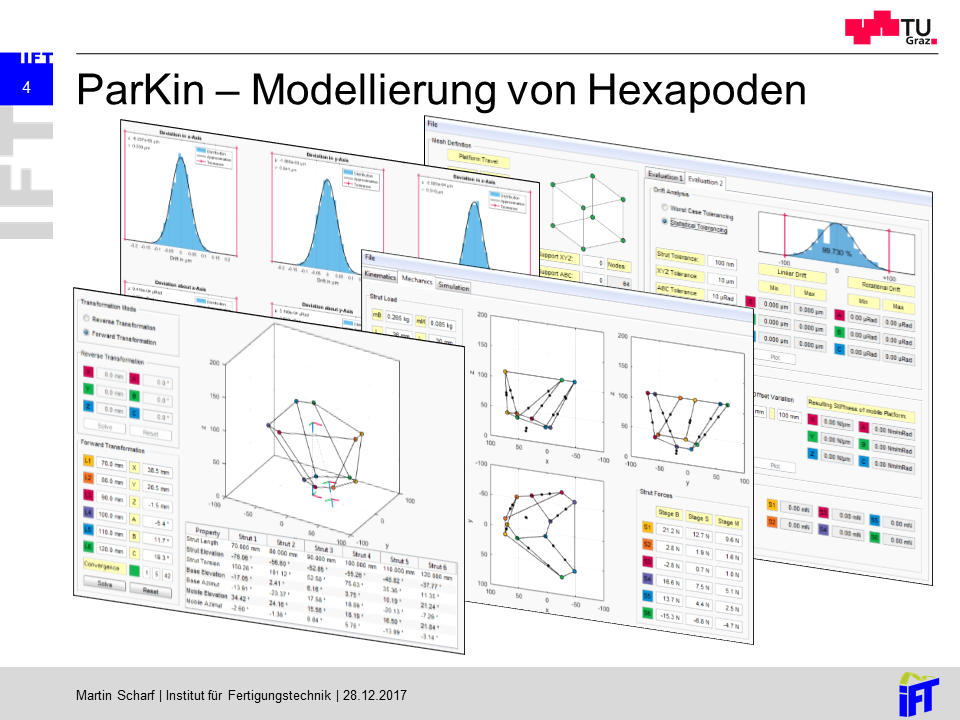
\includegraphics[width=0.7\textwidth]{method/parkin1}
    \caption[Folie]{Folie, Quelle: Eigene Darstellung}
    \label{fig:parkin1}
\end{figure}

\begin{figure}[H]
    \centering
    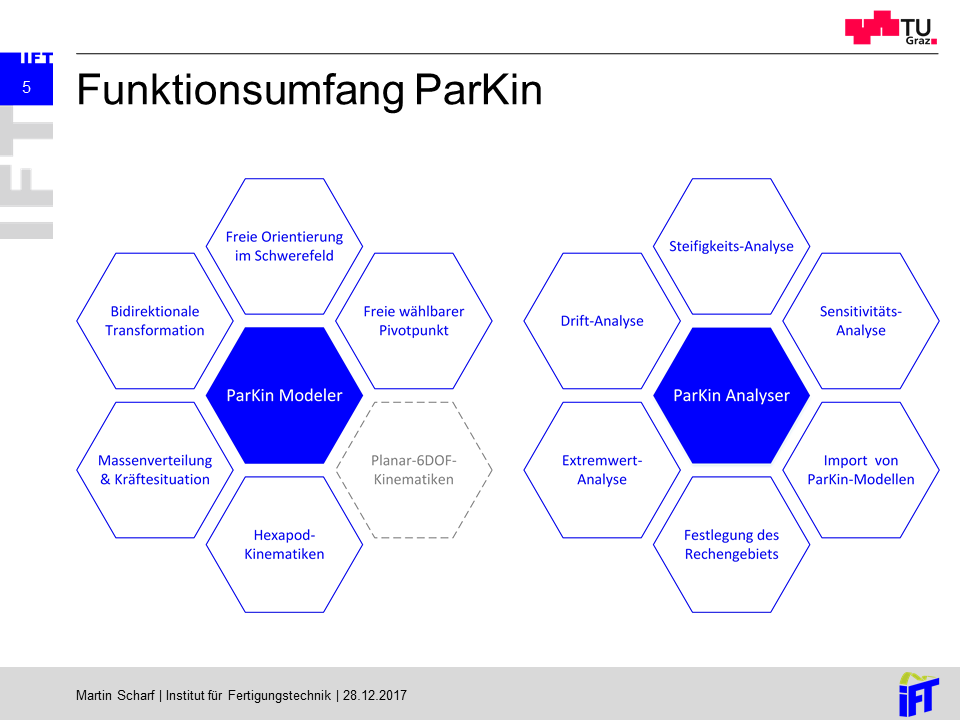
\includegraphics[width=0.7\textwidth]{method/parkin2}
    \caption[Folie]{Folie, Quelle: Eigene Darstellung}
    \label{fig:parkin2}
\end{figure}

\thispagestyle{scrheadings}
\section{Extremwert-Analyse}
\label{method-extreme}

\begin{figure}[H]
    \centering
    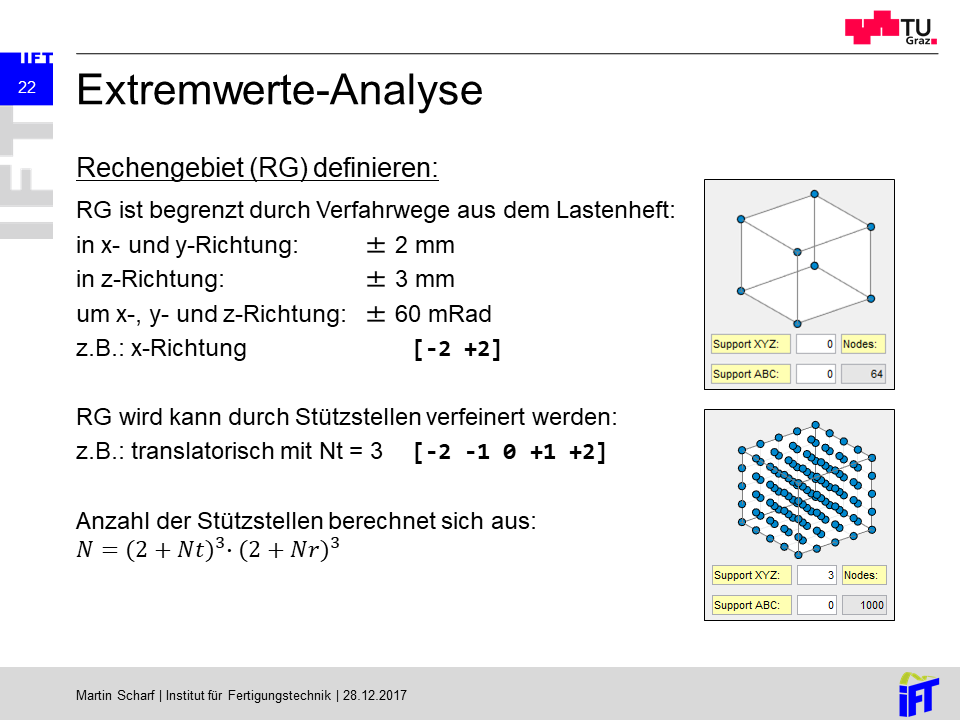
\includegraphics[width=0.7\textwidth]{method/extreme1}
    \caption[Folie]{Folie, Quelle: Eigene Darstellung}
    \label{fig:extreme1}
\end{figure}

\begin{figure}[H]
    \centering
    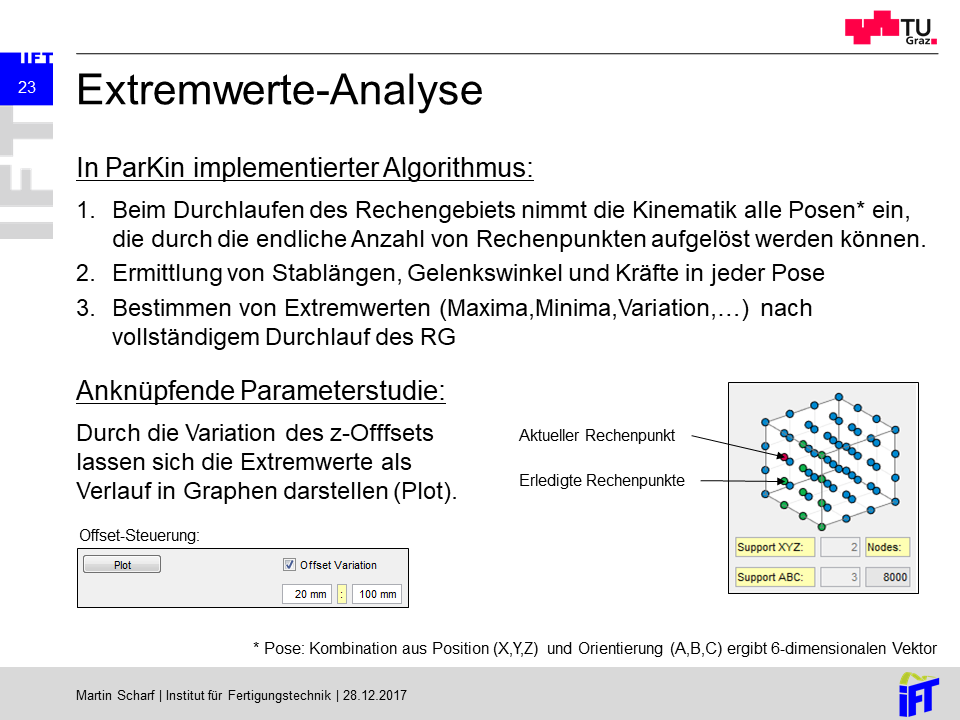
\includegraphics[width=0.7\textwidth]{method/extreme2}
    \caption[Folie]{Folie, Quelle: Eigene Darstellung}
    \label{fig:extreme2}
\end{figure}

\thispagestyle{scrheadings}
\section{Drift-Analyse}
\label{method-drift}

\begin{figure}[H]
    \centering
    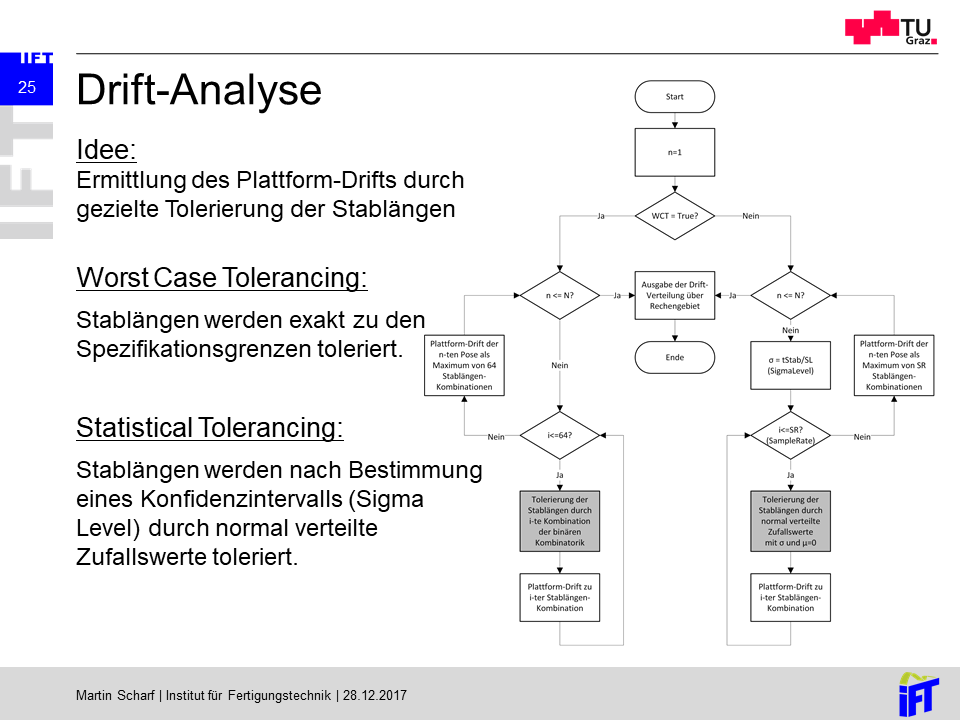
\includegraphics[width=0.7\textwidth]{method/drift1}
    \caption[Folie]{Folie, Quelle: Eigene Darstellung}
    \label{fig:drift1}
\end{figure}

\begin{figure}[H]
    \centering
    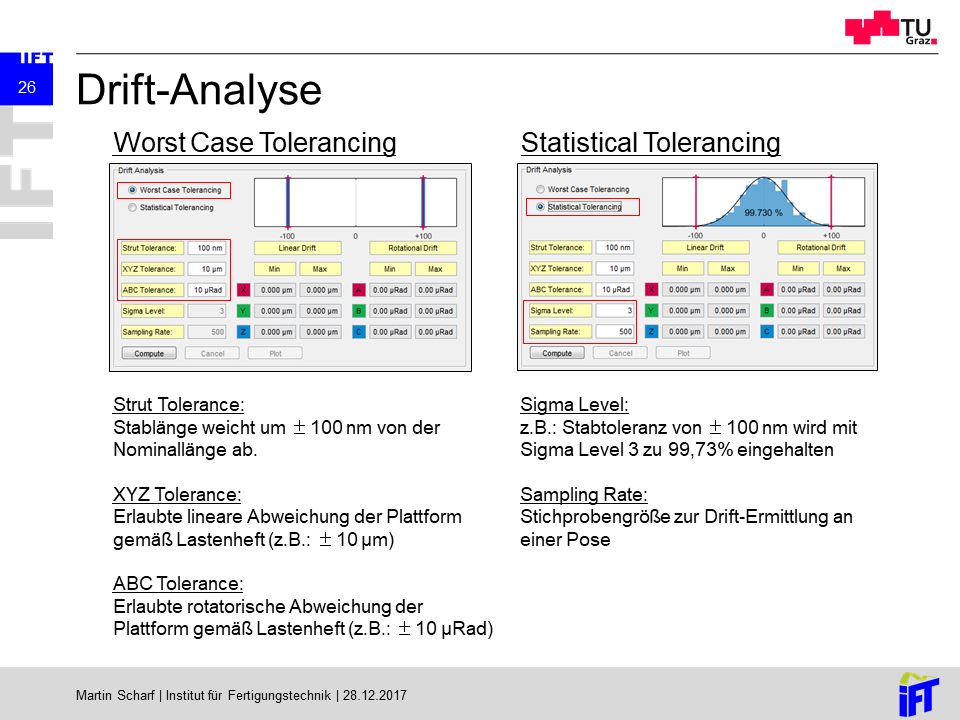
\includegraphics[width=0.7\textwidth]{method/drift2}
    \caption[Folie]{Folie, Quelle: Eigene Darstellung}
    \label{fig:drift2}
\end{figure}

\begin{figure}[H]
    \centering
    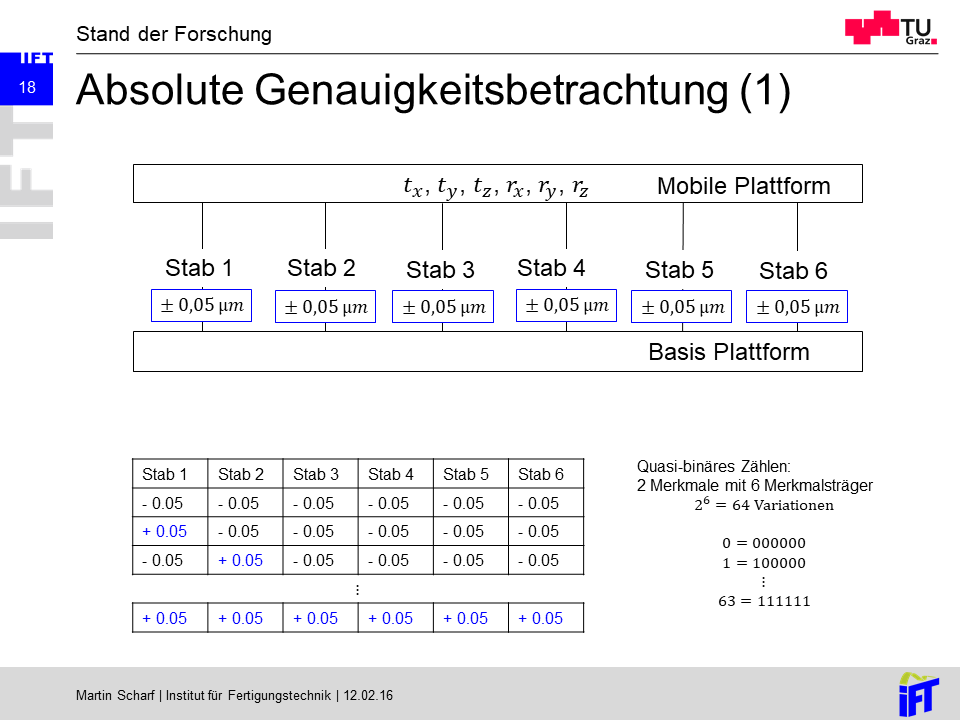
\includegraphics[width=0.7\textwidth]{method/drift3}
    \caption[Folie]{Folie, Quelle: Eigene Darstellung}
    \label{fig:drift3}
\end{figure}

\begin{figure}[H]
    \centering
    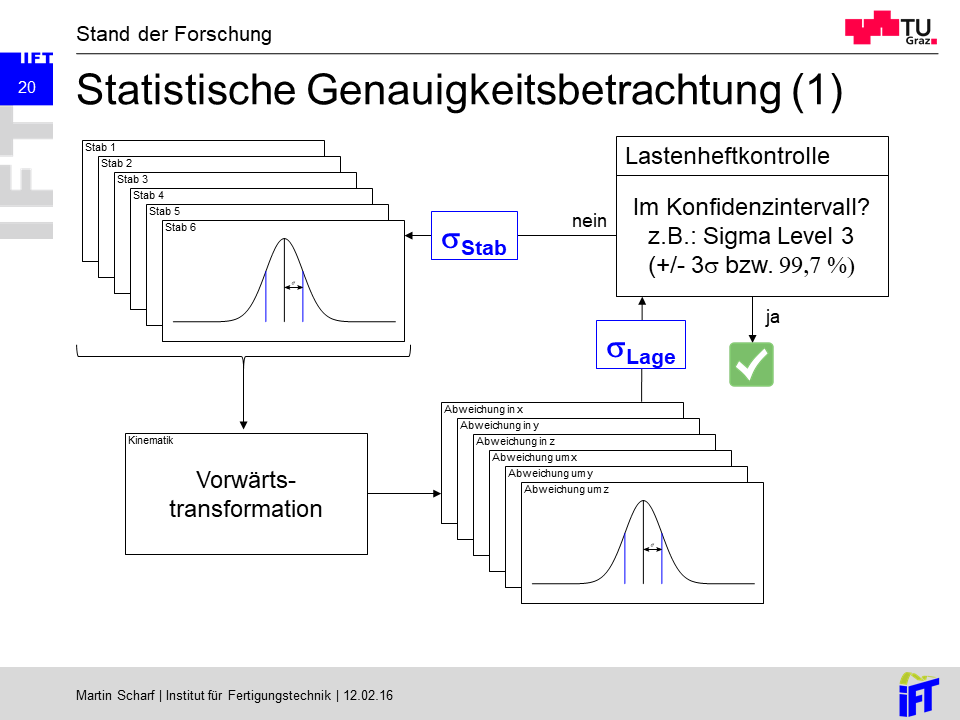
\includegraphics[width=0.7\textwidth]{method/drift4}
    \caption[Folie]{Folie, Quelle: Eigene Darstellung}
    \label{fig:drift4}
\end{figure}

\thispagestyle{scrheadings}
\section{Steifigkeits-Analyse}
\label{method-stiff}

\begin{figure}[H]
    \centering
    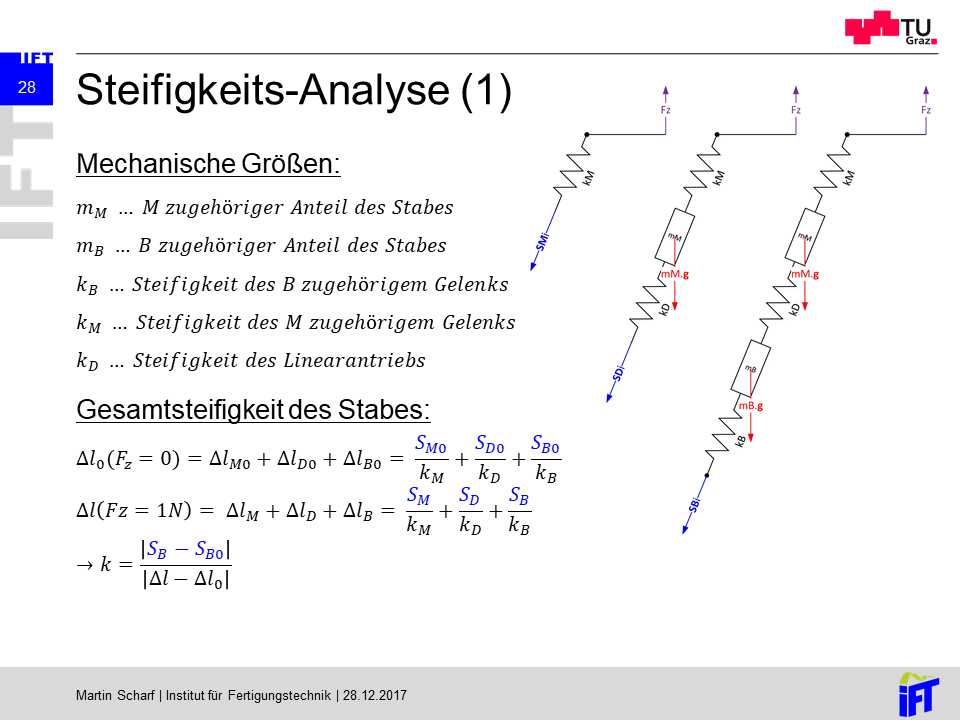
\includegraphics[width=0.7\textwidth]{method/stiff1}
    \caption[Folie]{Folie, Quelle: Eigene Darstellung}
    \label{fig:stiff1}
\end{figure}

\begin{figure}[H]
    \centering
    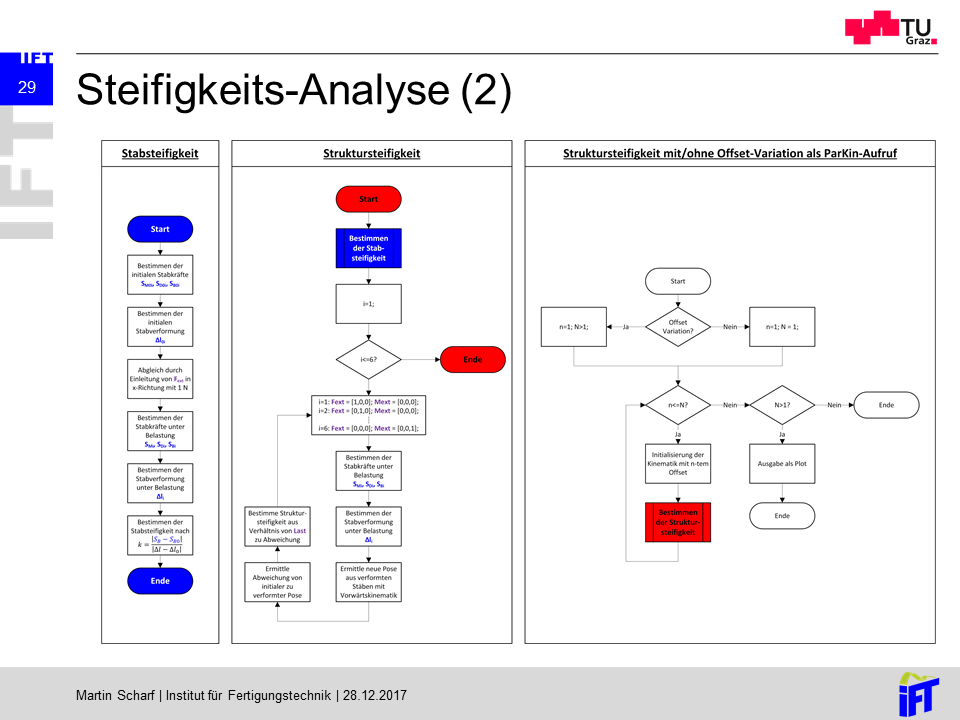
\includegraphics[width=0.7\textwidth]{method/stiff2}
    \caption[Folie]{Folie, Quelle: Eigene Darstellung}
    \label{fig:stiff2}
\end{figure}

\begin{figure}[H]
    \centering
    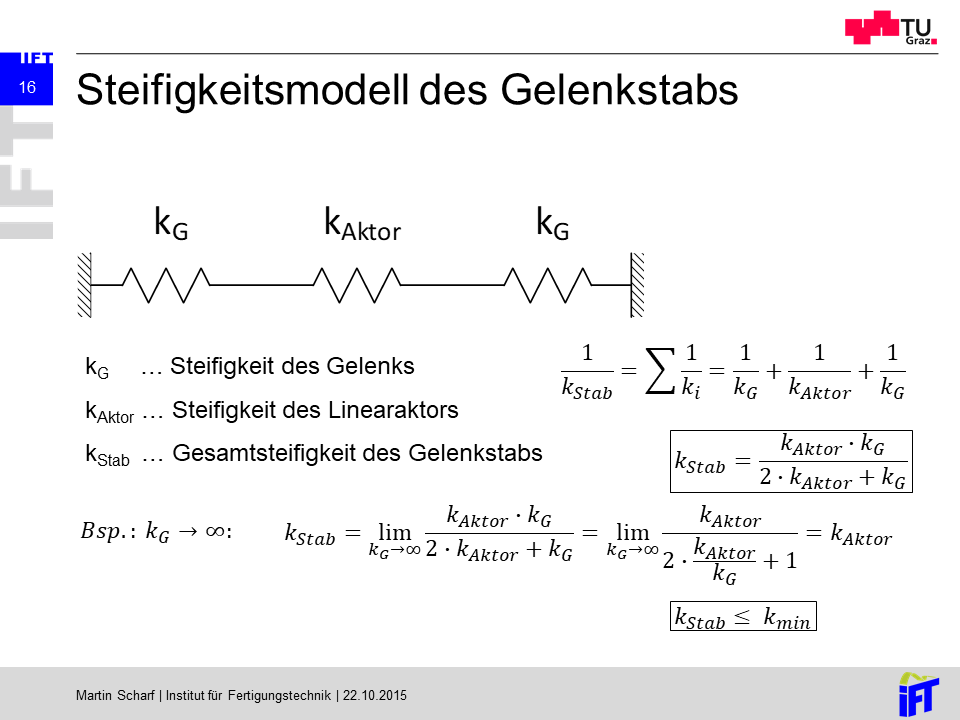
\includegraphics[width=0.7\textwidth]{method/stiff3}
    \caption[Folie]{Folie, Quelle: Eigene Darstellung}
    \label{fig:stiff3}
\end{figure}

\begin{figure}[H]
    \centering
    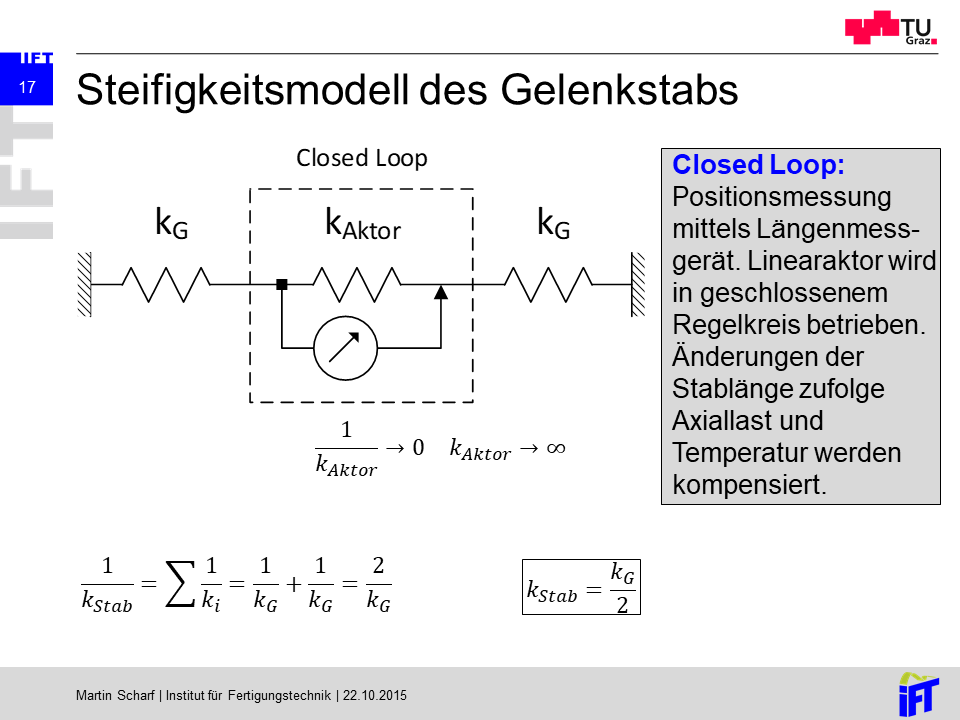
\includegraphics[width=0.7\textwidth]{method/stiff4}
    \caption[Folie]{Folie, Quelle: Eigene Darstellung}
    \label{fig:stiff4}
\end{figure}

\thispagestyle{scrheadings}
\section{Sensitivitätsanalyse-Analyse}
\label{method-sens}

\begin{figure}[H]
    \centering
    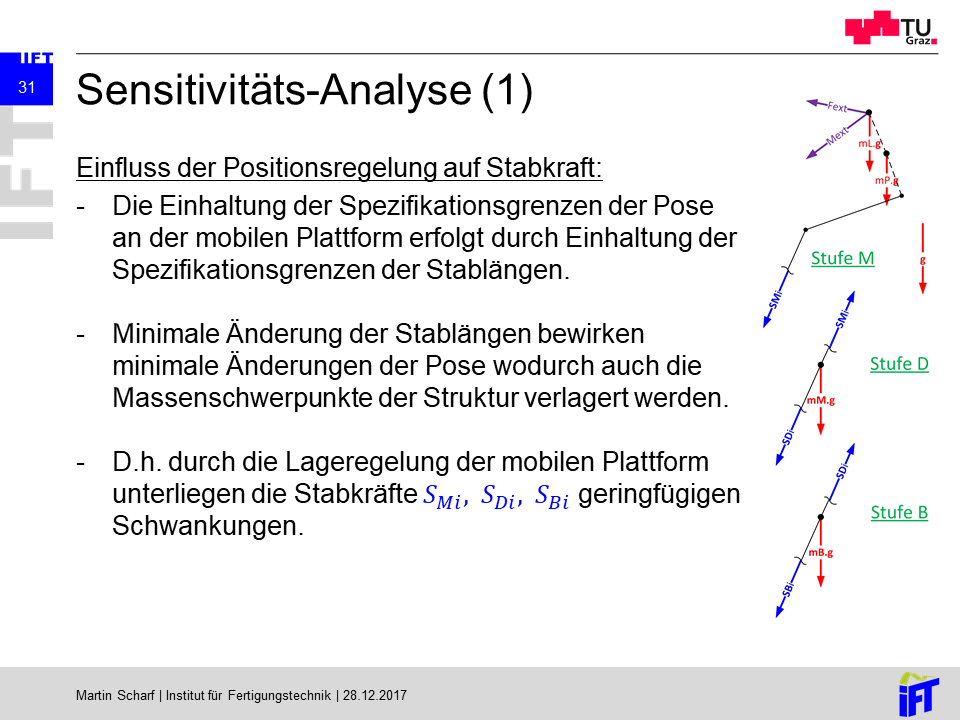
\includegraphics[width=0.7\textwidth]{method/sens1}
    \caption[Folie]{Folie, Quelle: Eigene Darstellung}
    \label{fig:sens1}
\end{figure}

\begin{figure}[H]
    \centering
    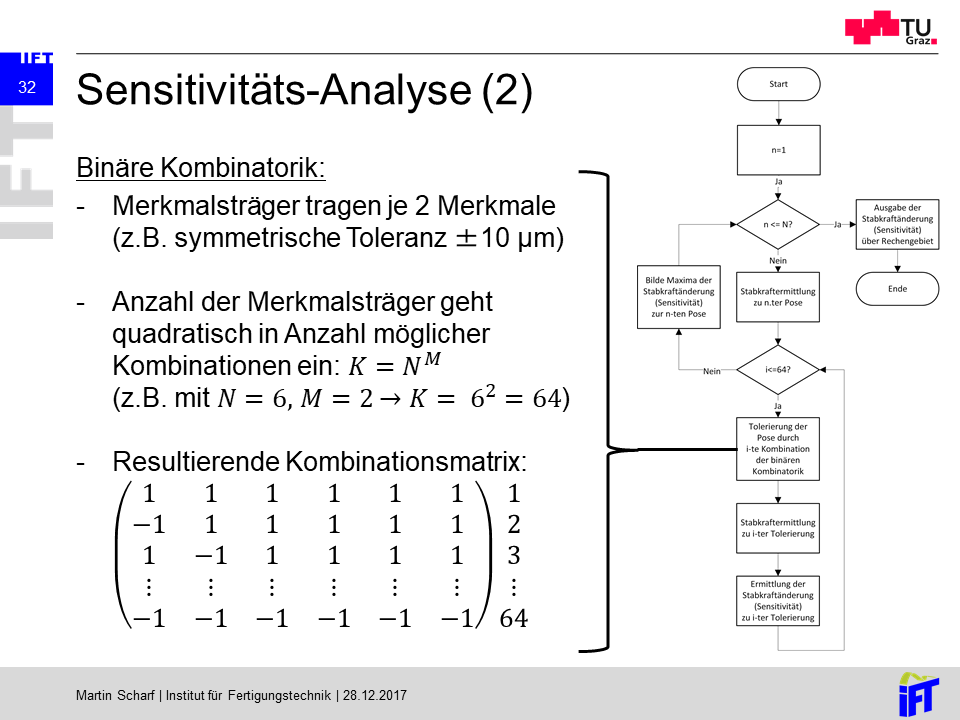
\includegraphics[width=0.7\textwidth]{method/sens2}
    \caption[Folie]{Folie, Quelle: Eigene Darstellung}
    \label{fig:sens2}
\end{figure}

\begin{figure}[H]
    \centering
    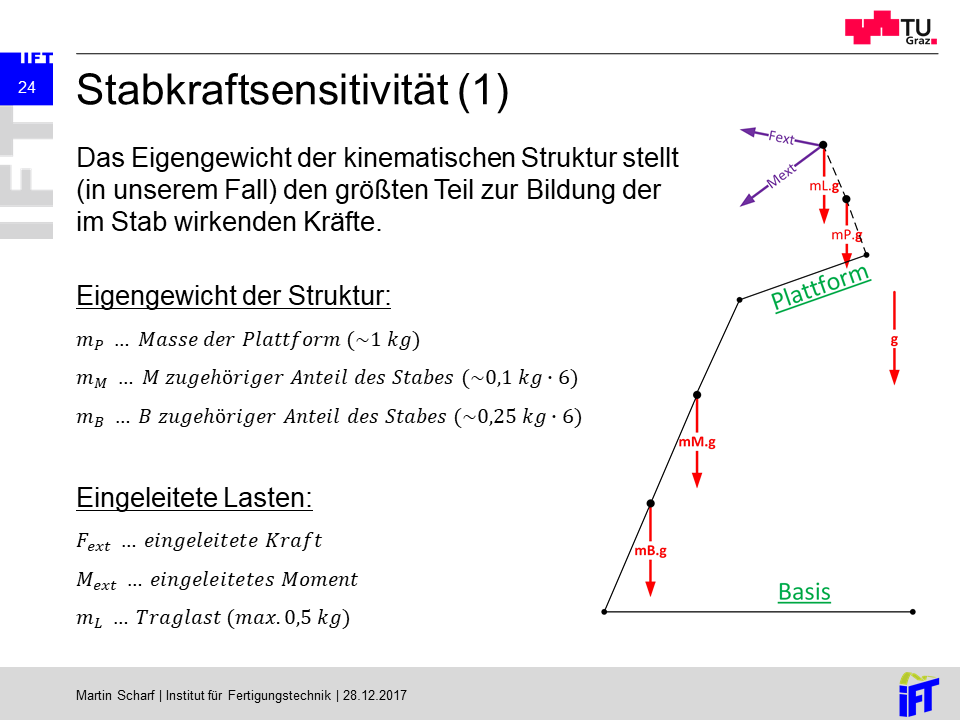
\includegraphics[width=0.7\textwidth]{method/sens3}
    \caption[Folie]{Folie, Quelle: Eigene Darstellung}
    \label{fig:sens3}
\end{figure}

\begin{figure}[H]
    \centering
    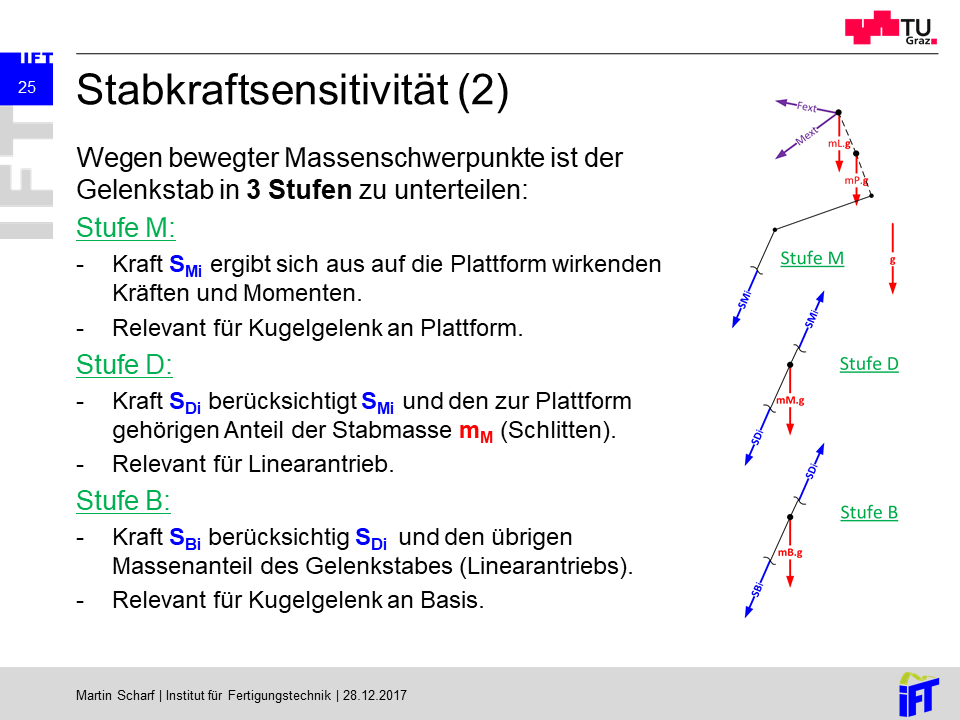
\includegraphics[width=0.7\textwidth]{method/sens4}
    \caption[Folie]{Folie, Quelle: Eigene Darstellung}
    \label{fig:sens4}
\end{figure}
%-----------------------------------------------------------------------------------------------%
\chapter{Ergebnisse}
%%---------------------------------------------------------------------------------------------%
\section{Extremwertmethode}
\label{sec:extreme}
\begin{table}[H]
\centering
\begin{tabularx}{\textwidth}{XccR{\cw}R{\cw}R{\cw}R{\cw}R{\cw}R{\cw}} 
\toprule
Parameter & Symbol & Einheit & \HC{$S_1$} & \HC{$S_2$} & \HC{$S_3$} & \HC{$S_4$} & \HC{$S_5$} & \HC{$S_6$} \\ 
\midrule
Maximallänge  & $\bvec{l}_{i;max}$       & \si{\milli\metre}  & \num{95.326} & \num{95.326} & \num{95.084} & \num{94.996} & \num{94.996} & \num{95.084} \\ 
Minimallänge  & $\bvec{l}_{i;min}$       & \si{\milli\metre}  & \num{79.816} & \num{79.816} & \num{80.222} & \num{80.052} & \num{80.052} & \num{80.222} \\ 
Größtänderung & $\Delta \bvec{l}_i$     & \si{\milli\metre}  & \num{15.510} & \num{15.510} & \num{14.862} & \num{14.944} & \num{14.944} & \num{14.862} \\ 
Größtdehnung  & $\bvec{\varepsilon}_i$  & \si{\percent}  & \num{19.433} & \num{19.433} & \num{18.526} & \num{18.668} & \num{18.668} & \num{18.526} \\ 
\bottomrule
\end{tabularx}
\caption[Extremwerte der Strebenlängen]{Extremwerte der Strebenlängen}
\label{tab:ext_length}
\end{table}
\begin{table}[H]
\centering
\begin{tabularx}{\textwidth}{XccR{\cw}R{\cw}R{\cw}R{\cw}R{\cw}R{\cw}} 
\toprule
Parameter & Symbol & Einheit & \HC{$S_1$} & \HC{$S_2$} & \HC{$S_3$} & \HC{$S_4$} & \HC{$S_5$} & \HC{$S_6$} \\ 
\midrule
Höhenwinkel  & $\vartheta_{Bi}$ & \si{\degree} & \num{2.828} & \num{2.828} & \num{3.005} & \num{2.723} & \num{2.723} & \num{3.005} \\ 
Azimutwinkel & $\varphi_{Bi}$   & \si{\degree} & \num{4.892} & \num{4.892} & \num{4.886} & \num{4.750} & \num{4.750} & \num{4.886} \\ 
Gelenkwinkel & $\psi_{Bi}$      & \si{\degree} & \num{5.135} & \num{5.135} & \num{4.936} & \num{4.901} & \num{4.901} & \num{4.936} \\ 
\bottomrule
\end{tabularx}
\caption[Extremwerte der Gelenkwinkel an der Basis]{Extremwerte der Gelenkwinkel an der Basis}
\label{tab:tab_ext_angle_b}
\end{table}
\begin{table}[H]
\centering
\begin{tabularx}{\textwidth}{XccR{\cw}R{\cw}R{\cw}R{\cw}R{\cw}R{\cw}} 
\toprule
Parameter & Symbol & Einheit & \HC{$S_1$} & \HC{$S_2$} & \HC{$S_3$} & \HC{$S_4$} & \HC{$S_5$} & \HC{$S_6$} \\ 
\midrule
Höhenwinkel  & $\vartheta_{Pi}$ & \si{\degree} & \num{2.949} & \num{2.949} & \num{3.060} & \num{2.756} & \num{2.756} & \num{3.060} \\ 
Azimutwinkel & $\varphi_{Pi}$   & \si{\degree} & \num{4.832} & \num{4.832} & \num{4.886} & \num{4.741} & \num{4.741} & \num{4.886} \\ 
Gelenkwinkel & $\psi_{Pi}$      & \si{\degree} & \num{5.135} & \num{5.135} & \num{4.936} & \num{4.901} & \num{4.901} & \num{4.936} \\ 
\bottomrule
\end{tabularx}
\caption[Extremwerte der Gelenkwinkel an der Plattform]{Extremwerte der Gelenkwinkel an der Plattform}
\label{tab:tab_ext_angle_b}
\end{table}
\begin{table}[H]
\centering
\begin{tabularx}{\textwidth}{XccR{\cw}R{\cw}R{\cw}R{\cw}R{\cw}R{\cw}} 
\toprule
Parameter & Symbol & Einheit & \HC{$S_1$} & \HC{$S_2$} & \HC{$S_3$} & \HC{$S_4$} & \HC{$S_5$} & \HC{$S_6$} \\ 
\midrule
Verwindung & $\xi_i$ & \si{\degree}  & \num{4.019} & \num{4.019} & \num{4.438} & \num{3.922} & \num{3.922} & \num{4.438} \\ 
\bottomrule
\end{tabularx}
\caption[Extremwerte der Strebenverwindung]{Extremwerte der Strebenverwindung}
\label{tab:tab_ext_angle_t}
\end{table}
\begin{table}[H]
\centering
\begin{tabularx}{\textwidth}{XccR{\cw}R{\cw}R{\cw}R{\cw}R{\cw}R{\cw}} 
\toprule
Parameter & Symbol & Einheit & \HC{$S_1$} & \HC{$S_2$} & \HC{$S_3$} & \HC{$S_4$} & \HC{$S_5$} & \HC{$S_6$} \\ 
\midrule
Maximalkraft  & $\bvec{F}_{Bi;max}$          & \si{\newton}  & \num{-2.705} & \num{-2.705} & \num{-2.769} & \num{-2.590} & \num{-2.590} & \num{-2.769} \\ 
Minimalkraft  & $\bvec{F}_{Bi;min}$          & \si{\newton}  & \num{-5.712} & \num{-5.712} & \num{-5.730} & \num{-5.776} & \num{-5.776} & \num{-5.730} \\ 
Mittelkraft   & $\overline{\bvec{F}_{Bi}}$  & \si{\newton}  & \num{-4.208} & \num{-4.208} & \num{-4.249} & \num{-4.183} & \num{-4.183} & \num{-4.249} \\ 
Kraftänderung & $\Delta\bvec{F}_{Bi}$       & \si{\newton}  & \num{3.007} & \num{3.007} & \num{2.961} & \num{3.186} & \num{3.186} & \num{2.961} \\ 
\bottomrule
\end{tabularx}
\caption[Extremwerte der Strebenkräfte an der Basis]{Extremwerte der Strebenkräfte an der Basis}
\label{tab:ext_force_b}
\end{table}
\begin{table}[H]
\centering
\begin{tabularx}{\textwidth}{XccR{\cw}R{\cw}R{\cw}R{\cw}R{\cw}R{\cw}} 
\toprule
Parameter & Symbol & Einheit & \HC{$S_1$} & \HC{$S_2$} & \HC{$S_3$} & \HC{$S_4$} & \HC{$S_5$} & \HC{$S_6$} \\ 
\midrule
Maximalkraft  & $\bvec{F}_{Pi;max}$          & \si{\newton}  & \num{-1.207} & \num{-1.207} & \num{-1.167} & \num{-1.150} & \num{-1.150} & \num{-1.167} \\ 
Minimalkraft  & $\bvec{F}_{Pi;min}$          & \si{\newton}  & \num{-2.680} & \num{-2.680} & \num{-2.643} & \num{-2.651} & \num{-2.651} & \num{-2.643} \\ 
Mittelkraft   & $\overline{\bvec{F}_{Pi}}$  & \si{\newton}  & \num{-1.944} & \num{-1.944} & \num{-1.905} & \num{-1.901} & \num{-1.901} & \num{-1.905} \\ 
Kraftänderung & $\Delta\bvec{F}_{Pi}$       & \si{\newton}  & \num{1.473} & \num{1.473} & \num{1.475} & \num{1.501} & \num{1.501} & \num{1.475} \\ 
\bottomrule
\end{tabularx}
\caption[Extremwerte der Strebenkräfte an der Plattform]{Extremwerte der Strebenkräfte an der Plattform}
\label{tab:ext_force_p}
\end{table}
\begin{table}[H]
\centering
\begin{tabularx}{\textwidth}{XccR{\cw}R{\cw}R{\cw}R{\cw}R{\cw}R{\cw}} 
\toprule
Parameter & Symbol & Einheit & \HC{$S_1$} & \HC{$S_2$} & \HC{$S_3$} & \HC{$S_4$} & \HC{$S_5$} & \HC{$S_6$} \\ 
\midrule
Maximalkraft  & $\bvec{F}_{Li;max}$          & \si{\newton}  & \num{-1.988} & \num{-1.988} & \num{-1.981} & \num{-1.917} & \num{-1.917} & \num{-1.981} \\ 
Minimalkraft  & $\bvec{F}_{Li;min}$          & \si{\newton}  & \num{-4.180} & \num{-4.180} & \num{-4.129} & \num{-4.170} & \num{-4.170} & \num{-4.129} \\ 
Mittelkraft   & $\overline{\bvec{F}_{Li}}$  & \si{\newton}  & \num{-3.084} & \num{-3.084} & \num{-3.055} & \num{-3.043} & \num{-3.043} & \num{-3.055} \\ 
Kraftänderung & $\Delta\bvec{F}_{Li}$       & \si{\newton}  & \num{2.192} & \num{2.192} & \num{2.148} & \num{2.253} & \num{2.253} & \num{2.148} \\ 
\bottomrule
\end{tabularx}
\caption[Extremwerte der Strebenkräfte am Linearversteller]{Extremwerte der Strebenkräfte am Linearversteller}
\label{tab:ext_force_l}
\end{table}
%---------------------------------------------------------------------------------------------%

%---------------------------------------------------------------------------------------------%
\section{Abweichungsanalyse}
\label{sec:drift}
\newpage
\blindtext[1]
\begin{figure}[H]
    \centering
    \begin{subfigure}[b]{\textwidth}
    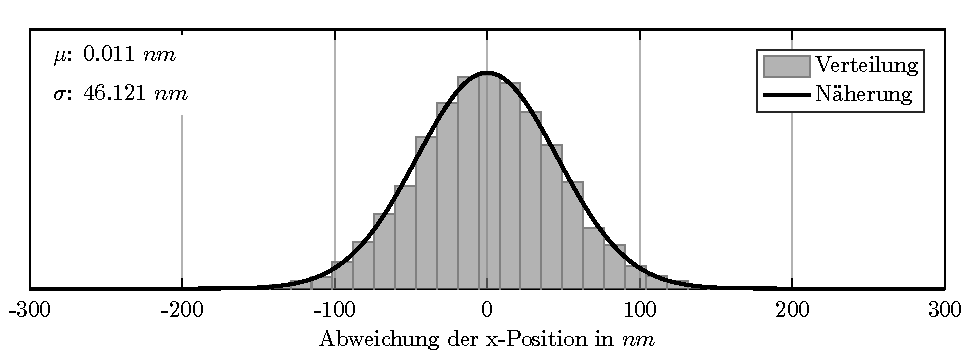
\includegraphics{graphics/results/drift/fig_drift_axis_tx.pdf}
    \end{subfigure}
    \begin{subfigure}[b]{\textwidth}
    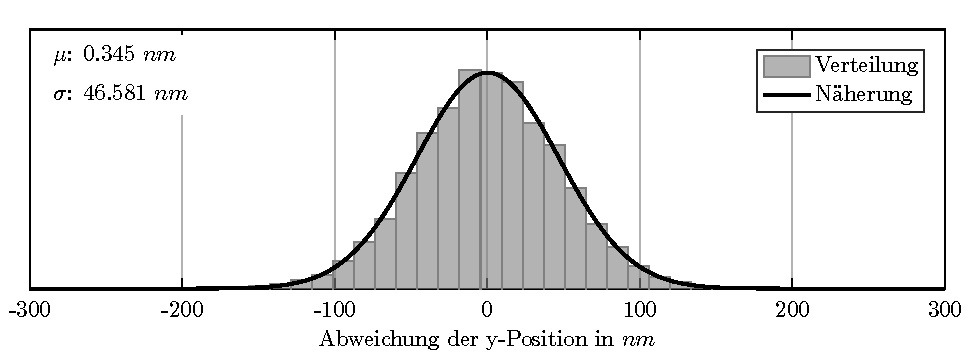
\includegraphics{graphics/results/drift/fig_drift_axis_ty.pdf}
    \end{subfigure}
    \begin{subfigure}[b]{\textwidth}
    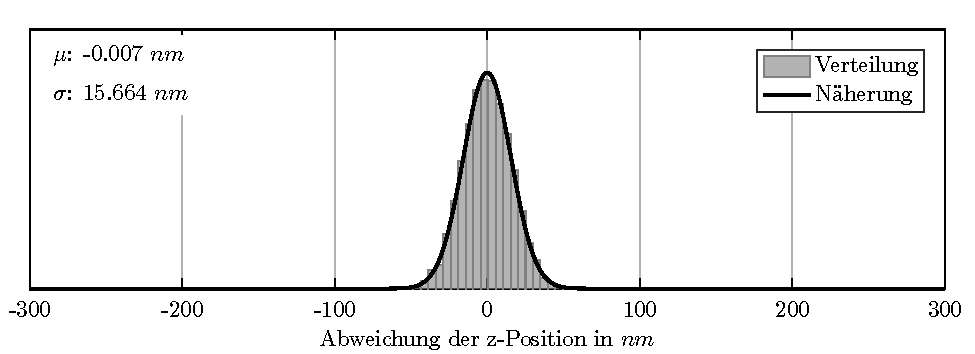
\includegraphics{graphics/results/drift/fig_drift_axis_tz.pdf}
    \end{subfigure}
    \caption[Abweichung der Plattformposition]{Abweichung der Plattformposition}\label{fig:results_drift_t}
\end{figure}
\blindtext[1]
\begin{figure}[H]
    \centering
    \begin{subfigure}[b]{\textwidth}
    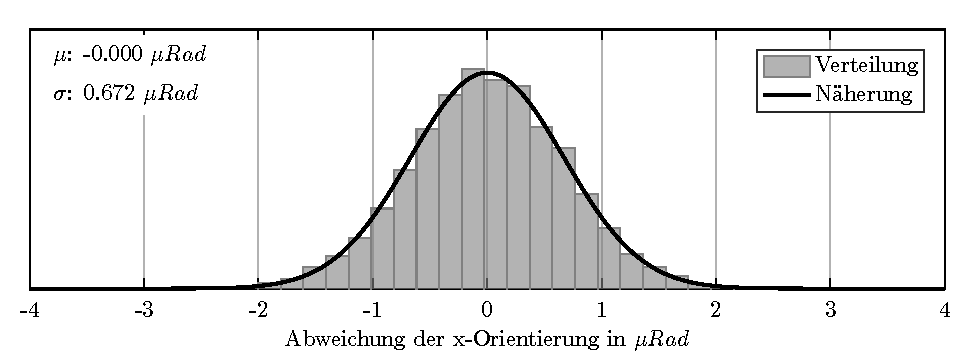
\includegraphics{graphics/results/drift/fig_drift_axis_rx.pdf}
    \end{subfigure}
    \begin{subfigure}[b]{\textwidth}
    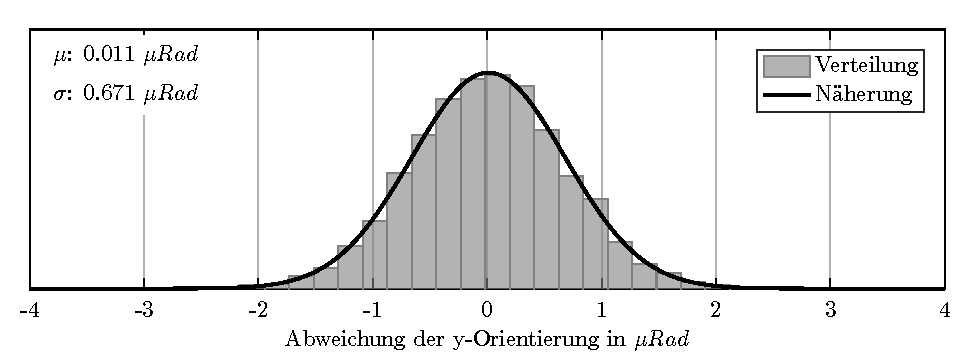
\includegraphics{graphics/results/drift/fig_drift_axis_ry.pdf}
    \end{subfigure}
    \begin{subfigure}[b]{\textwidth}
    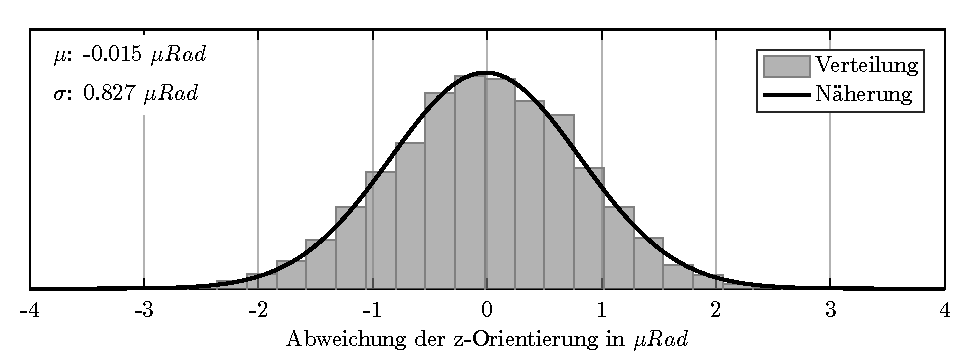
\includegraphics{graphics/results/drift/fig_drift_axis_rz.pdf}
    \end{subfigure}
    \caption[Abweichung der Plattformorientierung]{Abweichung der Plattformorientierung}\label{fig:results_drift_r}
\end{figure}
\blindtext[1]
%---------------------------------------------------------------------------------------------%
%-----------------------------------------------------------------------------------------------%
\chapter{Diskussion}
%\thispagestyle{scrheadings}
\section{Vergleich mit anderen Hexapoden}
\label{disc-comp}

\begin{figure}[H]
    \centering
    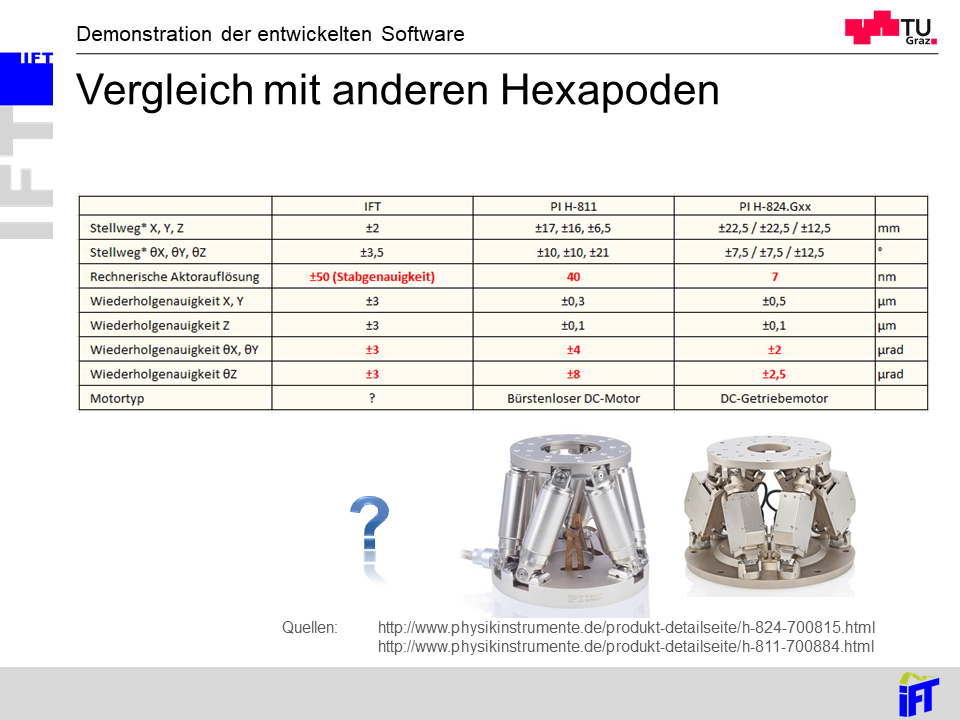
\includegraphics[width=0.7\textwidth]{disc/comp}
    \caption[Folie]{Folie, Quelle: Eigene Darstellung}
    \label{fig:comp}
\end{figure}

\thispagestyle{scrheadings}
\section{Anforderungen an die Messtechnik}
\label{disc-mess}

\begin{figure}[H]
    \centering
    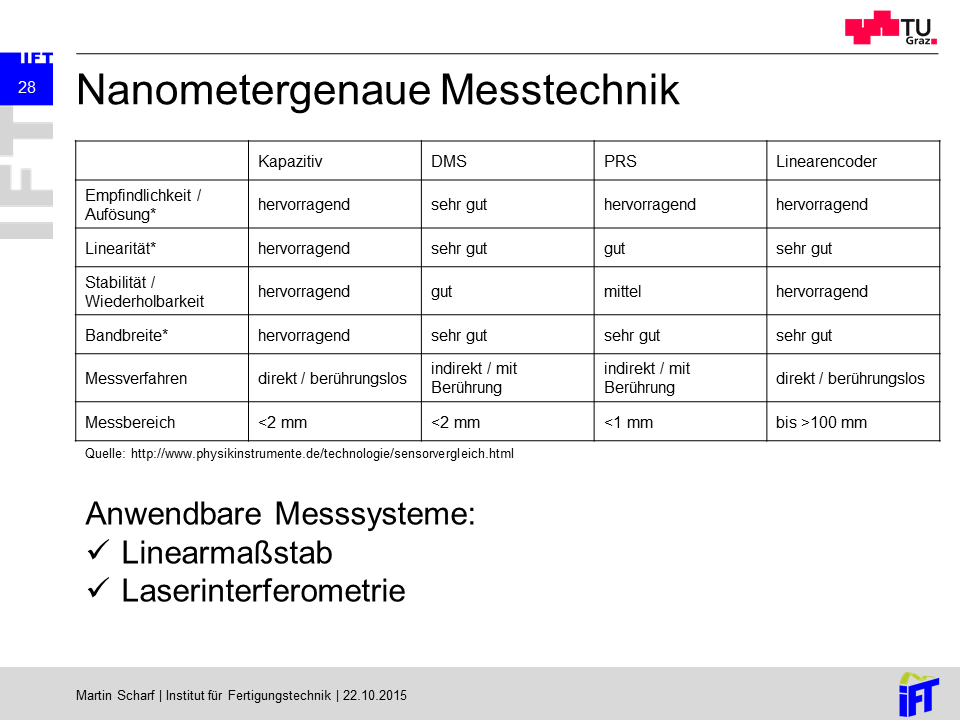
\includegraphics[width=0.7\textwidth]{disc/mess1}
    \caption[Folie]{Folie, Quelle: Eigene Darstellung}
    \label{fig:mess1}
\end{figure}

\begin{figure}[H]
    \centering
    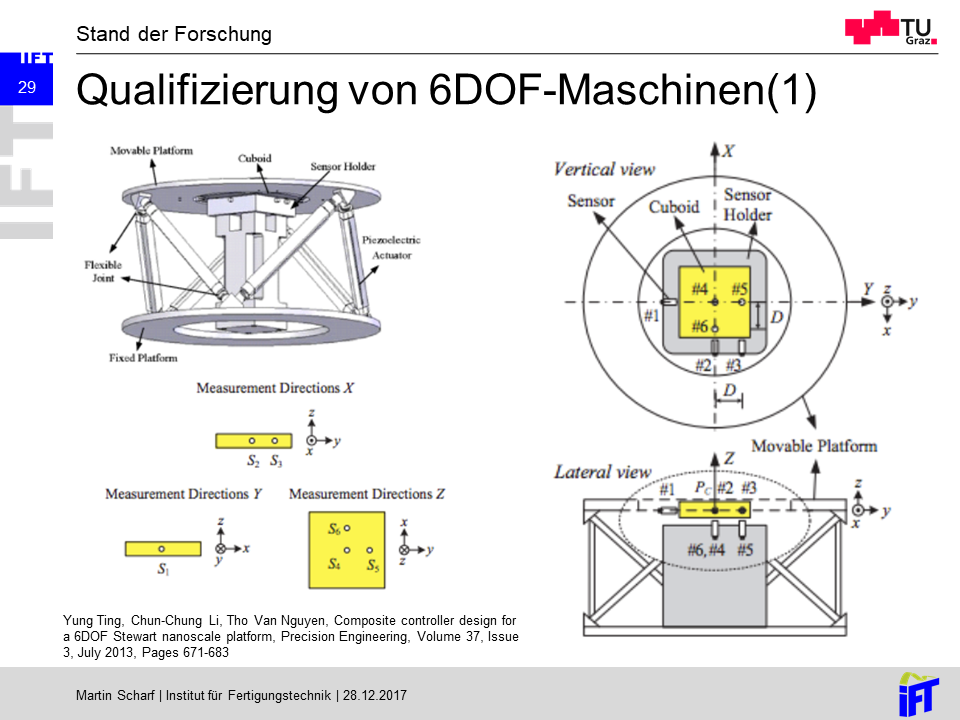
\includegraphics[width=0.7\textwidth]{disc/mess2}
    \caption[Folie]{Folie, Quelle: Eigene Darstellung}
    \label{fig:mess2}
\end{figure}

\begin{figure}[H]
    \centering
    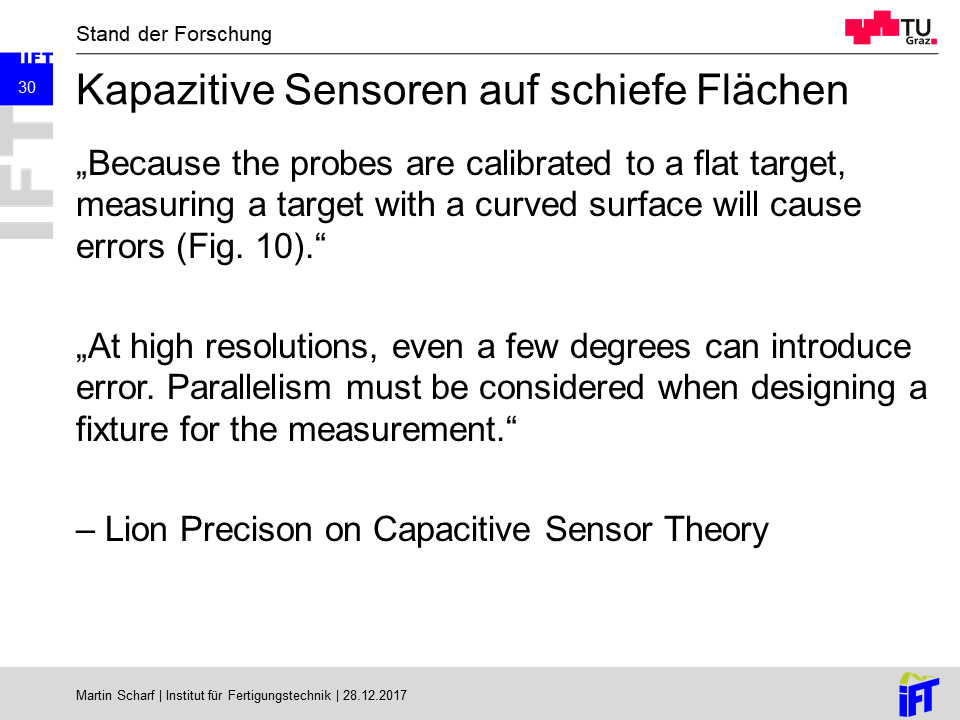
\includegraphics[width=0.7\textwidth]{disc/mess3}
    \caption[Folie]{Folie, Quelle: Eigene Darstellung}
    \label{fig:mess3}
\end{figure}

\begin{figure}[H]
    \centering
    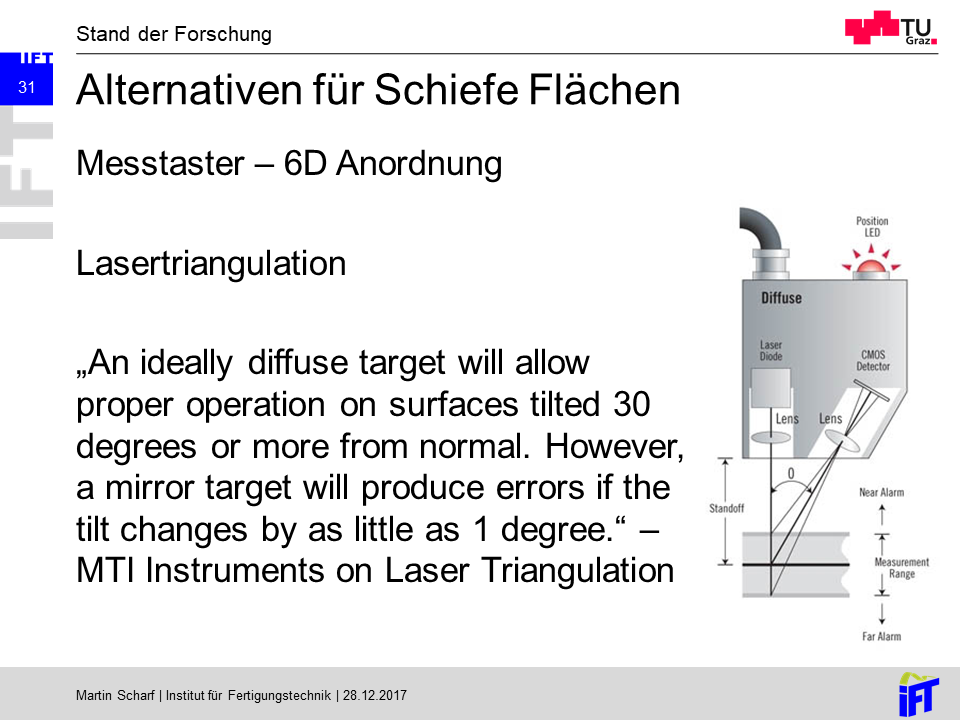
\includegraphics[width=0.7\textwidth]{disc/mess4}
    \caption[Folie]{Folie, Quelle: Eigene Darstellung}
    \label{fig:mess4}
\end{figure}

\begin{figure}[H]
    \centering
    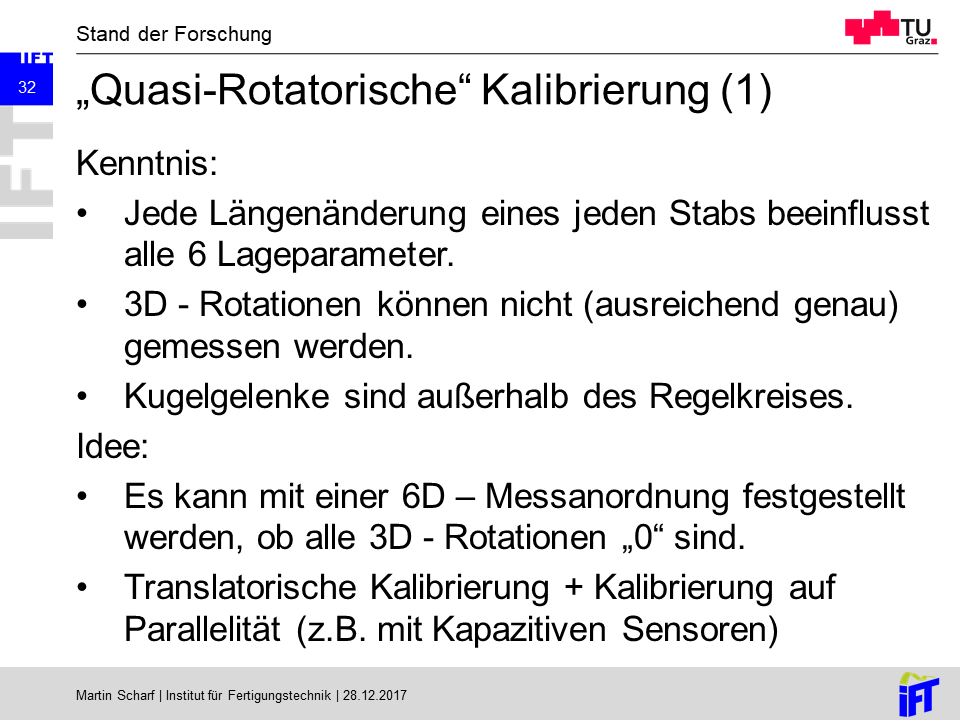
\includegraphics[width=0.7\textwidth]{disc/mess5}
    \caption[Folie]{Folie, Quelle: Eigene Darstellung}
    \label{fig:mess5}
\end{figure}

\begin{figure}[H]
    \centering
    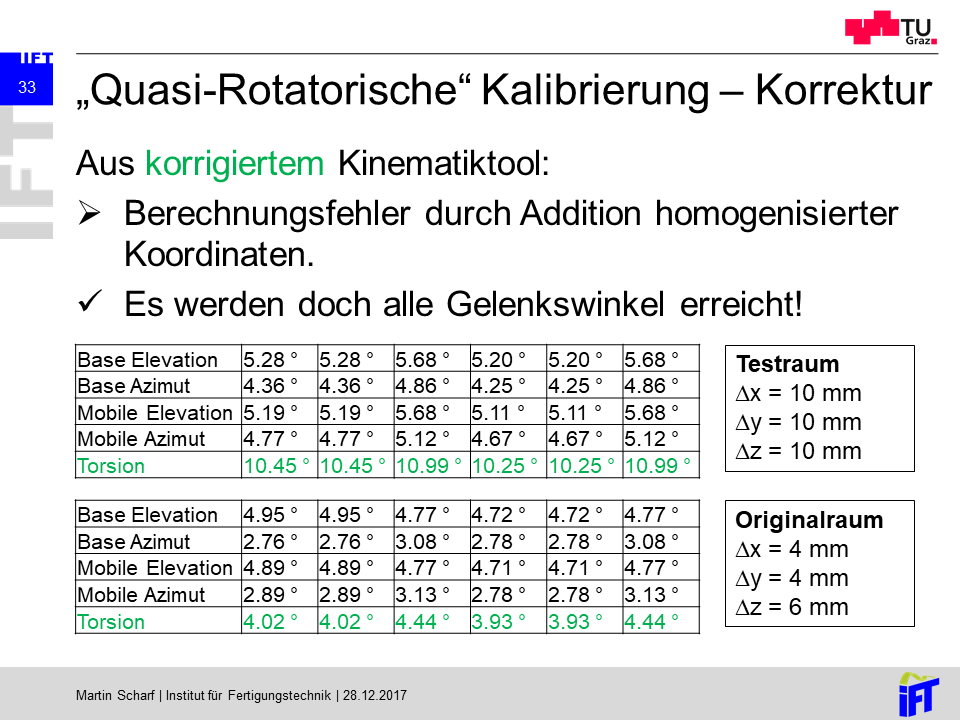
\includegraphics[width=0.7\textwidth]{disc/mess6}
    \caption[Folie]{Folie, Quelle: Eigene Darstellung}
    \label{fig:mess6}
\end{figure}

\begin{figure}[H]
    \centering
    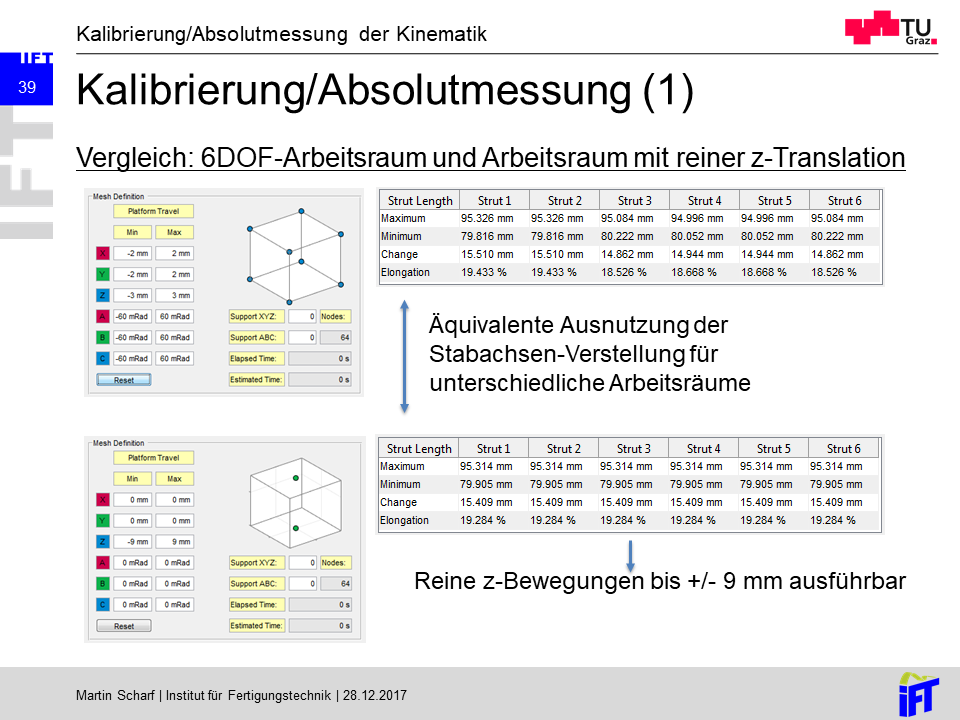
\includegraphics[width=0.7\textwidth]{disc/mess7}
    \caption[Folie]{Folie, Quelle: Eigene Darstellung}
    \label{fig:mess7}
\end{figure}

\begin{figure}[H]
    \centering
    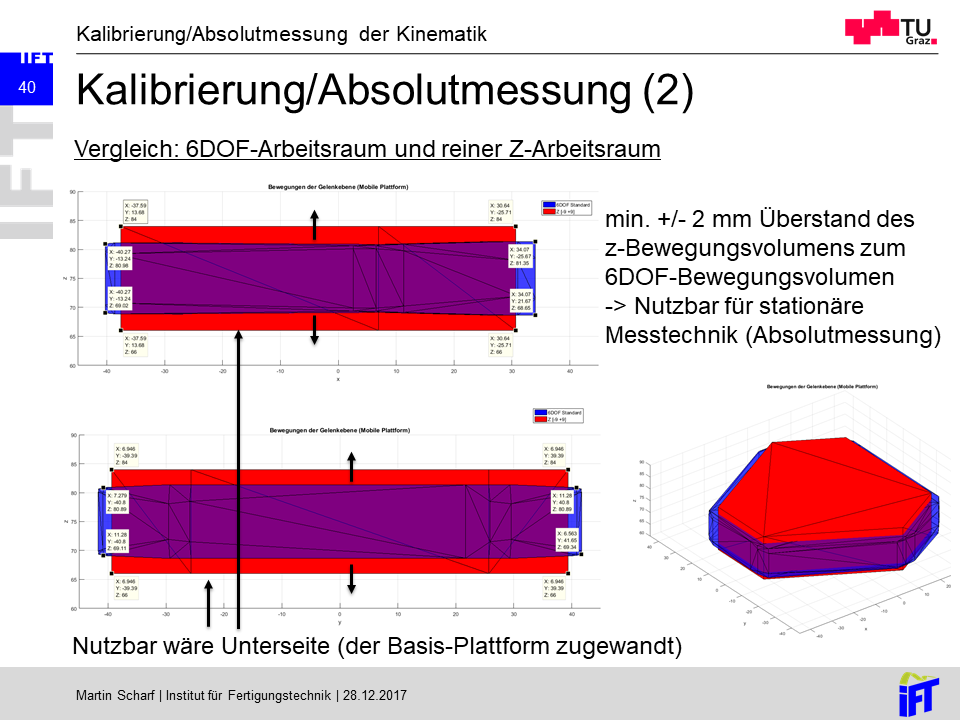
\includegraphics[width=0.7\textwidth]{disc/mess8}
    \caption[Folie]{Folie, Quelle: Eigene Darstellung}
    \label{fig:mess8}
\end{figure}

\begin{figure}[H]
    \centering
    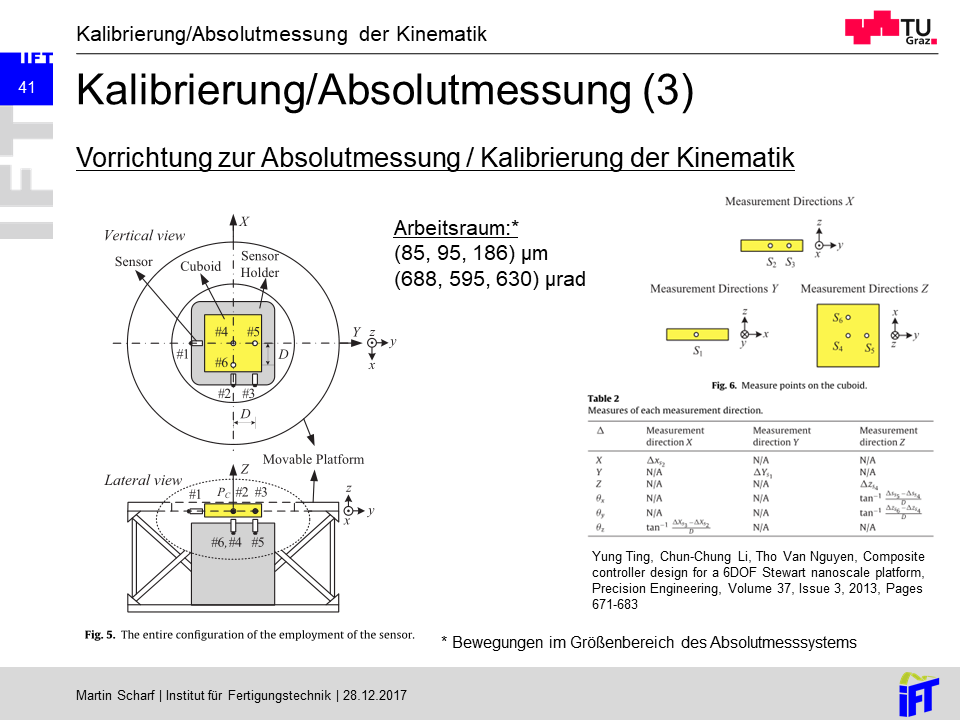
\includegraphics[width=0.7\textwidth]{disc/mess9}
    \caption[Folie]{Folie, Quelle: Eigene Darstellung}
    \label{fig:mess9}
\end{figure}

\thispagestyle{scrheadings}
\section{Werkstoffwahl}
\label{disc-mess}

\begin{figure}[H]
    \centering
    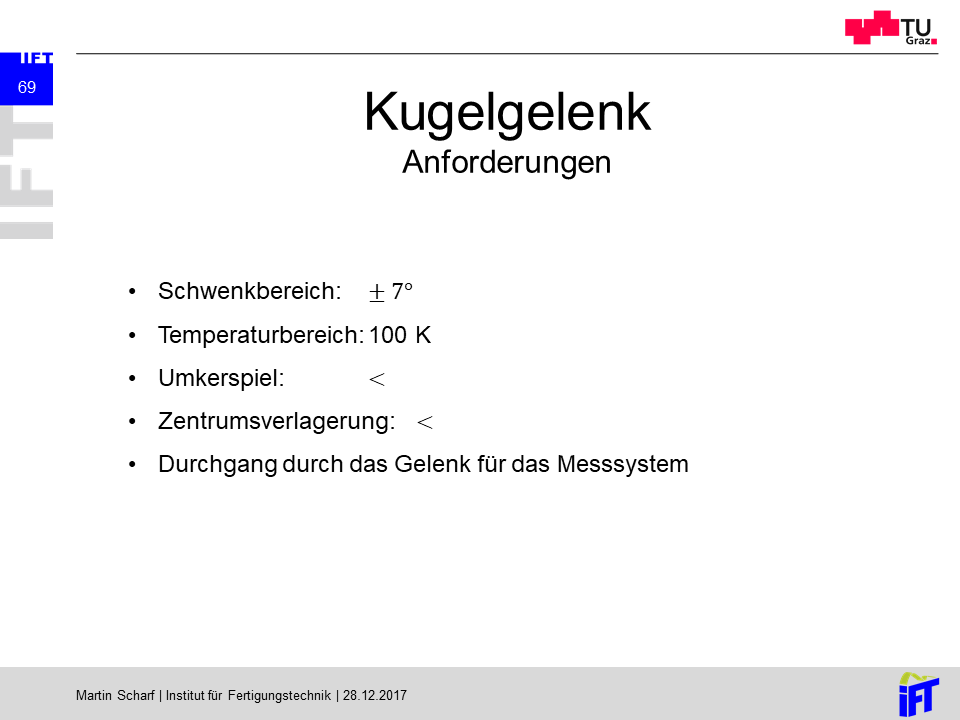
\includegraphics[width=0.7\textwidth]{disc/ws1}
    \caption[Folie]{Folie, Quelle: Eigene Darstellung}
    \label{fig:ws1}
\end{figure}

\begin{figure}[H]
    \centering
    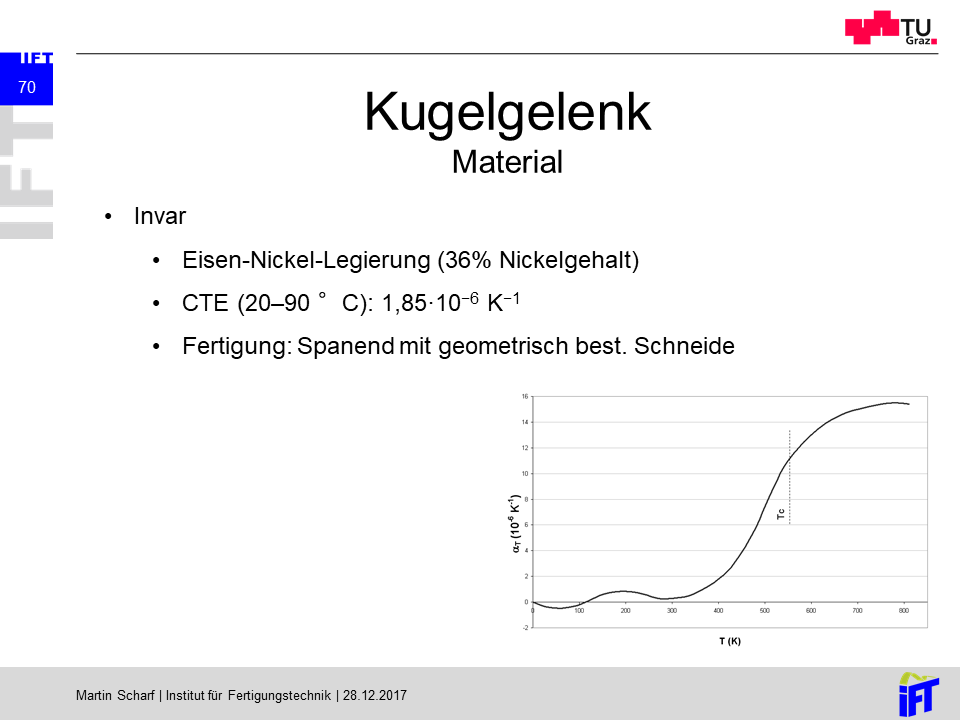
\includegraphics[width=0.7\textwidth]{disc/ws2}
    \caption[Folie]{Folie, Quelle: Eigene Darstellung}
    \label{fig:ws2}
\end{figure}

\begin{figure}[H]
    \centering
    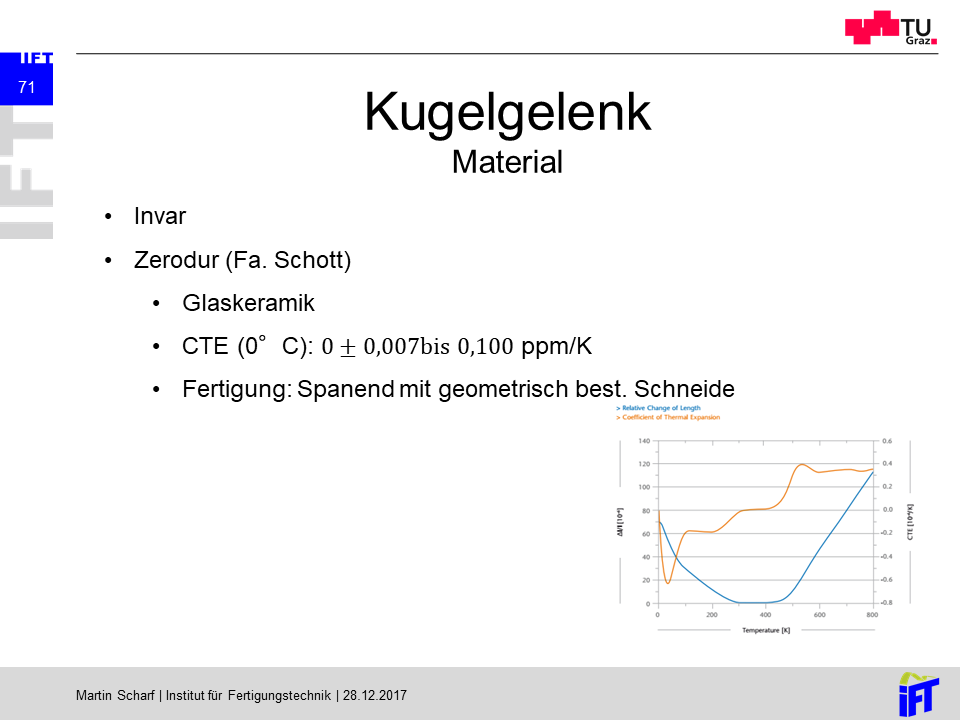
\includegraphics[width=0.7\textwidth]{disc/ws3}
    \caption[Folie]{Folie, Quelle: Eigene Darstellung}
    \label{fig:ws3}
\end{figure}

\begin{figure}[H]
    \centering
    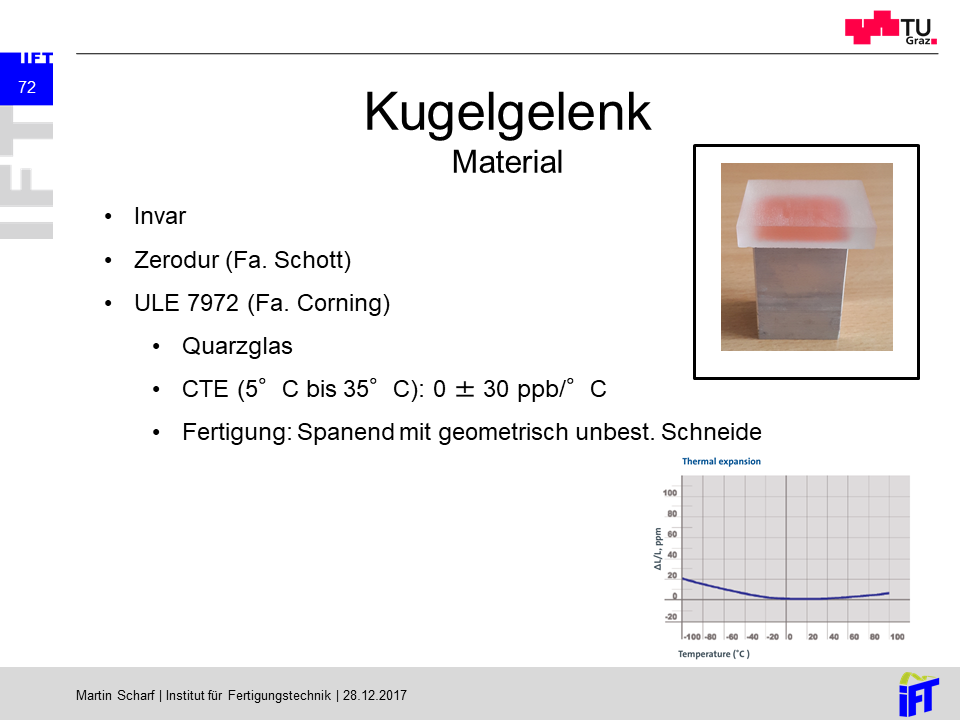
\includegraphics[width=0.7\textwidth]{disc/ws4}
    \caption[Folie]{Folie, Quelle: Eigene Darstellung}
    \label{fig:ws4}
\end{figure}

\begin{figure}[H]
    \centering
    \includegraphics[width=0.7\textwidth]{disc/ws5}
    \caption[Folie]{Folie, Quelle: Eigene Darstellung}
    \label{fig:ws5}
\end{figure}

\begin{figure}[H]
    \centering
    \includegraphics[width=0.7\textwidth]{disc/ws6}
    \caption[Folie]{Folie, Quelle: Eigene Darstellung}
    \label{fig:ws6}
\end{figure}

\begin{figure}[H]
    \centering
    \includegraphics[width=0.7\textwidth]{disc/ws7}
    \caption[Folie]{Folie, Quelle: Eigene Darstellung}
    \label{fig:ws7}
\end{figure}

\thispagestyle{scrheadings}
\section{Anforderungen an die Antriebstechnik}
\label{disc-mess}

\begin{figure}[H]
    \centering
    \includegraphics[width=0.7\textwidth]{disc/mech1}
    \caption[Folie]{Folie, Quelle: Eigene Darstellung}
    \label{fig:mech1}
\end{figure}

\begin{figure}[H]
    \centering
    \includegraphics[width=0.7\textwidth]{disc/mech2}
    \caption[Folie]{Folie, Quelle: Eigene Darstellung}
    \label{fig:mech2}
\end{figure}

\begin{figure}[H]
    \centering
    \includegraphics[width=0.7\textwidth]{disc/mech3}
    \caption[Folie]{Folie, Quelle: Eigene Darstellung}
    \label{fig:mech3}
\end{figure}

\begin{figure}[H]
    \centering
    \includegraphics[width=0.7\textwidth]{disc/mech4}
    \caption[Folie]{Folie, Quelle: Eigene Darstellung}
    \label{fig:mech4}
\end{figure}

\begin{figure}[H]
    \centering
    \includegraphics[width=0.7\textwidth]{disc/mech5}
    \caption[Folie]{Folie, Quelle: Eigene Darstellung}
    \label{fig:mech5}
\end{figure}

\begin{figure}[H]
    \centering
    \includegraphics[width=0.7\textwidth]{disc/mech6}
    \caption[Folie]{Folie, Quelle: Eigene Darstellung}
    \label{fig:mech6}
\end{figure}

\begin{figure}[H]
    \centering
    \includegraphics[width=0.7\textwidth]{disc/mech7}
    \caption[Folie]{Folie, Quelle: Eigene Darstellung}
    \label{fig:mech7}
\end{figure}

\begin{figure}[H]
    \centering
    \includegraphics[width=0.7\textwidth]{disc/mech8}
    \caption[Folie]{Folie, Quelle: Eigene Darstellung}
    \label{fig:mech8}
\end{figure}

\begin{figure}[H]
    \centering
    \includegraphics[width=0.7\textwidth]{disc/mech9}
    \caption[Folie]{Folie, Quelle: Eigene Darstellung}
    \label{fig:mech9}
\end{figure}

\begin{figure}[H]
    \centering
    \includegraphics[width=0.7\textwidth]{disc/mech10}
    \caption[Folie]{Folie, Quelle: Eigene Darstellung}
    \label{fig:mech10}
\end{figure}

\begin{figure}[H]
    \centering
    \includegraphics[width=0.7\textwidth]{disc/mech11}
    \caption[Folie]{Folie, Quelle: Eigene Darstellung}
    \label{fig:mech11}
\end{figure}
%-----------------------------------------------------------------------------------------------%
% Appendix
%-----------------------------------------------------------------------------------------------%
%\newpage
%\appendix
%-----------------------------------------------------------------------------------------------%
%\chapter{Appendix 1}
%Hier ist der Anhang...
%\thispagestyle{scrheadings}
%-----------------------------------------------------------------------------------------------%
% List of Figures
%-----------------------------------------------------------------------------------------------%
\newpage
\pagestyle{scrheadings}
\addcontentsline{toc}{chapter}{Abbildungsverzeichnis}   
\makeatletter
     \renewcommand*\l@figure{\@dottedtocline{1}{1em}{3.2em}}
\makeatother   
\listoffigures
\thispagestyle{scrheadings}
%-----------------------------------------------------------------------------------------------%
%  List of Tables
%-----------------------------------------------------------------------------------------------%
\newpage
\addcontentsline{toc}{chapter}{Tabellenverzeichnis} 
\makeatletter
     \renewcommand*\l@table{\@dottedtocline{1}{1em}{3.2em}}
\makeatother             
\listoftables
\thispagestyle{scrheadings}
%-----------------------------------------------------------------------------------------------%
%  Bibliography
%-----------------------------------------------------------------------------------------------%
\newpage
\addcontentsline{toc}{chapter}{Literaturverzeichnis}  
\renewcommand*\chapterpagestyle{scrheadings}            
\printbibliography
\thispagestyle{scrheadings}

\end{document}